% Produces large-font version of lecture notes by typesetting it for a5 paper
\documentclass[11pt, a5paper]{article}
\textwidth 13cm
\setlength{\oddsidemargin}{-15mm}
\setlength{\evensidemargin}{-15mm}
\textheight 19cm
\setlength{\headheight}{-2\baselineskip}
\setlength{\headsep}{-2\baselineskip}
 
 
\usepackage{amsmath,amssymb,amsfonts,amsbsy,amsthm}
\usepackage{epsfig,array}
\usepackage[hidelinks]{hyperref}

\theoremstyle{plain}
\newtheorem{theorem}{Theorem}[section]
\newtheorem{algorithm}[theorem]{Algorithm}
\newtheorem{claim}[theorem]{Claim}
\newtheorem{conclusion}{Conclusion}
\newtheorem{condition}{Condition}
\newtheorem{conjecture}{Conjecture}
\newtheorem{corollary}[theorem]{Corollary}
\newtheorem{criterion}{Criterion}
\newtheorem{lemma}[theorem]{Lemma}
\newtheorem*{lemma*}{Lemma}
\newtheorem{prop}[theorem]{Proposition}

\theoremstyle{definition}
\newtheorem{definition}[theorem]{Definition}
\newtheorem{example}{Example}[section]
\newtheorem*{example*}{Example}
\newtheorem{exercise}[example]{Problem}
\newtheorem{problem}[example]{Problem}
\newtheorem{remark}[theorem]{Remark}
\newtheorem{ruleofthumb}[theorem]{Rule of thumb}
\newtheorem*{remark*}{Remark}
\newtheorem{reminder}[theorem]{Reminder}
%\newtheorem*{solution}{Solution}
\newtheorem{summary}{Summary}
%\newenvironment{proof}[1][Proof]{\textbf{#1.} }{\ \rule{0.5em}{0.5em}}
\newenvironment{solution}[1][{\bf Solution}]{ \emph{#1.} }{\medskip}
\newenvironment{notation}[1][\textbf{Notation:} ]{  #1}{\medskip}

\numberwithin{figure}{section}
\numberwithin{equation}{section}

% Definitions
%================================================================
\def\curl{{\rm curl}\,}
\def\div{{\rm div}\,}
\def\la{\lambda}
\def\ba{{\bf a}}
\def\bb{{\bf b}}
\def\be{{\bf e}}
\def\bj{{\bf j}}
\def\bn{{\bf n}}
\def\bV{{\bf V}}
\def\bJ{{\bf J}}
\def\bv{{\bf v}}
\def\bu{{\bf u}}
\def\bH{{\bf H}}
\def\vf{{\bf f}}
\def\bh{{\bf h}}
\def\bU{{\bf U}}
\def\bV{{\bf V}}
\def\bx{{\bf x}}
\def\by{{\bf y}}
\def\bz{{\bf z}}
\def\bX{{\bf X}}
\def\bC{{\bf C}}

\def\vx {{\bf x}}
\def\vy {{\bf y}}
\def\vz {{\bf z}}
\def\vv {{\bf v}}
\def\vV {{\bf V}}
\def\vu {{\bf u}}
\def\vb {{\bf b}}
\def\vc {{\bf c}}
\def\vr {{\bf r}}

\def\pr{{\partial}}
\def\eps{{\epsilon}}
\def\veta{\boldsymbol{\eta}}
\def\bxi{\boldsymbol{\xi}}
\def\bnu{\boldsymbol{\nu}}
\def\Bom{\boldsymbol{\Omega}}
\def\pd#1#2{\frac{\displaystyle\partial#1}{\displaystyle\partial#2}}
\def\bfr#1#2{\frac{\displaystyle #1}{\displaystyle #2}}
\def\vec#1{\boldsymbol{#1}}
\def\Bbb{\mathbb}
\def \shalf{{\textstyle \frac{1}{2}}}
\def \half{\frac{1}{2}}
\def \ssum{{\textstyle \sum}}



\begin{document}

{\Large
\centerline{\bf Department of Mathematics -- University of York}
\vskip 0.5cm

\hrule \vspace*{10mm}


\centerline{\bf Numerical Methods for PDEs}

\medskip
\centerline{\bf Lecture Notes
\footnote{These lecture notes were written by Kostia Ilin and edited by
Gustav Delius and Richard Southwell.}}
\bigskip

\centerline{\bf Spring 2017}
}
\vspace*{10mm}

\hrule
\vspace*{5mm}

 
{\bf Module coordinators:} 

Gustav Delius, Rooms G/110 and RCH/328, {\tt gustav.delius@york.ac.uk}

Richard Southwell, Room RCH/333, {\tt richard.southwell@york.ac.uk}

\tableofcontents

%%%%%%%%%%%%%%%%%%%%%%%%%%%%%%%%%
%
% Lecture notes for Numerical Methods for Partial Differential Equations
%
% Chapter 1: Introduction
%
%%%%%%%%%%%%%%%%%%%%%%%%%%%%%%%%%

% !TeX root = NumPDE_Lecture_notes.tex

\section{Introduction} \label{s:1}

The overall aim of this module is to show how computers
can be used to solve various mathematical problems for partial
differential equations (PDEs). This involves both theoretical and
practical components. The theoretical part is an introduction to
the most commonly used numerical methods for solving PDEs. Here we
will discuss how and why these methods work. In the practical
part, we will use R and C++ to demonstrate how the numerical methods
discussed in the theoretical part can be implemented in practice.

We will discuss numerical methods for
parabolic (the heat equation), elliptic (the Laplace and Poisson
equations) and hyperbolic (the wave equation) PDEs. 

There are of course many good textbooks on the subject. Three that we
will refer to from time to time are:
\begin{enumerate}

\item{} RL Burden \& JD Faires, {\it Numerical Analysis}
(6th ed.), Brooks/Cole Publishing Company, 1997;

\item{} WF Ames,
{\it Numerical Methods for Partial Differential Equations}, Academic
Press, 1977;

\item{} WH Press,
{\it Numerical Recipes: the Art of Scientific Computing}, CUP, 2007.

\end{enumerate}

Below are some facts from Calculus that are used throughout this course.

\begin{theorem}[Taylor's theorem for functions of one variable]
Let $f\in C^{n+1}$ in the neighbourhood of the
point $x_{0}$ (i.e. $f$ is continuous and has continuous
derivatives of all orders up to the $(n+1)$th order). Then, for all
$x$ in this neighbourhood,
\[
f(x)=T_{n}+R_{n}
\]
where $T_{n}$ in the $n$th Taylor polynomial
\[
T_{n}=f(x_{0})+(x-x_{0})f^{\prime}(x_{0})+
\frac{(x-x_{0})^{2}}{2!}f^{\prime\prime}(x_{0})+ \dots+
\frac{(x-x_{0})^{n}}{n!}f^{(n)}(x_{0})
\]
and $R_{n}$ is the remainder term:
\[
R_{n}=\frac{(x-x_{0})^{n+1}}{(n+1)!}f^{(n+1)}(\xi)
\]
for some point $\xi$ between $x_{0}$ and $x$ 
%($\xi$ can be written
%as $\xi=x_{0}+\theta (x-x_{0})$ where $0< \theta<1$). 
\end{theorem}

\begin{example}
Let us obtain the Taylor series expansion of
$f(x)=\sin x$ about the point $x_{0}=0$.
We have
\begin{gather*}
f(0)=0, ~~~~ f^{\prime}(0)=\cos x\vert_{x=0}=1, ~~~~
f^{\prime\prime}(0)=-\sin x\vert_{x=0}=0, \\
f^{\prime\prime\prime}(0)=-\cos x\vert_{x=0}=-1, ~~~~
{\rm etc.}
\end{gather*}
Hence,
\[
\sin x=x-\frac{x^{3}}{3!}+\frac{x^{5}}{5!}-\dots=
\sum_{n=1}^{\infty}(-1)^{n-1}\frac{x^{2n-1}}{(2n-1)!}.
\]
If we restrict our attention to the $n$th Taylor polynomial for
$\sin x$, then the remainder term $R_{n}$ can be estimated using the
fact that $f^{(n+1)}(\xi)$ is equal to
either $\pm\sin x$ or $\pm\cos x$ depending on $n$. In both cases
$\vert f^{(n+1)}(\xi)\vert\leq 1$. Hence, we obtain
\[
\vert R_{n}\vert \leq\frac{\vert x-x_{0}\vert^{n+1}}{(n+1)!}.
\]
\end{example}

\begin{definition} Let $\lim\limits_{x\to 0}g(x)=0$ and
$\lim\limits_{x\to 0}f(x)=f_{0}$. If there exists
a positive constant $K$ such that
\[
\vert f(x)-f_{0}\vert   \leq K \vert g(x)\vert,
\]
at least when $x$ is sufficiently close to zero, we write
\[
f(x)=f_{0}+O(g(x))
\]
as $x\to 0$.
\end{definition}
Note that in the above definition it is important that we specify the ``as $x\to 0$''.
We are interested in the behaviour as $x$ gets smaller, and we say something is
$O(g(x))$ if it goes to zero at least as fast as $g(x)$.
One could also use the Big Oh notation for other limits, in particular $x\to\infty$.

\begin{example}
The function $f(x)=\sin(x)/x$ converges to 1 as fast
as $x^{2}$ converges to zero (as $x\to 0$). To show this,
it suffices to consider the second Taylor polynomial for $\sin(x)$:
\[
\sin(x)=x-{x^{3} \over 3!}\cos(\xi)
\]
where $\xi$ is some number between 0 and $x$. We have
\[
\left\vert \frac{\sin x}{x} -1 \right\vert = \frac{\vert x
\vert^{2}}{3!}\vert \cos(\xi)\vert \leq \frac{x^{2}}{3!}=\frac{x^{2}}{6} \ \ \
\Rightarrow \ \ \ \ \frac{\sin x}{x}=1+O(x^{2}).
\]
Here we used the fact that $\vert\cos(\xi)\vert\leq 1$ for all $\xi$.
\end{example}

\begin{lemma}[Properties of $O(x^n)$ as $x\to 0$]
We have
\begin{enumerate}

\item $O(x^n)+O(x^m)=O(x^l)$ \ \ for $n,m \geq 0$ \ \ and \ \ $l=\min\{n,m\}$.

\item $O(x^n)O(x^m)=O(x^{n+m})$ \ \ for \ \ $n,m \geq 0$.

\item $x^m O(x^n)=O(x^{n+m})$ \ \ for $n \geq 0$ \ \ and \ \ $n+m \geq 0$.
\end{enumerate}
\end{lemma}

\noindent
For example,
\[
O(x^2)+O(x^3)=O(x^2), \quad
O(x^2)O(x^3)=O(x^5), \quad
x^{-2}O(x^3)=O(x).
\]
Note that the first property holds for $x\to 0$ but if we were instead considering
$x\to\infty$ the min would change to a max.

\pagebreak[2]

\begin{theorem}[Taylor's theorem for functions of two variables]
Suppose that $f(x, y)$ and all its partial derivatives of order less
than or equal to $(n+1)$ are continuous in
$D=\{ (x, y) \ \vert \ a< x< b, \ c< y< d \}$, and let $(x_{0}, y_{0})\in D$.
For every $(x, y)\in D$, there exist $\xi$ between $x$ and $x_{0}$ and $\mu$
between $y$ and $y_{0}$ such that
$$
f(x, y)=T_{n}(x, y)+R_{n}(x, y)
$$
where
\begin{eqnarray}
T_{n}(x, y) &=& f(x_{0}, y_{0})+
\left[(x-x_{0})\frac{\partial f}{\partial x}(x_{0}, y_{0})+
(y-y_{0})\frac{\partial f}{\partial y}(x_{0}, y_{0})\right] \nonumber \\
&& + \left[\frac{(x-x_{0})^{2}}{2}\frac{\partial^{2} f}{\partial x^{2}}(x_{0}, y_{0})+
(x-x_{0})(y-y_{0})\frac{\partial^{2} f}{\partial x\partial y}(x_{0}, y_{0})\right.\\
&&\qquad\qquad\qquad+\left.
\frac{(y-y_{0})^{2}}{2}\frac{\partial^{2} f}{\partial y^{2}}(x_{0}, y_{0})
\right] + .... \nonumber \\
&& + \left[\frac{1}{n!}\sum_{j=0}^{n}
\left(
\begin{array}{c}
n \\
 j
\end{array}
\right)
(x-x_{0})^{n-j}(y-y_{0})^{j}
\frac{\partial^{n} f}{\partial x^{n-j}\partial y^{j}}(x_{0}, y_{0})\right] \nonumber
\end{eqnarray}
and
\[
R_{n}(x, y)=
\frac{1}{(n+1)!}\sum_{j=0}^{n+1}
\left(
\begin{array}{c}
n+1 \\
 j
\end{array}
\right)
(x-x_{0})^{n+1-j}(y-y_{0})^{j}
\frac{\partial^{n+1} f}{\partial x^{n+1-j}\partial y^{j}}(\xi, \mu) .
\]
Here
\[
\left(
\begin{array}{c}
n \\
 j
\end{array}
\right)=\frac{n!}{j!(n-j)!}
\]
are binomial coefficients.
$T_{n}(x, y)$ is called the {\it n-th Taylor polynomial in
two variables} and $R_{n}(x, y)$ is the remainder term.
\end{theorem}


%%%%%%%%%%%%%%%%%%%%%%%%%%%%%%%%%
%
% Lecture notes for Numerical Methods for Partial Differential Equations
%
% Chapter 2: Parabolic PDEs
%   Sections 1 and 2
%
%%%%%%%%%%%%%%%%%%%%%%%%%%%%%%%%%

% !TeX root = NumPDE_Lecture_notes.tex

\section{Parabolic partial differential equations}

\subsection{Explicit finite-difference method for the heat equation}
 
We will illustrate the finite-difference
methods for parabolic PDEs with the heat, or diffusion, equation
\begin{equation}\label{a1}
\frac{\pr u}{\pr t}(x,t) = K\frac{\pr^{2} u}{\pr x^{2}}(x,t), \quad
0<x< L, \quad 0 < t < T,
\end{equation}
subject to the Neumann boundary conditions
\begin{equation}\label{a2}
u(0, t) = u(L, t)=0 \quad \hbox{for} \quad t\in (0,T),
\end{equation}
and the initial condition
\begin{equation}\label{a3}
u(x, 0) = u_{0}(x),
\end{equation}
where $u_{0}(x)$ is a given function. In Eq. \eqref{a1}, $K$ is a positive
constant.
In what follows, we assume that (i) the initial condition \eqref{a3} is consistent with
the boundary conditions (\ref{a2}) (i.e. $u_{0}(0)=u_{0}(L)=0$), (ii) $u_{0}(x)$ is twice differentiable in $x$ on $[0,L]$ and (iii) a unique solution of the initial boundary-value problem (\ref{a1})--(\ref{a3}) exists.
 
First we choose integers $N$ and $M$ and define
$h$ and $\tau$ as
\[
\tau=\frac{T}{M}, \quad h=\frac{L}{N}.
\]
Then we define the grid points (or mesh points)
$(x_{k}, t_{j})$, where $x_{k}=hk$ for $k=0,1,\dots,N$ and
$t_{j}=\tau j$ for $j=0,1,2,\dots,M$. The problem is to find numbers $w_{kj}$
(for $k=0,1,\dots,N$ and $j=0,1,2,\dots$) such that $w_{kj}$ approximates the value of the exact solution
$u(x,t)$ at the grid point $(x_{k}, t_{j})$.
\begin{figure}[h]
\centering
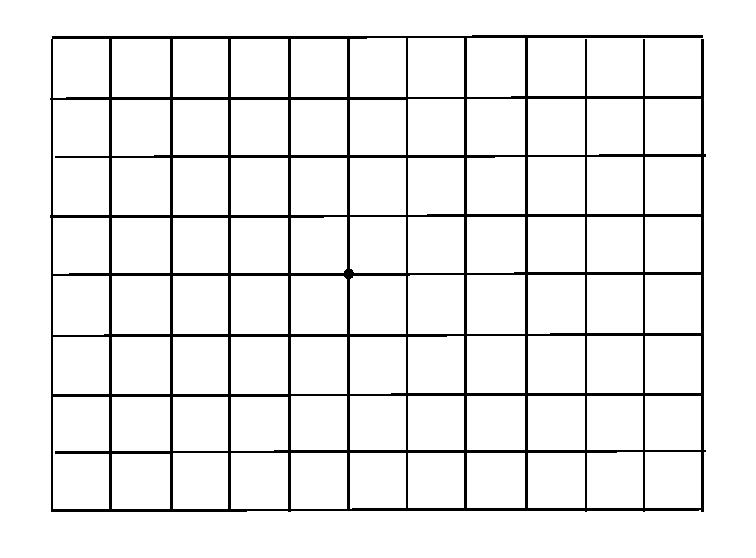
\includegraphics[width=11cm,height=8cm]{basic_grid2.pdf}
\caption{}
\end{figure}
 
To obtain a finite-difference method, we need to approximate the partial derivatives
with respect to $t$ and $x$ at the grid points. By definition,
the partial derivative of the function $u(x,t)$ with respect to
$t$ at point $(x_k,t_j)$ is
\[
\frac{\pr u}{\pr t}(x_k,t_j)=\lim_{\tau\to 0}\frac{u(x_k,t_j+\tau)-u(x_k,t_j)}{\tau}.
\]
It is natural to expect that
\begin{equation}
\frac{\pr u}{\pr t}(x_k,t_j)\approx \frac{u(x_k,t_j+\tau)-u(x_k,t_j)}{\tau}
\label{a10}
\end{equation}
for sufficiently small $\tau$. What is the error of this formula?
To find this, we assume that $u$ is sufficiently smooth (so that its first and second
derivatives with respect to $t$ are continuous in the interval $(0,T)$ for some $T>0$)
and write the first Taylor polynomial for $u(x_k,t_j+\tau)$:
\[
u(x_k,t_j+\tau)=u(x_k,t_j)+\tau \frac{\pr u}{\pr t}(x_k,t_j)+
\frac{\tau^2}{2}\frac{\pr^2 u}{\pr t^2}(x_k,\xi)
\]
where $\xi$ is between $t_j$ and $t_j+\tau$. It follows that the error,
which is called the {\bf truncation error } and denoted by $\tau_{kj}$,
is given by
\[
\tau_{kj}=\frac{\pr u}{\pr t}(x_k,t_j)-\frac{u(x_k,t_j+\tau)-u(x_k,t_j)}{\tau}=
-\frac{\tau}{2}\frac{\pr^2 u}{\pr t^2}(x_k,\xi).
\]
Thus, if $\frac{\pr^2 u}{\pr t^2}(x,t)$ is bounded for all $x$ and $t$, then
\[
\tau_{kj}=O(\tau).
\]
Formula (\ref{a10}) with $\tau>0$ is called the {\bf forward-difference formula}
for the first derivative.
If in (\ref{a10}) we replace $\tau$ by $-\tau$, we obtain the formula
\begin{equation}
\frac{\pr u}{\pr t}(x_k,t_j)\approx \frac{u(x_k,t_j)-u(x_k,t_j-\tau)}{\tau},
\label{a11}
\end{equation}
which is called the {\bf backward-difference formula} (for the first derivative).
 
To derive a finite difference formula for $\pr^2 u(x_k,t_j)/\pr x^2$, we first write the Taylor series expansions
of $u(x_k+h,t_j)$ and $u(x_k-h,t_j)$ at the point $(x_k,t_j)$:
\begin{eqnarray*}
u(x_k+h,t_j)=u(x_k,t_j)&+&h \frac{\pr u}{\pr x}(x_k,t_j)+
\frac{h^2}{2}\frac{\pr^2 u}{\pr x^2}(x_k,t_j)\\
&+&\frac{h^3}{6}\frac{\pr^3 u}{\pr x^3}(x_k,t_{j})+
\frac{h^4}{24}\frac{\pr^4 u}{\pr x^4}(\xi_1,t_{j}), \\
u(x_k-h,t_j)=u(x_k,t_j)&-&h \frac{\pr u}{\pr x}(x_k,t_j)+
\frac{h^2}{2}\frac{\pr^2 u}{\pr x^2}(x_k,t_j)\\
&-&\frac{h^3}{6}\frac{\pr^3 u}{\pr x^3}(x_k,t_{j})+
\frac{h^4}{24}\frac{\pr^4 u}{\pr x^4}(\xi_2,t_{j}) 
\end{eqnarray*}
for some $\xi_{1}$ between $x_{k}$ and $x_{k}+h$
and some $\xi_{2}$ between $x_{k}-h$ and $x_{k}$. 
The sum of these equations gives us the formula
\begin{multline}
u(x_k+h,t_j)+u(x_k-h,t_j)=2u(x_k,t_j)+ h^2\frac{\pr^2 u}{\pr
x^2}(x_k,t_j)\\
+ \frac{h^4}{24}\left(\frac{\pr^4 u}{\pr
x^4}(\xi_1,t_{j}) +\frac{\pr^4 u}{\pr x^4}(\xi_2,t_{j})\right).
\end{multline}
If $\pr^4 u(x,t)/\pr x^4$ is continuous, we can write this in a more compact form. Indeed, the number
\[
\frac{1}{2}\left(\frac{\pr^4 u}{\pr x^4}(\xi_{1}, t_{j})+\frac{\pr^4 u}{\pr x^4}(\xi_{2},t_{j})\right)
\]
is between
the numbers $\frac{\pr^4 u}{\pr x^4}(\xi_{1},t_{j})$ and $\frac{\pr^4 u}{\pr x^4}(\xi_{2},t_{j})$. Therefore,
by the intermediate value theorem, there is a number $\xi$ between $\xi_{1}$ and $\xi_{2}$ such that
$\frac{1}{2}\left(\frac{\pr^4 u}{\pr x^4}(\xi_{1},t_{j})+\frac{\pr^4 u}{\pr x^4}(\xi_{2},t_{j})\right)
=\frac{\pr^4 u}{\pr x^4}(\xi,t_{j})$. Therefore, we obtain
\begin{equation}
\frac{\pr^2 u}{\pr x^2}(x_k,t_j)=\frac{u(x_{k+1},t_j)-2u(x_k,t_j)+u(x_{k-1},t_j)}{h^2}
-\frac{h^2}{12}\frac{\pr^4 u}{\pr x^4}(\xi,t_{j}), \label{a17}
\end{equation}
where $\xi$ is a number between $x_{k}-h$ and $x_{k}+h$.
This is called the {\bf central difference formula} for $u_xx$. When $u_{xxxx}$ is bounded,
then the truncation error in the central difference approximation is $O(h^2)$.
  
 
Now we are ready to obtain the finite-difference equations that approximate
the heat equation (\ref{a1}). First, we introduce numbers $w_{kj}$ for $k=0,1,\dots,N$ and
$j=0,1,2,\dots$ that approximate the exact solution $u(x,t)$ of Eq. (\ref{a1}) at the grid points
$(x_{k}, t_{j})$:
\[
w_{kj}\approx u(x_{k},t_{j}).
\]
Then, we use Eqs. (\ref{a10}) and (\ref{a17}) to approximate
the corresponding derivatives in the heat equation. As a result we obtain the following
difference equations
\begin{equation}
\frac{w_{k,j+1}-w_{kj}}{\tau}-K
\frac{w_{k+1, j}-2w_{kj}+w_{k-1,j}}{h^{2}}=0, \label{b4}
\end{equation}
for each $k=1, 2, \dots, N-1$ and $j=0, 1, \dots, M-1$. Equation ({\ref{b4})
which approximates our PDE at point $(x_{k},t_{j})$ uses approximations to the solution
not only at this point but also
at three neighbouring points $(x_{k+1},t_{j})$, $(x_{k-1},t_{j})$ and $(x_{k},t_{j+1})$.

In approximating the heat equation by the difference equation \eqref{b4} we
introduced a truncation error of from approximating the $t$ derivative of $O(\tau)$
and another truncation error from approximating the $x$ derivative of $O(h^2)$.
Thus it is natural to expect that the truncation error in the difference
equation \eqref{b4} is of order $O(\tau)+O(h^2)$. However we will meet more 
complicated finite-difference methods where the errors do not simply add, so
we need a proper definition of what we mean by the truncation error of a 
finite-difference approximation.

\begin{definition}
Let us represent a PDE as $D\,u=0$, where $D$ is a differential operator,
and the corresponding difference equation as $D_{f.d.}\,w=0$, where
$D_{f.d.}$ is the finite-difference operator that approximates $D$. Then
the {\bf local truncation error} $\tau_{kj}$ of the finite-difference 
approximation at grid point $(x_k,t_j)$ is 
\[\tau_{kj}=(D_{f.d.}\,u)_{kj},\]
i.e., it is equal to the value of the left hand side of the difference
equation evaluated on the exact solution of the differential equation.
\end{definition}
The local truncation error of
the difference equation (\ref{b4}) is given by
\begin{eqnarray*}
\tau_{kj} &=& (D_{f.d.}\,u)_{kj} =
\frac{u_{k,j+1}-u_{kj}}{\tau}-K
\frac{u_{k+1, j}-2u_{kj}-u_{k-1,j}}{h^{2}} \\
&=& \frac{\pr u}{\pr t}(x_{k},t_{j})-
K\frac{\pr^2 u}{\pr x^2}(x_{k},t_{j})+
\frac{\tau}{2}\frac{\pr^{2} u}{\pr t^{2}}(x_{k},
\xi_{1})- K\frac{h^{2}}{12}\frac{\pr^{4} u}{\pr x^{4}}(\xi,t_{j})\\
&=&\frac{\tau}{2}\frac{\pr^{2} u}{\pr t^{2}}(x_{k},
\xi_{1})- K\frac{h^{2}}{12}\frac{\pr^{4} u}{\pr x^{4}}(\xi,t_{j})\\
&=&O(\tau)+O(h^{2})=O(\tau+h^{2}). 
\end{eqnarray*}
Here we used the notation $u_{kj}=u(x_{k}, t_{j})$. 
So in this case the local truncation error is just the sum of the truncation error
from the finite-difference approximation for the time derivative and
the truncation error from the finite-difference approximation for the space
derivative, as we expected.

Equation (\ref{b4}) can be written as
\begin{equation}
w_{k,j+1}=\left(1-2\gamma\right)w_{kj}+
\gamma\left(
w_{k+1, j}+w_{k-1,j}\right), \label{b5}
\end{equation}
for $k=1,\dots,N-1$ and
$j=0,1,\dots, M-1$. In Eq. (\ref{b5}),
$\gamma\equiv K\tau/h^{2}$. Since the initial condition $u(x,0)=u_{0}(x)$
implies that $w_{k,0}=u_{0}(x_{k})$ for each $k=0, 1, \dots, N$, these values can be used in
Eq. (\ref{b5}) to find the value of $w_{k,1}$ for each $k=1, 2, \dots, N-1$. The boundary conditions
$u(0,t)=u(l,t)=0$ imply that $w_{0,1}=w_{N,1}=0$. Now we know $w_{k,1}$ for each $k=0,1,\dots, N$.
Then the same procedure is applied to find $w_{k,2}$, $w_{k,3}$, etc.


 
 
The method described above is called the {{\bf forward-difference method}.
It can also be written in the matrix form
\begin{equation}
{\bf w}^{(j)}=A{\bf w}^{(j-1)} \quad \hbox{for} \quad j=1,2,\dots, \label{b6}
\end{equation}
where
\begin{equation}
A=\left[
\begin{array}{cccccc}
1-2\gamma &\gamma &0      &\dots  &\dots &0 \\
\gamma &1-2\gamma &\gamma &\ddots  &     &\vdots \\
0      &\gamma &1-2\gamma &\gamma &\ddots &\vdots \\
\vdots &\ddots &\ddots &\ddots &\ddots &0 \\
\vdots &       &\ddots &\ddots &\ddots &\gamma \\
0      &\dots  &\dots  &0      &\gamma &1-2\gamma
\end{array}\right], \quad
{\bf w}^{(j)}=\left[
\begin{array}{c}
w_{1,j} \\
w_{2,j} \\
\vdots \\
\vdots \\
\vdots \\
w_{N-1,j}
\end{array}\right].
\label{b7}
\end{equation}
The forward-difference method for the heat equation is an example of an {\bf explicit finite-difference method}.
It is explicit because we do not need to solve any equations, we just use the explicit formula (\ref{b6}).
\begin{figure}[h]
\centering
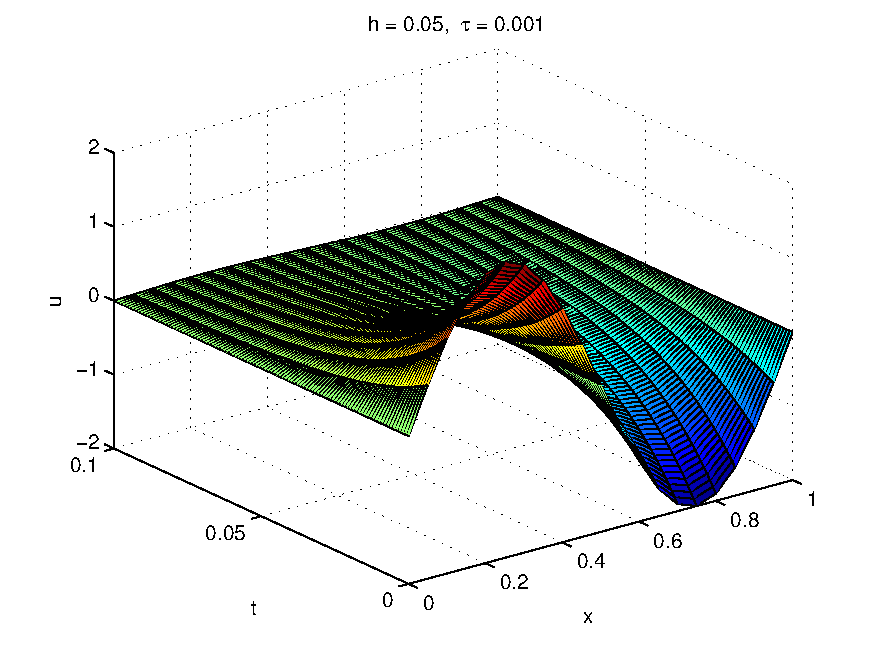
\includegraphics[width=11cm,height=8cm]{forward_diff_fig1.pdf}
\caption{Solution of the forward-difference approximation of the heat equation 
\eqref{a1} with boundary condition \eqref{a2} and initial condition $u(x,0)=2\sin(2\pi x)$ for
$K=1$ and $t\in[0,0.1]$. Step sizes are $h=0.05$ and $\tau=0.001$.}
\label{fig2}
\end{figure}

\begin{figure}[h]
\centering
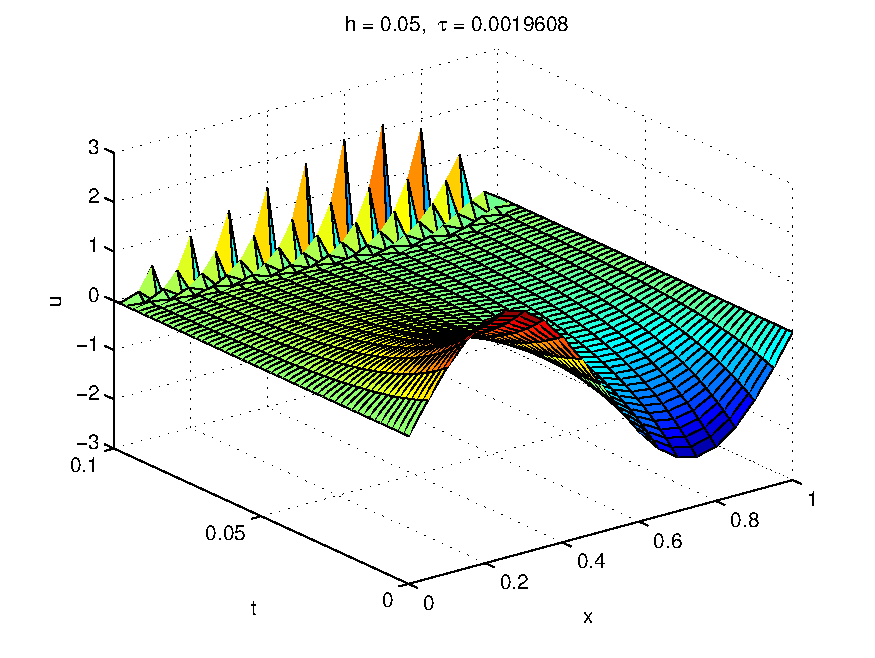
\includegraphics[width=11cm,height=8cm]{forward_diff_fig2.pdf}
\caption{Solution of the forward-difference approximation for the same
equation as in Figure \ref{fig2} but with step sizes are $h=0.05$ and $\tau=0.1/51$.}
\label{fig3}
\end{figure}
A surface plot of the solution $u(x,t)$ of problem (\ref{a1})--(\ref{a3}) for $L=1$, $T=0.1$
and $u_{0}(x)=2 \sin(2\pi x)$, obtained with the help of the forward-difference
method, is shown in Figure \ref{fig2}. So, the method works!

Will it always work? It turns out that it doesn't work if the time step $\tau$ is not small enough.
For example, if we solve the same problem on a grid with a bigger $\tau$, we get what is shown in Figure \ref{fig3}.
So, in this case, the forward-difference method doesn't work properly. The reason for this is that
the finite-difference scheme becomes \textbf{unstable} when $\tau$ is not sufficiently small.


%%%%%%%%%%%%%%%%%%%%%%%%%%%%%%%%%%%%%%%%%%%%%%%%%%%%%%%%%%%%%%%%%%%%%%%%%%%%%%%%

\subsection{Stability}

 
If there are errors $z_{10},
z_{20},\dots, z_{N-1,0}$ in the initial data $w_{10},w_{20},\dots,
w_{N-1,0}$ (or at any particular step, the choice of the initial
step is simply for convenience), the errors propagates to
$w_{11},w_{21},\dots, w_{N-1,1}$, then to 
\linebreak[4]$w_{12},w_{22},\dots,
w_{N-1,2}$, etc. If the errors grow with each time step, then the
difference method in unstable. If they do not grow, it is stable.
How to find out whether a finite-difference method is stable?

Let ${\bf z}^{(0)}=(z_{1}^{(0)}, z_{2}^{(0)},\dots, z_{N-1}^{(0)})^{T}$
be the initial error (or perturbation). Then it follows from (\ref{b6})
that
\[
\tilde{\bf w}^{(1)}=A\tilde{\bf w}^{(0)}=A\left({\bf w}^{(0)}+{\bf z}^{(0)}\right)=A{\bf w}^{(0)}+A{\bf z}^{(0)},
\]
i.e.
\[
{\bf z}^{(1)}=\tilde{\bf w}^{(1)}-{\bf w}^{(1)}=A{\bf z}^{(0)}.
\]
At the $n$-th time step, the error in $\tilde{\bf w}^{(n)}$
due to ${\bf z}^{(0)}$ is ${\bf z}^{(n)}=A^{n}{\bf z}^{(0)}$.
The method is stable if these errors do not grow as $n$ increases, i.e. if and only if
for any initial error ${\bf z}^{(0)}$ we have $\Vert A^{n}{\bf z}^{(0)}\Vert\leq \Vert {\bf z}^{(0)}\Vert$
for all $n$ or, equivalently, $\Vert A{\bf z}^{(0)}\Vert\leq \Vert {\bf z}^{(0)}\Vert$ (here $\Vert\cdot\Vert$
is any vector norm). This, in turn, is
equivalent to the condition that magnitudes of all eigenvalues of $A$ are equal to or smaller than 1,
i.e.
\[
\vert\lambda_{i}\vert\leq 1 \quad \hbox{for} \quad i=1, 2, \dots, N-1.
\]
So, to solve the stability problem we need to calculate the eigenvalues of $A$. 

Calculating the eigenvalues of the matrix in eq.\eqref{b7} analytically is a bit hard.
Instead, we will consider the problem with the boundary conditions
\eqref{a2} replaced by periodic boundary conditions
\begin{equation}
u(x,0)=u(x,L).
\end{equation}
In most cases the stability will not be affected much by this change in boundary
condition. Physically the heat equation with this periodic boundary condition 
would model the heat of a circular rod, where heat flowing out of the right
end flows back in at the left end.

The periodic boundary condition implies that at the boundary point
$k=N$ we have the same value as at $k=0$, but this value is no longer fixed.
Instead we have to use equation \eqref{b5} also for the boundary point $k=N$, 
with the convention that $k=N+1$ is identified with $k=1$. Therefore
eq. \eqref{b7} gets replaced by
\begin{equation}
A=\left[
\begin{array}{cccccc}
1-2\gamma &\gamma &0      &\dots  &0 &\gamma \\
\gamma &1-2\gamma &\gamma &\ddots  &\vdots &0\\
0      &\gamma &1-2\gamma &\gamma &\ddots &\vdots \\
\vdots &\ddots &\ddots &\ddots &\ddots &0 \\
0 &       &\ddots &\ddots &\ddots &\gamma \\
\gamma      &0  &\dots  &0      &\gamma &1-2\gamma
\end{array}\right], \quad
{\bf w}^{(j)}=\left[
\begin{array}{c}
w_{1,j} \\
w_{2,j} \\
\vdots \\
\vdots \\
\vdots \\
w_{N,j}
\end{array}\right].
\label{bp7}
\end{equation}
Luckily this matrix is a
circulant matrix, where each row is equal to the row above, just circularly
shifted to the right by one. 
The eigenvectors of such a matrix are of the form
\[{\bf v} = (1,z,z^2,\dots,z^{N-1})\]
where $z$ is any of the $N$-th roots of unity, $z=\exp(2\pi i n)$ for $n=1,\dots,N$. This knowledge of the
eigenvectors of course makes it simple to calculate the eigenvalues
of the matrix $A$ simply by acting with $A$ on each of the eigenvectors.

Because the matrix for periodic boundary conditions differs from the matrix
for Neumann boundary conditions only in two places, it is plausible that
the eigenvalues will also not differ much between the two cases.

We can also do the stability analysis with periodic boundary conditions
without first writing down
the matrix $A$ but instead directly solving the difference equations. We
refer to this approach as the {\bf Fourier method}.
Let $w_{kj}$ be the exact solution of the difference equation (\ref{b4})
\begin{equation}
\frac{w_{k,j+1}-w_{k,j}}{\tau}-K\frac{w_{k+1,j}-2w_{k,j}+w_{k-1,j}}{h^2}=0 \label{b15}
\end{equation}
(the forward-difference method).
The initial data
\[
z_{k,0}=\tilde{w}_{k,0}-w_{k,0}=\tilde{w}_{k,0}-u_{0}(x_{k}) \quad
\hbox{for} \quad k=0, 1, \dots, N,
\]
propagates with each step in time resulting in another
solution of $\tilde{w}_{kj}$. Let
$z_{kj}=\tilde{w}_{kj}-w_{kj}$ be the error at the mesh point
$(x_{k}, t_{j})$ for each $k=0,1,2, \dots, N$ and $j=0,1, \dots, M$.  $z_{kj}$ satisfies the difference
equation
\begin{equation}
\frac{z_{k,j+1}-z_{k,j}}{\tau}-K\frac{z_{k+1,j}-2z_{k,j}+z_{k-1,j}}{h^2}=0 \label{b16}
\end{equation}
for $k=1,2, \dots, N$ and $j=0,1,\dots,M-1$. (Note that Eq.
(\ref{b16}) coincides with (\ref{b4}). This is because Eq. (\ref{b4}) is linear and homogeneous.) In the Fourier method, we seek a particular solution of
(\ref{b16}) in the form
\begin{equation}
z_{k,j}=\rho_{q}^{j}e^{iqx_{k}}, \quad q\in{\mathbb R}. \label{b17}
\end{equation}
(Here $i=\sqrt{-1}$.) Then the finite-difference method (\ref{b4})
is stable, if all solutions having the form (\ref{b17}) are such that
\[
\vert\rho_{q}\vert\leq 1
\]
for all $q\in{\mathbb R}$.

\vskip 3mm  
Substitution of (\ref{b17}) into (\ref{b16})
yields
\[
\frac{\rho_{q}^{j+1}e^{iqx_{k}}-\rho_{q}^{j}e^{iqx_{k}}}{\tau}-
K\frac{\rho_{q}^{j}\left(e^{iqx_{k+1}}-2e^{iqx_{k}}+e^{iqx_{k-1}}\right)}{h^2}=0
\]
or
\[
\rho_{q}-1 - \gamma \left(e^{iqh}-2+e^{-iqh}\right)=0.
\]
Since
\[
e^{iqh}-2+e^{-iqh}=\left(e^{iqh/2}-e^{-iqh/2}\right)^{2}=-4\sin^{2}
\frac{qh}{2},
\]
we obtain
\[
\rho_{q}=1-4\gamma\sin^{2} \frac{qh}{2}.
\]
The method is stable if
\[
\left\vert 1-4\gamma\sin^{2}\frac{qh}{2}\right\vert\leq 1
\]
for each $q$, which is equivalent to
\[
-1\leq 1-4\gamma\sin^{2}\frac{qh}{2}\leq 1 .
\]
This double inequality is satisfied provided that
\[
0\leq \gamma\sin^{2}\frac{qh}{2}\leq \frac{1}{2}.
\]
Evidently, the last inequality holds for all $q$ if
\begin{equation}
0\leq\gamma \leq \frac{1}{2} \quad \text{ or equivalently} \quad0\leq \tau \leq
\frac{h^2}{2K}. \label{aa}
\end{equation}
Thus, we arrive at the conclusion that the forward-difference method is
stable only if (\ref{aa}) is satisfied.

\vskip 3mm   A method which is stable only if a certain
condition holds is called {\bf conditionally stable}. Thus, the
forward-difference method for the heat equation is conditionally
stable.


%%%%%%%%%%%%%%%%%%%%%%%%%%%%%%%%%
%
% Lecture notes for Numerical Methods for Partial Differential Equations
%
% Chapter 2: Parabolic PDEs
%   Sections 3 and 4
%
%%%%%%%%%%%%%%%%%%%%%%%%%%%%%%%%%

% !TeX root = NumPDE_Lecture_notes.tex

\subsection{Implicit methods}

\subsubsection{Backward-difference method}
 
To obtain a method which is {\bf unconditionally stable}, we consider
an implicit-difference method that results from using the backward-difference formula for
$\pr u/\pr t(x,t)$:
\[
\frac{\pr u}{\pr t}(x_{k},t_{j})=\frac{u(x_{k},t_{j})-u(x_{k},t_{j-1})}{\tau}+
\frac{\tau}{2}\frac{\pr^{2} u}{\pr t^{2}}(x_{k}, \mu_{j}),
\]
where $\mu_{j}\in(t_{j-1},t_{j})$. Using this instead of the forward-difference formula
yields the following difference equation
\begin{equation}
\frac{w_{kj}-w_{k,j-1}}{\tau}-K
\frac{w_{k+1, j}-2w_{kj}+w_{k-1,j}}{h^{2}}=0 \label{x9}
\end{equation}
for $k=1, 2, \dots, N-1$ and $j=1, 2, \dots,M$. This equation is different from Eq. (\ref{b4})
and cannot be solved using a procedure as straightforward as that
in the forward-difference method.

 
 
Equation (\ref{x9}) can be rewritten as
\begin{equation}
(1+2\gamma)w_{kj}-\gamma (w_{k+1, j}+w_{k-1, j})=w_{k,j-1} \label{x10}
\end{equation}
for $k=1, 2, \dots, N-1$ and $j=1, 2, \dots,M$, or, equivalently,
\begin{equation}
A{\bf w}^{(j)}={\bf w}^{(j-1)} \quad \hbox{for} \quad j=1,2,\dots, \label{x11}
\end{equation}
where
\begin{equation}
A=\left[
\begin{array}{cccccc}
1+2\gamma &-\gamma &0      &\dots  &\dots &0 \\
-\gamma &1+2\gamma &-\gamma &\ddots  &     &\vdots \\
0      &-\gamma &1+2\gamma &-\gamma &\ddots &\vdots \\
\vdots &\ddots &\ddots &\ddots &\ddots &0 \\
\vdots &       &\ddots &\ddots &\ddots &-\gamma \\
0      &\dots  &\dots  &0      &-\gamma &1+2\gamma
\end{array}\right], \quad
{\bf w}^{(j)}=\left[
\begin{array}{c}
w_{1,j} \\
w_{2,j} \\
\vdots \\
\vdots \\
\vdots \\
w_{N-1,j}
\end{array}\right].
\label{x12}
\end{equation}
If we know ${\bf w}^{(j-1)}$, Eq. (\ref{x11}) represents a system of linear equations for
${\bf w}^{(j)}$ which can be solved, e.g., by the double-sweep method that we will describe in 
the next subsection.

The finite-difference method described above is called the {\bf backward-difference method}. It is an example
of {\bf implicit} finite-difference methods.

 
 
Now let us investigate the stability of the backward-difference scheme
by the Fourier method.
If we introduce the error $z_{k0}=w_{k0}-u_{0}(x_{k})$ into the initial condition, it
will propagate with each step in time. Let $z_{kj}=w_{kj}-u_{0}(x_{k},t_{j})$ be
the error at the mesh point $(x_{k}, t_{j})$ for each $k=0,1,2, \dots, N$
and $j=0,1, \dots$.
It follows from (\ref{x9}) that $z_{kj}$ satisfies the difference equation
\begin{equation}
\frac{z_{kj}-z_{k,j-1}}{\tau}-K
\frac{z_{k+1, j}-2z_{kj}+z_{k-1,j}}{h^{2}}=0  \label{c15}
\end{equation}
for $k=1, 2, \dots, N-1$ and $j=1, 2, \dots, M$.
We seek a particular solution of
(\ref{c15}) in the form
\begin{equation}
z_{k,j}=\rho_{q}^{j}e^{iqx_{k}}, \quad q\in{\mathbb R}. \label{c16}
\end{equation}
The finite-difference method (\ref{x9}) is stable, if
\[
\vert\rho_{q}\vert\leq 1
\]
for all $q$.

 
 
Substitution of (\ref{c16}) into (\ref{c15}) yields
\[
e^{iqx_{k}}\left(\rho_{q}^{j}-\rho^{j-1}\right)-
\gamma\rho_{q}^{j}\left(e^{iqx_{k+1}}-2e^{iqx_{k}}+e^{iqx_{k-1}}\right)=0
\]
or
\[
1-\frac{1}{\rho_{q}}-
\gamma\left(e^{iqh}-2+e^{-iqh}\right)=0.
\]
Since
\[
e^{iqh}-2+e^{-iqh}=\left(e^{iqh/2}-e^{-iqh/2}\right)^{2}=-4\sin^{2} \frac{qh}{2},
\]
we obtain
\[
\rho_{q}=\frac{1}{1+4\gamma\sin^{2} \frac{qh}{2}}.
\]
Evidently, $\vert\rho_{q}\vert\leq 1$ for all $q$, and therefore, the method is stable.
Note that the method is {\bf unconditionally stable} (independent
of the choice of $\gamma=K\tau/h^{2}$). It can be shown that
its local truncation
error is $O(\tau+h^{2})$ (the same as in the forward-difference method).

\subsubsection{Double-sweep algorithm}
 
\textbf{The double-sweep method.} How to solve system (\ref{x10})? This system is tridiagonal. The most efficient algorithm
of solving such systems is called {\bf the double-sweep method}. Consider the following
tridiagonal system:
\begin{equation}
A_{i}v_{i-1}-C_{i}v_{i}+B_{i}v_{i+1}=F_{i} \quad \hbox{for}\quad i=1, \dots, N-1;
\quad v_{0}=v_{N}=0; \label{y22}
\end{equation}
where the coefficients $A_{i}$, $B_{i}$ and $C_{i}$ satisfy the conditions
\begin{equation}
A_{i}, B_{i}, C_{i} > 0, \quad  C_{i} \geq A_{i} + B_{i}.  \label{y23}
\end{equation}
(One can verify that system (\ref{x10}) satisfies the conditions (\ref{y23}).)
To solve (\ref{y22}), we will seek $\alpha_{i}$ and $\beta_{i}$ such that
\begin{equation}
v_{i-1}=\alpha_{i}v_{i}+\beta_{i}  \quad  \hbox{for} \quad
i=1, 2, \dots, N.  \label{y24}
\end{equation}
Substitution of (\ref{y24}) into (\ref{y22}) yields
\begin{equation}
(\alpha_{i}A_{i}-C_{i})v_{i}+B_{i}v_{i+1}+\beta_{i}A_{i}-F_{i}=0 \quad \hbox{for}\quad i=1, \dots, N-1. \label{y25}
\end{equation}
From (\ref{y24}), we also have
\[
v_{i}=\alpha_{i+1}v_{i+1}+\beta_{i+1}  \quad  \hbox{for} \quad
i=0, 1, \dots, N-1.
\]
Substituting this into (\ref{y25}), we find that
\[
[(\alpha_{i}A_{i}-C_{i})\alpha_{i+1}+B_{i}]v_{i+1}+[
(\alpha_{i}A_{i}-C_{i})\beta_{i+1}+\beta_{i}A_{i}-F_{i}]=0
\]
for $i=1, \dots, N-1$.
This equation is satisfied if the two expressions in the square brackets are both zero. 
This leads to the following recursive formulas:
\begin{equation}
\alpha_{i+1}=\frac{B_{i}}{C_{i}-\alpha_{i}A_{i}}, \quad
\beta_{i+1}=\frac{\beta_{i}A_{i}-F_{i}}{C_{i}-\alpha_{i}A_{i}}, \quad
\hbox{for}\quad i=1, \dots, N-1. \label{y26}
\end{equation}
Now if $\alpha_{1}$ and  $\beta_{1}$ are known, then $\alpha_{i}$ and  $\beta_{i}$ for $i=2, 3, \dots, N$
can be computed from Eqs. (\ref{y26}).  $\alpha_{1}$ and  $\beta_{1}$ can be determined from Eq. (\ref{y24}) and
the fact that $v_{0}=0$. Indeed
\[
v_{0}= \alpha_{1}v_{1}+\beta_{1} \quad \hbox{and} \quad v_{0}=0 \quad \Rightarrow \quad
\alpha_{1}v_{1}+\beta_{1}=0.
\]
To satisfy the last equation, we choose $\alpha_{1}=0$ and $\beta_{1}=0$. Once we know all $\alpha_{i}$
and $\beta_{i}$, we compute $v_{N-1}, v_{N-2}, \dots, v_{1}$ using formula (\ref{y24}).

   
Now let's show that conditions (\ref{y23}) are sufficient for the double-sweep method to work. Numbers $\alpha_{i}$ and $\beta_i$ are well-defined
by Eqs. (\ref{y26}) provided that $C_{i}-\alpha_{i}A_{i}\neq 0$ for $i=1,\dots,N$.
First we show that $0\leq\alpha_i < 1$ for $i=1,\dots,N$. We will show this by induction. Since $\alpha_1=0$, it satisfies
the required inequality. Now we need to show that if $0\leq\alpha_{i}<1$ for some
$i\geq 1$, then $0\leq\alpha_{i+1}<1$. it follows from (\ref{y23}) that
\[
C_{i}-\alpha_{i}A_{i}> A_i + B_i- \alpha_{i}A_{i} > B_i \quad
\Rightarrow \quad \alpha_{i+1}=\frac{B_{i}}{C_{i}-\alpha_{i}A_{i}} < 1.
\]
So, all $\alpha_i$ satisfy $0\leq\alpha_i < 1$. Therefore,
\[
C_{i}-\alpha_{i}A_{i}> A_i + B_i- \alpha_{i}A_{i} > B_i >0 \quad \hbox{for} \ \ i=1,\dots,N,
\]
as required.


\vskip 0.5cm  
\emph{Is it possible to generalise the double-sweep method to the case
when we have non-zero boundary conditions?} The answer is `Yes', and it is not difficult.

Suppose that we need to solve the same equations (\ref{y22}), but with non-zero boundary conditions:
\[
v_{0}=A, \quad v_{N}=B.
\]
The only thing that we need to modify is the choice of $\alpha_{1}$ and $\beta_{1}$. It follows from Eq. (\ref{y24})
and the boundary condition that
\[
\alpha_{1}v_{1}+\beta_{1}=A.
\]
To satisfy this we simply choose
\[
\alpha_{1}=0, \quad \beta_{1}=A.
\]
Boundary  condition $v_{N}=B$ is taken into account automatically when
$v_{N-1}$ is computed using Eq. (\ref{y24}).

\vskip 0.5cm  
The double-sweep method can also be generalised for
the following boundary conditions:}
\[
v_{0}=\lambda v_1+A \quad \hbox{and} \quad v_{N}=\mu v_{N-1} + B,
\]
where $\lambda$, $\mu$, $A$ and $B$ are constants and $\vert\lambda\vert\leq 1$, $\vert\mu\vert\leq 1$. (Prove this!)

%%%%%%%%%%%%%%%%%%%%%%%%%%%%%%%%%%%%%%%%%%%%%%%%%%%%%%%%%%%%%%%%%%%%%%%%%%%%%%%%%%%%%%%%%%%%%%%%%%%%%%%%%%%
\subsubsection{Richardson method}

\emph{How to improve the order of approximation
of the heat equation by finite-difference schemes?} The easiest way
to obtain a finite-difference method whose truncation error is
$O(\tau^{2}+h^{2})$ is to replace the forward (backward)
difference formulas for $u_{t}$ with the central difference
formula:
\begin{equation}
\frac{\pr u}{\pr t}(x_k,t_j)=\frac{u(x_k,t_j+\tau)-u(x_k,t_j-\tau)}{2\tau}-
\frac{\tau^2}{6}\frac{\pr^3 u}{\pr t^3}(x_k,\xi) \label{aa15}
\end{equation}
[It is an exercise for you to derive this formula.]
This leads to the Richardson method, which for the heat equation gives
\begin{equation}
\frac{w_{k,j+1}-w_{k,j-1}}{2\tau}-K \frac{w_{k+1,
j}-2w_{kj}+w_{k-1,j}}{h^{2}}=0. \label{d4}
\end{equation}
(for $k=1, 2, \dots, N-1$ and $j=1, 2, \dots, M-1$). 
\footnote{This was the first published finite-difference methods for PDEs, introduced by Lewis Fry Richardson already in 1911 in
``The Approximate Arithmetical Solution by Finite Differences of Physical Problems Involving Differential Equations, with an Application to the Stresses in a Masonry Dam'', Philosophical Transactions of the Royal Society of London A 210, pp.307 -- 357.}


 
\begin{problem} Show that the Richardson method
has the local truncation error $O(\tau^{2}+h^{2})$.
\end{problem}
\begin{solution}
The local truncation error for Richardson's
method is
\begin{equation}
\tau_{kj}=\frac{u_{k,j+1}-u_{k,j-1}}{2\tau}-K \frac{u_{k+1,
j}-2u_{kj}+u_{k-1,j}}{h^{2}}. \label{d5}
\end{equation}
Here $u_{kj}=u(x_{k},t_{j})$. Expanding $u_{k,j\pm
1}=u(x_{k},t_{j\pm 1})=u(x_{k},t_{j}\pm \tau)$ in Taylor's series at
point $(x_{k},t_{j})$, we obtain
\begin{eqnarray}
&&u_{k,j+1}=u_{kj}+\tau \frac{\pr u}{\pr t}(x_k,t_j)+
\frac{\tau^2}{2}\frac{\pr^2 u}{\pr t^2}(x_k,t_j)+O(\tau^3),   \nonumber \\
&&u_{k,j-1}=u_{kj}-\tau \frac{\pr u}{\pr t}(x_k,t_j)+
\frac{\tau^2}{2}\frac{\pr^2 u}{\pr t^2}(x_k,t_j)+O(\tau^3).
\nonumber
\end{eqnarray}
It follows that
\begin{equation}
\frac{u_{k,j+1}-u_{k,j-1}}{2\tau}=\frac{\pr u}{\pr
t}(x_k,t_j)+O(\tau^2). \label{d6}
\end{equation}
Expanding $u_{k\pm 1,j}=u(x_{k\pm 1},t_j)=u(x_{k}\pm h,t_{j})$ in
Taylor's series at point $(x_{k},t_{j})$, we find that
\begin{eqnarray}
&&u_{k+1,j}=u_{kj}+h \frac{\pr u}{\pr x}(x_k,t_j)+
\frac{h^2}{2}\frac{\pr^2 u}{\pr x^2}(x_k,t_j)+
\frac{h^3}{6}\frac{\pr^3 u}{\pr x^3}(x_k,t_j)+O(h^4),   \nonumber \\
&&u_{k-1,j}=u_{kj}-h \frac{\pr u}{\pr x}(x_k,t_j)+
\frac{h^2}{2}\frac{\pr^2 u}{\pr x^2}(x_k,t_j)-
\frac{h^3}{6}\frac{\pr^3 u}{\pr x^3}(x_k,t_j)+O(h^4).   \nonumber
\end{eqnarray}
Hence,
\begin{equation}
\frac{u_{k+1, j}-2u_{kj}+u_{k-1,j}}{h^{2}}= \frac{\pr^2 u}{\pr
x^2}(x_k,t_j)+O(h^2). \label{d7}
\end{equation}
Substitution of (\ref{d6}) and (\ref{d7}) in Eq. (\ref{d5}) yields
\[
\tau_{kj}=\frac{\pr u}{\pr t}(x_k,t_j)-K \frac{\pr^2 u}{\pr
x^2}(x_k,t_j) +O(\tau^2)+O(h^2).
\]
Taking into account the fact that $u(x,t)$ satisfies the heat equation,
we obtain
\[
\tau_{kj}=O(\tau^2+h^2).
\]
\end{solution}
 
\begin{problem}
Investigate the
stability of Richardson's method, given by (\ref{d4}), by the
Fourier method.
\end{problem}
\begin{solution}
If $w_{kj}$ and $\tilde{w}_{kj}$ are two
solutions of the difference equation (\ref{d4}) that correspond to
different initial conditions, then the perturbation (error)
$z_{kj}=\tilde{w}_{kj}-w_{kj}$ satisfies the homogeneous difference
equation
\begin{equation}
\frac{z_{k,j+1}-z_{k,j-1}}{2\tau}-K \frac{z_{k+1,
j}-2z_{kj}+z_{k-1,j}}{h^{2}}=0. \label{d8}
\end{equation}
We seek a particular solution of (\ref{d8}) in the form
\[
z_{k,j}=\rho_{q}^{j}e^{iqx_{k}}.
\]
Substituting this into (\ref{d8}), we obtain
\[
e^{iqx_{k}}\left(\rho_{q}^{j+1}-\rho_{q}^{j-1}\right)-
2\gamma\rho_{q}^{j}
\left(e^{iqx_{k+1}}-2e^{iqx_{k}}+e^{iqx_{k-1}}\right)=0
\]
or
\[
\rho^{2}_{q}-1- 2\gamma\rho_{q} \left(e^{iqh}-2+e^{-iqh}\right)=0 .
\]
Since
\[
e^{iqh}-2+e^{-iqh}=\left(e^{iqh/2}-e^{-iqh/2}\right)^{2}=-4\sin^{2}
\frac{qh}{2},
\]
we obtain
\[
\rho^{2}_{q}+\left(8\gamma\sin^{2} \frac{qh}{2}\right)\rho_{q}-1=0.
\]
One of the roots of this quadratic equation, namely,
\[
\rho_{q}=-4\gamma\sin^{2} \frac{qh}{2}- \sqrt{16\gamma^2\sin^{4}
\frac{qh}{2}+1},
\]
is greater than $1$ in magnitude for any $q$ such that $\sin(qh/2)\neq 0$. Thus, Richardson's
method is (unconditionally) unstable.
\end{solution}


\subsubsection{Crank-Nicolson method} 

Let $\delta_{x}^{2}$ be a finite-difference operator defined by
\begin{equation}
\delta_{x}^{2}w_{kj}=w_{k+1, j}-2w_{kj}+w_{k-1,j}. \label{cc0}
\end{equation}
Consider the initial boundary value problem for
the heat equation
\begin{eqnarray}
&&\frac{\pr u}{\pr t}(x,t) = K\frac{\pr^{2} u}{\pr x^{2}}(x,t), \quad
0<x< L, \quad 0<0<T,   \label{c1} \\
&&u(0, t) = u(L, t)=0 \quad \hbox{for} \quad t>0,   \label{c2} \\
&&u(x, 0) = u_{0}(x).   \label{c3}
\end{eqnarray}
With the help of the above notation the (explicit) forward-difference method for Eq. (\ref{c1}) can be written as
\begin{equation}
\frac{w_{k,j+1}-w_{kj}}{\tau}-K\frac{\delta_{x}^{2}w_{kj}}{h^2}=0, \label{cc4}
\end{equation}
the (implicit) backward-difference method can be written as
\begin{equation}
\frac{w_{k,j+1}-w_{kj}}{\tau}-K\frac{\delta_{x}^{2}w_{k,j+1}}{h^2}=0. \label{cc5}
\end{equation}
A better method is obtained by averaging the forward-difference
method (\ref{cc4}) and the backward-difference method (\ref{cc5}).
Adding Eq. (\ref{cc4}) to Eq. (\ref{cc5}) with weights $1/2$, we
obtain the difference equation
\begin{equation}
\frac{w_{k,j+1}-w_{k,j}}{\tau}- \frac{K}{2h^{2}}\left(
\delta_{x}^{2}w_{kj}+\delta_{x}^{2}w_{k,j+1}\right)=0 \label{qq14}
\end{equation}
or, equivalently,
\begin{equation}
w_{k,j+1}-w_{k,j}-\frac{\gamma}{2}\left( w_{k+1,
j}-2w_{kj}+w_{k-1,j}+ w_{k+1, j+1}-2w_{k,j+1}+w_{k-1,j+1}\right)=0
\label{qq15a}
\end{equation}
where $\gamma=K\tau/h^2$.
This method is called the {\bf Crank-Nicolson method}. It can be
shown that the local truncation error of the  Crank-Nicolson method
is $O(\tau^{2}+h^{2})$ (see problem sheet).

   
In matrix form, Eq. (\ref{qq15a}) can be
written as
\begin{equation}
A{\bf w}^{(j+1)}=B{\bf w}^{(j)} \quad \hbox{for} \quad
j=0,1,2,\dots, \label{qq15}
\end{equation}
where
\[\begin{split}
A&=\left[
\begin{array}{cccccc}
1+\gamma &-\gamma/2 &0      &\dots  &\dots &0 \\
-\gamma/2 &1+\gamma &-\gamma/2 &\ddots  &     &\vdots \\
0      &-\gamma/2 &1+\gamma &-\gamma/2 &\ddots &\vdots \\
\vdots &\ddots &\ddots &\ddots &\ddots &0 \\
\vdots &       &\ddots &\ddots &\ddots &-\gamma/2 \\
0      &\dots  &\dots  &0      &-\gamma/2 &1+\gamma
\end{array}\right], \\
B&=\left[
\begin{array}{cccccc}
1-\gamma &\gamma/2 &0      &\dots  &\dots &0 \\
\gamma/2 &1-\gamma &\gamma/2 &\ddots  &     &\vdots \\
0      &\gamma/2 &1-\gamma &\gamma/2 &\ddots &\vdots \\
\vdots &\ddots &\ddots &\ddots &\ddots &0 \\
\vdots &       &\ddots &\ddots &\ddots &\gamma/2 \\
0      &\dots  &\dots  &0      &\gamma/2 &1-\gamma
\end{array}\right].
\end{split}\]
If we know ${\bf w}^{(j)}$, we can find ${\bf w}^{(j+1)}$ by solving the tridiagonal linear
system (\ref{qq15}) by the double-sweep method.

\vskip 0.5cm  
To investigate the stability of the Crank-Nicolson method, we employ
the Fourier method. If $z_{kj}=w_{kj}-\tilde{w}_{kj}$, then
\begin{equation}
z_{k,j+1}-z_{k,j}-\frac{\gamma}{2} \left(z_{k+1,
j}-2z_{kj}-z_{k-1,j}+ z_{k+1, j+1}-2z_{k,j+1}+z_{k-1,j+1}\right)=0
\label{qq16}
\end{equation}
for $k=1,2, \dots, N-1$ and $j=1,2, \dots$. We seek a particular
solution of (\ref{qq16}) in the form
\begin{equation}
z_{k,j}=\rho_{q}^{j}e^{iqx_{k}}, \quad q\in{\mathbb R}. \label{qq17}
\end{equation}
Then, the finite-difference method (\ref{qq15a}) is
stable, if
\[
\vert\rho_{q}\vert\leq 1
\]
for all $q$.

   
Substitution of (\ref{qq17}) into (\ref{qq16})
yields
\begin{multline}
0=e^{iqx_{k}}\left(\rho_{q}^{j+1}-\rho_{q}^{j}\right)\\
-\frac{\gamma}{2}\left[\rho_{q}^{j}
\left(e^{iqx_{k+1}}-2e^{iqx_{k}}+e^{iqx_{k-1}}\right)
+\rho_{q}^{j+1}\left(e^{iqx_{k+1}}-2e^{iqx_{k}}+e^{iqx_{k-1}}\right)
\right]
\end{multline}
or
\begin{multline*}
0=\rho_{q}-1- \frac{\gamma}{2} \left[e^{iqh}-2+e^{-iqh}+
\rho_{q}\left(e^{iqh}-2+e^{-iqh}\right) \right]\\
\Rightarrow
\quad 0=\rho_{q}-1-
\frac{\gamma}{2}(\rho_{q}+1)\left(e^{iqh}-2+e^{-iqh}\right).
\end{multline*}
Since
\[
e^{iqh}-2+e^{-iqh}=\left(e^{iqh/2}-e^{-iqh/2}\right)^{2}=-4\sin^{2}
\frac{qh}{2},
\]
we obtain
\[
\rho_{q}-1+(\rho_{q}+1) 2\gamma\sin^{2} \frac{qh}{2}=0 \quad
\Rightarrow \quad \rho_{q}=\frac{1-2\gamma\sin^{2}
\frac{qh}{2}}{1+2\gamma\sin^{2} \frac{qh}{2}}.
\]
To find out whether $\vert\rho_{q}\vert \leq 1$, we consider the function
$f(\alpha)=\frac{1-\alpha}{1+\alpha}$ for $\alpha\in[0,\infty)$. Since
$f'(\alpha)=-\frac{2}{(1+\alpha)^2} < 0$ for all $\alpha\in[0,\infty)$,
it is a decreasing function.
In addition to this, we have $f(0)=1$ and $\lim_{\alpha\to\infty}f(\alpha)=-1$.
We conclude that
$-1< f(\alpha) \leq 1$ for $\alpha\geq 0$. Therefore, $\vert\rho_{q}\vert \leq 1$
for all $q\in\mathbb{R}$, and
the Crank-Nicolson method is unconditionally stable.



%%%%%%%%%%%%%%%%%%%%%%%%%%%%%%%%%%%%%%%%%%%%%%%%%%%%%%%%%%%%%%%%%%%%%%%%%%%%%%%%%%%%



\subsection{Consistency, stability, and convergence}

 
By definition, a finite-difference approximation to a differential equation
is {\bf consistent} with this differential equation if local truncation errors
tend to zero as the step size goes to zero, i.e.
\[
\max_{k,j}\vert \tau_{ki}(h,\tau)\vert \to 0 \ \ {\rm as} \ \ h,\tau \to 0.
\]
Finite difference equation for PDEs arising in initial value
problems may display a phenomenon which has no counterpart in
ordinary differential equations. Successive reduction of step
sizes in $x$ and $t$ may generate a finite difference solution
which is stable, but which may converge to the solution of a
different differential equation. For example, the Du Fort -
Frankel method for solving the heat equation
\begin{equation}
\frac{\partial u}{\partial t}- \frac{\partial^{2}u}{\partial
x^{2}}=0 \label{ww1}
\end{equation}
is given by
\[
\frac{w_{k,j+1}-w_{k,j-1}}{2\tau}- \frac{w_{k+1,
j}-w_{k,j-1}-w_{k,j+1}+w_{k-1,j}}{h^{2}}=0.
\]
It can be shown that this method is always stable and has
the local truncation error
\[
\tau_{kj}=O\left(\tau^2+h^2+\frac{\tau^2}{h^2}\right).
\]
Thus, the Du Fort-Frankel formula is consistent with Eq. (\ref{ww1}) only
if $\tau$ goes to zero faster than $h$. If they go to zero
at the same rate, so that $\tau/h=\beta$ is fixed, then this approximation
is consistent not with the diffusion equation but with the hyperbolic equation
\[
\frac{\partial u}{\partial t}- \frac{\partial^{2}u}{\partial
x^{2}}+ \beta^2\frac{\partial^{2}u}{\partial t^{2}}=0.
\]





    
By definition, a finite-difference method is said to be {\bf convergent}
if the total error of the method
\[
E=\max\limits_{k,j}\vert u_{kj}-w_{kj}\vert
\]
tends to zero as $h\to 0$ and $\tau\to 0$:
\[
E \to 0 \quad {\rm as} \quad h\to 0 \quad {\rm and} \quad \tau\to 0.
\]
We know that an approximation for the initial boundary value problem (\ref{c1})--(\ref{c3})
can be obtained using the forward-difference method
\begin{multline}
w_{k,j+1}=\left(1-2\gamma\right)w_{kj}+
\gamma\left( w_{k+1, j}+w_{k-1,j}\right)\\ {\rm for}
\quad k=1,2,\dots,N-1, 
j=0,1,\dots,M-1, \quad\quad \label{c4}
\end{multline}
\begin{align}
w_{0,j}&=w_{N,j}=0  \quad {\rm for}
\quad j=0,1,\dots,M \quad {\rm and} 
 \label{c5} \\w_{k,0}&=u_{0}(x_{k}) \quad {\rm for}
\quad k=1,2,\dots,N-1.\notag
\end{align}
Here $\gamma\equiv K\tau/h^{2}$.
Also, we know that the local truncation error for the method is
\begin{equation}
\tau_{kj}= \frac{u_{k,j+1}-u_{kj}}{\tau}-\frac{\gamma}{\tau}
\left(u_{k+1,j}-2u_{kj}+u_{k-1,j}\right)=O(\tau+h^{2}), \label{c6}
\end{equation}
so that the method is consistent,
and that the method is stable under the condition
\begin{equation}
\gamma \leq \frac{1}{2}. \label{c7}
\end{equation}

\begin{theorem}
If the stability condition (\ref{c7}) is satisfied,  the forward-difference method 
(\ref{c4}), (\ref{c5}) is convergent.
\end{theorem}

\begin{proof}
It follows from (\ref{c6}) that
\begin{equation}
u_{k,j+1}=(1-2\gamma)u_{kj}+\gamma
\left(u_{k+1,j}+u_{k-1,j}\right)+O(\tau^2+h^{2}\tau).  \label{c8}
\end{equation}
Let
\begin{equation}
z_{kj}=u_{kj}-w_{kj}. \label{c9}
\end{equation}
Then it follows from (\ref{c8}) and (\ref{c4}) that
\begin{equation}
z_{k,j+1}=(1-2\gamma)z_{kj}+\gamma
\left(z_{k+1,j}+z_{k-1,j}\right)+O(\tau^2+h^{2}\tau)  \label{c10}
\end{equation}
for $k=1,2,\dots,N-1$ and $j=0,1,\dots,M-1$.
In view of (\ref{c5}),
\begin{equation}
z_{0,j}=z_{N,j}=0,  \quad j=0,1,\dots,M \quad {\rm and} \quad
z_{k,0}=0, \quad k=1,2,\dots,N-1. \label{c11}
\end{equation}
If the stability condition (\ref{c7}) is satisfied, then
all coefficients on the right side of (\ref{c10}) are positive.

By definition of the big-$O$ notation, Eq. (\ref{c10}) implies that for
sufficiently small $\tau$ and $h$
\[
\left\vert z_{k,j+1}-\left[(1-2\gamma)z_{kj}+\gamma
\left(z_{k+1,j}+z_{k-1,j}\right)\right]\right\vert \leq A_{k,j+1} \, \vert\tau^2+h^{2}\tau\vert
\]
for some positive $A_{k,j+1}$. This and the inequality
\[
\vert a\vert = \vert b +(a-b)\vert\leq \vert b\vert + \vert a-b\vert
\]
(which is valid for any $a$ and $b$)
have the consequence that
\begin{equation}
\vert z_{k,j+1}\vert \leq\vert (1-2\gamma)z_{kj}+\gamma
\left(z_{k+1,j}+z_{k-1,j}\right)\vert +A_{k,j+1} \, \vert\tau^2+h^{2}\tau\vert  \label{c10a}
\end{equation}
for  $k=1,2,\dots,N-1$ and $j=0,1,\dots,M-1$. 
(Set $a=z_{k+1,j}$ and $b=\left[(1-2\gamma)z_{kj}+\gamma
\left(z_{k+1,j}+z_{k-1,j}\right)\right]$.)

\vskip 3mm  
Let ${\bf z}^{(j)}=(z_{1j}, z_{2j}, \dots, z_{N-1,j})^{T}$ and let
\[
\Vert {\bf z}^{(j)}\Vert =\Vert {\bf z}^{(j)}\Vert_{\infty}=
\max\limits_{1\leq k\leq N-1}\vert z_{kj}\vert .
\]
It follows from Eq. (\ref{c10}) that
\begin{eqnarray}
\Vert {\bf z}^{(j+1)} \Vert&=&\max\limits_{k}\vert z_{k,j+1} \vert\nonumber\\
&\leq&
\max\limits_{k}\left\{\left\vert
(1-2\gamma)z_{kj}+\gamma
\left(z_{k+1,j}+z_{k-1,j}\right)\right\vert + A_{j+1} \, \vert\tau^2+h^{2}\tau\vert\right\} \nonumber \\
&\leq&(1 -2\gamma)\max\limits_{k}\vert z_{kj}\vert+
\gamma\max\limits_{k}\vert z_{k+1,j}\vert +
\gamma\max\limits_{k}\vert z_{k-1,j}\vert\nonumber\\
&&\qquad\qquad
+A_{j+1} \, \vert\tau^2+h^{2}\tau\vert \nonumber \\
&\leq&\Vert {\bf z}^{(j)} \Vert+A_{j+1} \, \vert\tau^2+h^{2}\tau\vert. \nonumber
\end{eqnarray}
Here $A_{j+1}=\max\limits_{k}A_{k,j+1}$.
This inequality is valid for all $j=0,1,\dots,M-1$.
It follows that
\begin{eqnarray}
\Vert {\bf z}^{(j)} \Vert&\leq&
\Vert {\bf z}^{(j-1)} \Vert +A_{j} \, \vert\tau^2+h^{2}\tau\vert \nonumber \\
&\leq&\Vert {\bf z}^{(j-2)} \Vert +(A_{j}+A_{j-1}) \, \vert\tau^2+h^{2}\tau\vert \nonumber \\
&&\dots\quad \dots\quad \dots\quad \dots\quad \dots\quad \nonumber \\
&\leq&\Vert {\bf z}^{(0)} \Vert +(A_{j}+\dots +A_{1})\, \vert\tau^2+h^{2}\tau\vert \nonumber \\
&\leq&\Vert {\bf z}^{(0)} \Vert +Aj\tau \, \vert\tau+h^{2}\vert=\Vert {\bf z}^{(0)} \Vert +
A t_{j} \, \vert\tau+h^{2}\vert \nonumber
\end{eqnarray}
where
\[
A=\max_{j}A_{j}=\max_{k,j}A_{kj}.
\]
Since ${\bf z}_{0}=0$, we obtain
\begin{equation}
\Vert {\bf z}^{(j)} \Vert \leq A t_{j} \, \vert\tau+h^{2}\vert \leq A T \vert\tau+h^{2}\vert. \label{c13}
\end{equation}
Since this inequality is valid for all $j=0,1,\dots,M$, we obtain
\[
E= \max\limits_{k,j}\vert z_{kj} \vert=\max\limits_{j}\Vert {\bf z}^{(j)} \Vert\leq A T \vert\tau+h^{2}\vert \quad \Rightarrow \quad E\to 0 \quad {\rm as} \quad \tau,h\to 0.
\]
Thus, we have proved that the forward-difference method is convergent.
\end{proof}
Similar statements can be proved for other finite-difference methods.
 
Lax and Richtmyer\footnote{Lax, P.D., and Richtmyer, R.D. (1956). Survey of the stability of linear finite difference equations. Comm. Pure Appl. Math. 9, 267–293.
} and others studied the relation between consistency, stability,
and convergence of the approximations of linear initial value problems by
finite difference equations. The major result of that study is
\begin{theorem}[Lax equivalence theorem]
Given a well-posed initial boundary value problem and a finite
difference approximation to it that satisfies the consistency condition, then
stability is the necessary and sufficient condition for convergence.
\end{theorem}

%%%%%%%%%%%%%%%%%%%%%%%%%%%%%%%%%
%
% Lecture notes for Numerical Methods for Partial Differential Equations
%
% Chapter 2: Parabolic PDEs
%   Sections 5, 6, and 7
%
%%%%%%%%%%%%%%%%%%%%%%%%%%%%%%%%%

% !TeX root = NumPDE_Lecture_notes.tex

\subsection{Non-homogeneous heat equation with non-homogeneous boundary conditions}

 
So far, we considered the homogeneous heat equation with homogeneous
(zero) boundary conditions. Consider first
the non-homogeneous heat equation with homogeneous
boundary conditions, given by
\begin{eqnarray}
&&\frac{\pr u}{\pr t}(x,t) - K\frac{\pr^{2} u}{\pr x^{2}}(x,t)=f(x,t), \quad
0<x< L, \quad 0<t<T,   \label{d1} \\
&&u(0, t) = u(L, t)=0 \quad \hbox{for} \quad t>0,   \label{d2} \\
&&u(x, 0) = u_{0}(x).   \label{d3}
\end{eqnarray}
The generalisation of the forward-difference and backward-difference methods is straightforward.


\vskip 3mm
 
\underline{Forward-difference method}:
\begin{equation}
\frac{w_{k,j+1}-w_{k,j}}{\tau}-K
\frac{w_{k+1, j}-2w_{kj}+w_{k-1,j}}{h^{2}}=f(x_k,t_j). \label{d10}
\end{equation}
\underline{Backward-difference method}:
\begin{equation}
\frac{w_{k,j}-w_{k,j-1}}{\tau}-K
\frac{w_{k+1, j}-2w_{kj}+w_{k-1,j}}{h^{2}}=f(x_k,t_j). \label{d11}
\end{equation}
The non-homogeneous version of the \underline{Crank-Nicolson method} is given
by
\begin{multline}
\frac{w_{k,j+1}-w_{k,j}}{\tau}-
K \frac{w_{k+1,j}-2w_{kj}+w_{k-1,j}+
w_{k+1,j+1}-2w_{k,j+1}+w_{k-1,j+1}}{2h^{2}}\\
=f(x_k,t_j+\tau/2). \label{d12}
\end{multline}
Note that the right hand side of Eq. (\ref{d12}) can be replaced by
$[f(x_k,t_j)+f(x_k,t_{j+1})]/2$ because
\[
f(x_k,t_j+\tau/2)-\frac{1}{2}[f(x_k,t_j)+f(x_k,t_{j+1})]=O(\tau^2).
\]

  
 
Do the above modifications affect the stability of the methods? The answer is NO, because
in spite of the fact that the difference equations are non-homogeneous, the corresponding equations for perturbation
$z_{kj}$ remain the same homogeneous equations as before.




  
 
\textbf{Non-homogeneous boundary conditions}. Consider
the initial boundary value problem
\begin{eqnarray}
&&\frac{\pr u}{\pr t}(x,t) - K\frac{\pr^{2} u}{\pr x^{2}}(x,t)=f(x,t), \quad
0<x< L, \quad 0<t<T,   \label{d13} \\
&&u(0,t)=\mu_{1}(t), \quad u(L,t)=\mu_{2}(t) \quad \hbox{for} \quad t>0, \label{d14} \\
&&u(x, 0) = u_{0}(x),   \label{d15}
\end{eqnarray}
where $\mu_{1}(t)$ and $\mu_{2}(t)$ are some given functions.
The non-homogeneous boundary conditions (\ref{d14}) can be
dealt with in two ways. First, one can simply change
the boundary conditions for $w_{kj}$ by letting
\begin{equation}
w_{0,j}=\mu_{1}(t_j), \quad w_{N,j}=\mu_{2}(t_j). \label{d16}
\end{equation}
Note that for implicit schemes where we employ the double-sweep method, the latter should be modified
in order to allow non-zero boundary conditions.

\vskip 3mm
 
Second, one can reduce problem (\ref{d13})--(\ref{d15}) to an initial boundary
problem with homogeneous boundary conditions. To do this, we choose any function
$g(x,t)$ satisfying the boundary conditions
\begin{equation}
g(0,t)=\mu_{1}(t), \quad g(L,t)=\mu_{2}(t). \label{d17}
\end{equation}
Now if $u(x,t)=v(x,t)+g(x,t)$ and $u(x,t)$ is the solution of
(\ref{d13})--(\ref{d15}), then $v(x,t)$ must satisfy the initial boundary value
problem
\begin{eqnarray}
&&\frac{\pr v}{\pr t}(x,t) - K\frac{\pr^{2} v}{\pr x^{2}}(x,t)=\tilde{f}(x,t), \quad
0<x< L, \quad 0<t<T,   \label{d18} \\
&&v(0,t)=0, \quad v(L,t)=0 \quad \hbox{for} \quad t>0, \label{d19} \\
&&v(x, 0) = v_{0}(x),   \label{d20}
\end{eqnarray}
where
\[
\tilde{f}(x,t)=f(x,t)-
\frac{\pr g}{\pr t}(x,t) + K\frac{\pr^{2} g}{\pr x^{2}}(x,t), \quad
v_{0}(x)=u_{0}(x)-g(x,0).
\]
For example, we can choose the function
\[
g(x,t)=\mu_{1}(t)+[\mu_{2}(t)-\mu_{1}(t)]\frac{x}{L}.
\]



%%%%%%%%%%%%%%%%%%%%%%%%%%%%%%%%%%%%%%%%%%%%%%%%%%%%%%%%%%%%%%%%%%%%%%%%%%%%%%%%%%%%%%%%%%%%%
%%%%%%%%%%%%%%%%%%%%%%%%%%%%%%%%%%%%%%%%%%%%%%%%%%%%%%%%%%%%%%%%%%%%%%%%%%%%%%%%%%%%%%%%%%%%%
%%%%%%%%%%%%%%%%%%%%%%%%%%%%%%%%%%%%%%%%%%%%%%%%%%%%%%%%%%%%%%%%%%%%%%%%%%%%%%%%%%%%%%%%%%%%%

\subsection{Boundary conditions of other types}.

 
In all the problems we discussed so far, the
boundary conditions did not require approximations of any kind.
A different situation arises when we have the boundary conditions for the derivative
of $u$:
\begin{equation}
\frac{\pr u}{\pr x}(0,t)=\mu_{1}(t), \quad
\frac{\pr u}{\pr x}(L,t)=\mu_{2}(t). \label{d21}
\end{equation}
These are known as Dirichlet boundary conditions.
Evidently, we need to approximate these conditions.

\vskip 3mm
 
Consider the non-homogeneous heat equation
\begin{equation}
\frac{\pr u}{\pr t} - K\frac{\pr^{2} u}{\pr x^{2}}=f(x,t), \quad
0<x< L, \quad 0<0<T,   \label{dd1}
\end{equation}
subject to the boundary conditions (\ref{d21}) and the initial condition
\begin{equation}
u(x, 0) = u_{0}(x).   \label{dd2}
\end{equation}
As in the case of non-homogeneous boundary conditions for $u$, the problem
(\ref{d21})--(\ref{dd2}) with non-homogeneous boundary conditions for $u_{x}$
can be reduced to
a problem with homogeneous boundary condition. To do this, we write
$u(x,t)=v(x,t)+g(x,t)$ with any fixed function $g(x,t)$ satisfying conditions
(\ref{d21}). Then for $v(x,t)$, we obtain the problem
\begin{eqnarray}
&&\frac{\pr v}{\pr t} - K\frac{\pr^{2} v}{\pr x^{2}}=\tilde{f}(x,t), \quad
0<x< L, \quad 0<0<T,   \nonumber \\
&&\frac{\pr v}{\pr x}(0,t)=0, \quad
\frac{\pr v}{\pr x}(L,t)=0, \quad
v(x, 0) = v_{0}(x), \nonumber
\end{eqnarray}
where $\tilde{f}(x,t)=f(x,t)-g_{t}(x,t)+Kg_{xx}(x,t)$ and $v_{0}(x)=u_{0}(x)-g(x,0)$.
[An example of function $g$: $g(x,t)=\mu_{1}(t)x+[\mu_{2}(t)-\mu_{1}(t)]x^2/(2L)$.]
Therefore, we will discuss here only the homogeneous conditions
\begin{equation}
\frac{\pr u}{\pr x}(0,t)=0, \quad
\frac{\pr u}{\pr x}(L,t)=0. \label{d22}
\end{equation}
In what follows we restrict our analysis to the boundary condition at $x=0$
(the other boundary condition can be treated similarly).
If we use the two-point forward-difference formula for the derivative
at $(x=0, t=t_{j})$, then
\[
\frac{w_{1,j}-w_{0,j}}{h}=0 .
\]
However, this formula for $u_{x}(0,t)$ has the truncation error $O(h)$,
while in all the methods that we have considered the truncation error
of the relevant difference equations was
at least $O(h^2)$. So, the use of this formula would increase the local
truncation error of these methods.

  
 
Suppose that we use the forward-difference method
to approximate the heat equation (\ref{dd1}) at the interior grid points.
How to approximate the boundary conditions (\ref{d22})
with truncation error $O(h^2)$ for this method?
We will consider two ways of doing this.
In the first one, we add a `false' boundary at
$x=x_{-1}=x_{0}-h$ and assume that the forward-difference scheme
approximates the heat equation at points $(x_{0},t_{j})$ ($j=1,2,\dots$). Then,
we have
\begin{equation}
\frac{w_{0,j+1}-w_{0,j}}{\tau}-K
\frac{w_{1, j}-2w_{0j}+w_{-1,j}}{h^{2}}=f(0,t_j). \label{d23}
\end{equation}
Approximating $u_{x}({0},t_{j})$ by the central difference formula
(whose truncation error is $O(h^2)$), we find that
\begin{equation}
\frac{w_{1,j}-w_{-1,j}}{2h}=0. \label{d24}
\end{equation}
Eliminating $w_{-1,j}$ from Eqs. (\ref{d23}) and (\ref{d24}), we obtain
\begin{equation}
w_{0,j+1}=(1-2\gamma)w_{0,j}+2\gamma w_{1,j}+\tau f(0,t_j). \label{d25}
\end{equation}
This is an explicit formula that relates the boundary values at the time levels
$t_{j}$ and $t_{j+1}$.

  
 
Similarly, for the boundary condition at $x=L$, one can obtain the formula
\begin{equation}
w_{N,j+1}=(1-2\gamma)w_{N,j}+2\gamma w_{N-1,j}+\tau f(L,t_j). \label{d26}
\end{equation}

  
 
In another (more general) technique which leads to Eqs. (\ref{d25}) and
(\ref{d26}), we expand $u(x_{1},t_{j})$ in Taylor's series at point
$(x_{0},t_{j})$:
\[
u(x_{1},t_{j})=u(x_{0},t_{j})+h u_{x}(x_0,t_j)+
\frac{h^2}{2}u_{xx}(x_0,t_j)+O(h^3).
\]
Taking account of the boundary condition and the fact that $u(x,t)$ is
the solution of the heat equation, we find that
\begin{eqnarray}
u(x_{1},t_{j})=u(x_{0},t_{j})&+&
\frac{h^2}{2K}\left(\frac{\pr u}{\pr t}(x_0,t_j)-
f(x_0,t_j)\right)+O(h^3) \nonumber \\
= u(x_{0},t_{j})&+&
\frac{h^2}{2K}\left(\frac{u(x_0,t_{j+1})-u(x_0,t_{j})}{\tau}-
f(x_0,t_j)\right)\nonumber\\
&+&O(\tau h^2)+O(h^3). \nonumber
\end{eqnarray}
The last equation leads to the difference equation (\ref{d25}).
 
What about the stability of this method?
Evidently, the Fourier method would produce the same answer as before,
because boundary conditions are ignored. The stability can be investigated with the help
of the matrix stability analysis\footnote{See W. F. Ames, Numerical methods for partial differential equation,
Academic Press, 1977.}. The forward-difference method described above can be written in the matrix form
\begin{equation}
{\bf w}^{(j)}=A{\bf w}^{(j-1)}+\tau {\bf F}^{(j-1)} \quad \hbox{for} \quad j=1,2,\dots, \label{d106}
\end{equation}
where
\begin{gather}
A=\left[
\begin{array}{ccccccc}
1-2\gamma &2\gamma &0      &\dots  &\dots  &\dots &0 \\
\gamma &1-2\gamma &\gamma &\ddots  &       &     &\vdots \\
0      &\gamma &1-2\gamma &\gamma &\ddots &      &\vdots \\
\vdots &\ddots &\ddots &\ddots &\ddots &\ddots &\vdots  \\
\vdots &       &\ddots &\ddots &\ddots &\gamma &0 \\
\vdots &       &       &\ddots &\gamma &1-2\gamma &\gamma \\
0      &\dots  &\dots  &\dots  &0      &2\gamma &1-2\gamma
\end{array}\right], \\
{\bf w}^{(j)}=\left[
\begin{array}{c}
w_{0,j} \\
w_{1,j} \\
w_{2,j} \\
\vdots \\
\vdots \\
\vdots \\
w_{N-1,j} \\
w_{N,j}
\end{array}\right], \qquad
{\bf F}^{(j)}=\left[
\begin{array}{c}
f_{0,j} \\
f_{1,j} \\
f_{2,j} \\
\vdots \\
\vdots \\
\vdots \\
f_{N-1,j} \\
f_{N,j}
\end{array}\right].
\label{d107}
\end{gather}
The method will be stable if for all eigenvalues $\lambda$ of $A$,
\[
\vert \lambda\vert\leq 1,
\]
and it can be shown (see W. F. Ames, Numerical methods for partial differential equations)
that this results in the same stability condition $\gamma\leq 1/2$.


  
 
The implicit backward-difference method  for problem
(\ref{d21})--(\ref{dd2}) can be written in the matrix form as follows
\begin{equation}
B{\bf w}^{(j)}={\bf w}^{(j-1)}+\tau {\bf F}^{(j)} \quad \hbox{for} \quad j=1,2,\dots,
\end{equation}
where
\begin{gather}
B=\left[
\begin{array}{ccccccc}
1+2\gamma &-2\gamma &0      &\dots  &\dots  &\dots &0 \\
-\gamma &1+2\gamma &-\gamma &\ddots  &       &     &\vdots \\
0      &-\gamma &1+2\gamma &-\gamma &\ddots &      &\vdots \\
\vdots &\ddots &\ddots &\ddots &\ddots &\ddots &\vdots  \\
\vdots &       &\ddots &\ddots &\ddots &-\gamma &0 \\
\vdots &       &       &\ddots &-\gamma &1+2\gamma &-\gamma \\
0      &\dots  &\dots  &\dots  &0      &-2\gamma &1+2\gamma
\end{array}\right], \\
{\bf w}^{(j)}=\left[
\begin{array}{c}
w_{0,j} \\
w_{1,j} \\
w_{2,j} \\
\vdots \\
\vdots \\
\vdots \\
w_{N-1,j} \\
w_{N,j}
\end{array}\right], \quad
{\bf F}^{(j)}=\left[
\begin{array}{c}
f_{0,j} \\
f_{1,j} \\
f_{2,j} \\
\vdots \\
\vdots \\
\vdots \\
f_{N-1,j} \\
f_{N,j}
\end{array}\right].
\end{gather}
It can be shown that it remains unconditionally stable.
 
More general boundary conditions (Robin boundary conditions)
\begin{equation}
\frac{\pr u}{\pr x}(0,t)+c_{1}(t)u(0,t)=\mu_{1}(t), \quad
\frac{\pr u}{\pr x}(L,t)+c_{2}(t)u(L,t)=\mu_{2}(t), \label{d27}
\end{equation}
where $c_{1}(t)$ and $c_{2}(t)$ are some given functions, can be treated
similarly.


%%%%%%%%%%%%%%%%%%%%%%%%%%%%%%%%%%%%%%%%%%%%%%%%%%%%%%%%%%%%%%%%%%%%%%%%%%%%%%%%%%%%%%%
\subsection{Variable coefficients}.

Consider the parabolic equation
\begin{equation}
\frac{\pr u}{\pr t} =a(x,t)\frac{\pr^{2} u}{\pr x^{2}}+
b(x,t)\frac{\pr u}{\pr x}+c(x,t)u+d(x,t),  \quad 0<x< L, \quad 0<t<T, \label{e1}
\end{equation}
subject to the initial and boundary conditions
\begin{eqnarray}
&&u(x, 0) = u_{0}(x), \label{e2} \\
&&u(0,t)=0, \quad u(L,t)=0.   \label{e3}
\end{eqnarray}
Here we assume that
\begin{equation}
a(x,t)> 0 \quad {\rm for} \quad 0\leq x\leq L, \ \ 0<t<T. \label{e4}
\end{equation}
Most of the previously discussed methods can be generalized to the case of
the initial boundary value problem (\ref{e1})--(\ref{e3}).  How to do this?
 
Employing the two-point forward difference formula for $u_t$ and
the central difference formulae for $u_x$ and $u_{xx}$, we obtain
the following finite-difference approximation for Eq. (\ref{e1}):
\begin{equation}
\frac{w_{k,j+1}-w_{k,j}}{\tau} =a_{kj}\frac{w_{k+1,j}-2w_{k,j}+w_{k-1,j}}{h^{2}}+
b_{kj}\frac{w_{k+1,j}-w_{k-1,j}}{2h}+c_{kj}w_{k,j}+d_{kj},   \label{e5}
\end{equation}
for $k=1, \dots,N-1$ and $j=0, 1,\dots,M-1$. In Eq. (\ref{e5}),
$a_{kj}=a(x_{k},t_{j})$, $b_{kj}=b(x_{k},t_{j})$, etc. Since
the forward difference formula
for $u_tt$ has the truncation error $O(\tau)$, and
the errors of the central difference formulae for $u_x$ and $u_{xx}$
are $O(h^2)$, the local truncation error of the difference equation (\ref{e5}) is
\[
\tau_{kj}=O(\tau+h^2).
\]
This, together with obvious boundary conditions, gives us the explicit method
for solving (\ref{e1})--(\ref{e3}) which is similar to the explicit
forward-difference method for the heat equation that we discussed earlier.
Similarly, if we use the backward difference formula for $u_t$, we obtain
the difference equation
\begin{equation}
\frac{w_{k,j}-w_{k,j-1}}{\tau} =a_{kj}\frac{w_{k+1,j}-2w_{k,j}+w_{k-1,j}}{h^{2}}+
b_{kj}\frac{w_{k+1,j}-w_{k-1,j}}{2h}+c_{kj}w_{k,j}+d_{kj},   \label{e6}
\end{equation}
whose local truncation error is $O(\tau+h^2)$ and which is similar to the implicit
backward-difference method for the heat equation.
 
It can be shown that Crank-Nicolson's technique applied to (\ref{e1}) yields:
\begin{eqnarray}
\frac{w_{k,j+1}-w_{k,j}}{\tau} &=& \frac{a_{k,j+1/2}}{2h^{2}} \,
\delta_{x}^2 \, \left(w_{k,j}+w_{k,j+1}\right)
+\frac{b_{k,j+1/2}}{4h} \, \delta_{x} \,  \left(w_{k,j}+w_{k,j+1}\right)\nonumber \\
&&+\frac{c_{k,j+1/2}}{2} \, \left(w_{k,j}+w_{k,j+1}\right)+d_{k,j+1/2}, \nonumber
\end{eqnarray}
where
\[
a_{k,j+1/2}=\frac{a(x_{k},t_{j})+a(x_{k},t_{j+1})}{2}, \quad
b_{k,j+1/2}=\frac{b(x_{k},t_{j})+b(x_{k},t_{j+1})}{2}, \ \ {\rm etc.}
\]
 
What about the stability of these methods?
If the coefficients $a$, $b$, $c$ and $d$ do not
involve $t$, the stability can be investigated
\footnote{See W. F. Ames, Numerical methods for partial differential equation,
Academic Press, 1977.}. In particular, it can be shown that the explicit method
(\ref{e5}) is stable provided that
\[
\frac{\tau}{h^2}<\frac{1}{2a(x,t)} \quad {\rm for} \quad 0\leq x\leq L, \ \ t>0.
\]

\begin{example}
Consider the two-dimensional heat equation
\begin{equation}
\frac{\partial u}{\partial t}= \frac{\partial^{2}u}{\partial
x^{2}}+ \frac{\partial^{2}u}{\partial y^{2}} \quad \textrm{for} \ \ 0<t<T \label{e7}
\end{equation}
in the circular domain ${\cal D}$:
\[
{\cal D}=\{(x,y) \vert \sqrt{x^2+y^2}< R \},
\]
subject to the boundary condition
\begin{equation}
u(x,y,t)=\mu(x,y,t) \quad \hbox{for} \quad \sqrt{x^2+y^2}= R,  \label{e8}
\end{equation}
and the initial condition
\begin{equation}
u(x,y,0)=u_{0}(x,y) \quad \hbox{for} \quad (x,y)\in{\cal D}.  \label{e9}
\end{equation}
In polar coordinates $(r, \theta)$ [such that $x=r\cos\theta$, $y=r\sin\theta$],
the above initial boundary value problem takes the form
\begin{eqnarray}
&&\frac{\partial u}{\partial t}=\frac{\partial^{2}u}{\partial r^{2}}
+ \frac{1}{r}\frac{\partial u}{\partial r}+
\frac{1}{r^2}\frac{\partial^{2}u}{\partial \theta^{2}}
\quad {\rm in} \quad {\cal D},  \nonumber \\
&&u(r,\theta,t)\vert_{r=R}=\mu(\theta,t), \quad
u(r,\theta, 0)=u_{0}(r,\theta).  \label{e10}
\end{eqnarray}
If the initial and boundary conditions do not involve
$\theta$, i.e. $u_{0}=u_{0}(r)$ and $\mu=\mu(t)$, then
the solutions of problem (\ref{e10}) are rotationally symmetric, i.e.
independent of $\theta$, for all $t>0$. In this case, $(\ref{e10})$
simplifies to
\begin{eqnarray}
&&\frac{\partial u}{\partial t}=\frac{\partial^{2}u}{\partial r^{2}}
+ \frac{1}{r}\frac{\partial u}{\partial r}
\quad {\rm for} \quad 0 < r < R,  \nonumber \\
&&u(r,t)\vert_{r=R}=\mu(t), \quad
u(r, 0)=u_{0}(r).  \label{e11}
\end{eqnarray}
There are two apparent difficulties with problem (\ref{e11}): (i) we have only one boundary condition
and (ii) the term $(1/r)(\pr u/\pr r)$ is singular at $r = 0$.
The first difficulty can be eliminated by using the following condition
\begin{equation}
u_r(0,t)=0.  \label{e12}
\end{equation}
This condition holds for any sufficiently smooth solution of (\ref{e11}). To show this, we assume that $u$ is twice continuously differentiable with respect to both $t$
and $r$ in $D$ and integrate Eq. (\ref{e11}) in $r$ from $0$ to $\eps>0$ with weight $r$:
\[
\int\limits_{0}^{\eps}u_{t}(r,t) r \, dr = \int\limits_{0}^{\eps}\frac{1}{r}\, \frac{\pr}{\pr r}\Bigl(r \, u_{r}(r,t)\Bigr) r \, dr
=r \, u_{r}(r,t)\Bigm\vert_{0}^{\eps}= \eps \, u_{r}(\eps,t).
\]
Hence,
\begin{equation}
u_{r}(\eps,t)=\frac{1}{\eps} \, \int\limits_{0}^{\eps}u_{t}(r,t) r \, dr .  \label{e12b}
\end{equation}
For small $\eps$,
\[\begin{split}
\int\limits_{0}^{\eps}u_{t}(r,t) r \, dr &= \int\limits_{0}^{\eps}(u_{t}(0,t)+O(r)) r \, dr=
u_{t}(0,t)\int\limits_{0}^{\eps} (r + O(r^2)) \, dr \\
&=u_{t}(0,t) \, \frac{\eps^2}{2} + O(\eps^3)
\end{split}\]
Passing to the limit as $\eps\to 0$ in (\ref{e12b}) leads to condition (\ref{e12}):
\[
u_{r}(0,t)=\lim_{\eps\to 0} u_{r}(\eps,t)=\lim_{\eps\to 0} \frac{1}{\eps} \, \int\limits_{0}^{\eps}u_{t}(r,t) r \, dr
=\lim_{\eps\to 0} \frac{1}{\eps} \, \left(u_{t}(0,t) \, \frac{\eps^2}{2} + O(\eps^3) \right)=0.
\]
If we try to approximate the boundary condition (\ref{e12}) by introducing a false boundary at $r=r_{-1}=-h$ in the same way as before,
we will need to use a finite-difference scheme at points $(r_{0},t_j)=(r_{0},t_j)$ and therefore to approximate the term $r^{-1}u_{r}$ at $r=0$.
However, we do not know $\lim_{r\to 0}r^{-1}u_{r}$ and, therefore, cannot approximate it. Nevertheless we can avoid the singularity at $r=0$, if we choose
the grid points in such a way that $r_{0}=h/2$ and $r_{k}=r_0+k h$ for $k=1,\dots,N$ with $h=2L/(2N+1)$. Then we introduce the false boundary at $r_{-1}=-h/2$ and approximate
(\ref{e12}) by the central difference formula
\begin{equation}
\frac{w_{0,j}-w_{-1,j}}{h}=0  \label{e12a}
\end{equation}
whose truncation error is $O(h^2)$.

When the Crank-Nicolson concept is applied to Eq. (\ref{e11}),
we obtain the difference equation for the interior grid points $(r_k,t_j)$:
\begin{equation}
\frac{w_{k,j+1}-w_{k,j}}{\tau}-
\frac{1}{2h^2}\left(\delta_{r}^2+\frac{h}{2r_{k}}\delta_{r}\right)
\left(w_{k,j+1}+w_{kj}\right)=0  \label{e13}
\end{equation}
for $k=1,\dots,N-1)$ and $j=0,\dots,M-1$.
Here $\delta^2_{r}$ and $\delta_{r}$ are finite-difference operators, defined
by
\begin{equation}
\delta^2_{r}w_{kj}=w_{k+1,j}-2w_{kj}+w_{k-1,j} \quad {\rm and} \quad
\delta_{r}w_{kj}=w_{k+1,j}-w_{k-1,j}.  \label{e14}
\end{equation}
For grid points $(r_0,t_j)$, we use the same difference equations with $w_{-1,j}$ eliminated using
(\ref{e12a}), i.e.
\begin{equation}
\frac{w_{0,j+1}-w_{0,j}}{\tau}-
\frac{1}{2h^2}\left(1+\frac{h}{2r_{0}}\right)
\left(w_{1,j+1}-w_{0,j+1}+w_{1,j}-w_{0,j}\right)=0 
\end{equation}
for $j=0, 1, \dots, M-1$.

The local truncation error of the approximation (\ref{e13}) can be shown to be
$O(\tau^2+h^2)$.
\end{example}
 
\begin{example} One of the most well-known equation in mathematical finance is the
the Black-Scholes equation:
\begin{equation}
    \frac{\partial V}{\partial t}+\frac{1}{2}\sigma^{2}S^{2}\frac{\partial^{2} V}{\partial S^{2}}+rS\frac{\partial V}{\partial S}
    -rV=0. \label{BS1}
\end{equation}
Here $V$ is the value of the option, $\sigma$ and $r$ are constants.
$V$ depends on the current value $S$ of the underlying asset and on time $t$.

When this equation describes European call option, it is solved subject
to the following conditions:
\begin{eqnarray}
    &&V(0,t)=0 \ \ \text{for} \ \ t<T, \label{BS2} \\
    &&V(S,t)\rightarrow S-Ee^{-r(T-t)}\text{ as }S\rightarrow\infty\, , \label{BS3} \\
    &&V(S,T)=\max\{S-E,0\}. \label{BS4}
\end{eqnarray}
In Eq. (\ref{BS4}), $E$ is a given positive constant. The problem is to solve
Eq. (\ref{BS1}) backwards in time, i.e. for $t<T$. In principle, Eq. (\ref{BS1})
can be transformed to the heat equation on the whole lines and then solved exactly.
Our task is to obtain a numerical solution.

It is convenient to introduce a new independent variable $\tilde{t}=T-t$
and a new dependent variable $\tilde{V}(S,\tilde{t})=V(S,t)-S+Ee^{-r(T-t)}(1-e^{-S})$. Then problem (\ref{BS1})--(\ref{BS4})
takes the form
\begin{eqnarray}
    &&\frac{\partial \tilde{V}}{\partial \tilde{t}}=\frac{1}{2}\sigma^{2}S^{2}
    \frac{\partial^{2} \tilde{V}}{\partial S^{2}}+rS\frac{\partial \tilde{V}}{\partial S}
    -r\tilde{V}+ f(S, \tilde{t}), \label{BS5} \\
    &&\tilde{V}(0,\tilde{t})=0 \ \ \text{for} \ \ t<T, \label{BS6} \\
    &&\tilde{V}(S,\tilde{t})\rightarrow 0\text{ as }S\rightarrow\infty\, , \label{BS7} \\
    &&\tilde{V}(S,0)=\max\{0,E-S\}-E e^{-S}. \label{BS8}
\end{eqnarray}
Here $f(S, \tilde{t})=E \left(\frac{1}{2}\sigma^2 S^2 - r S\right)\, e^{-r\tilde{t}-S}$.
Problem (\ref{BS5})--(\ref{BS8}) is an initial boundary value problem for a parabolic
equation with variable coefficients.

To solve the problem, we choose sufficiently large $S_{0}$ and define the grid points:
\[
(S_k,\tilde{t}_j)=(hk, \tau j) \ \ \text{for} \ \ k=0,\dots,N \ \ \text{and} \ \ j=0, 1, \dots, M
\]
where $h=S_{0}/N$ and $\tau=T/M$ is the step length in time $\tilde{t}$.

To make sure  that out scheme is stable, we employ the backward-difference formula
for $\partial \tilde{V}/\partial \tilde{t}$ and central difference formulae for
$\partial^{2} \tilde{V}/\partial S^{2}$ and $\partial \tilde{V}/\partial S$.
As  a result, we have
\begin{eqnarray}
    &&\frac{w_{k,j}-w_{k,j-1}}{\tau}=\frac{1}{2}\sigma^{2}S_k^{2}
    \frac{w_{k+1,j}-2w_{k,j}+w_{k-1,j}}{h^2}\nonumber\\
    &&\qquad\qquad\qquad\qquad+rS_k\frac{w_{k+1,j}-w_{k-1,j}}{2h}
    -r w_{k,j}+f_{k,j}, \label{BS9} \\
    &&w_{0,j}=0, \quad w_{N,j}=0 , \label{BS11} \\
    &&w_{k,0}=\max\{0,E-S_k\}-E e^{-S_k}. \label{BS12}
\end{eqnarray}
These equations can be solved using the standard double-sweep method.
\end{example}

%%%%%%%%%%%%%%%%%%%%%%%%%%%%%%%%%
%
% Lecture notes for Numerical Methods for Partial Differential Equations
%
% Chapter 2: Parabolic PDEs
%   Sections 8 and 9
%
%%%%%%%%%%%%%%%%%%%%%%%%%%%%%%%%%

% !TeX root = NumPDE_Lecture_notes.tex

\subsection{Nonlinear heat equation}

Consider the nonlinear heat equation in the form
\begin{equation}
\frac{\pr u}{\pr t} =\frac{\pr }{\pr x}\left(K(x,t,u)
\frac{\pr u}{\pr x}\right)+f(x,t,u),  \quad 0<x< L, \quad t>0, \label{e15}
\end{equation}
subject to the initial and boundary conditions
\begin{eqnarray}
&&u(x, 0) = u_{0}(x), \label{e16} \\
&&u(0,t)=0, \quad u(L,t)=0.   \label{e17}
\end{eqnarray}
To develop a finite-difference approximation for (\ref{e15}), we need
a finite-difference formula for
\[
\frac{d }{d x}\left(Q(x)
\frac{d g}{d x}\right).
\]
Let
\[
x_{k\pm\frac{1}{2}}=x_{k}\pm \frac{h}{2} \quad {\rm and} \quad
G(x)=Q(x)\frac{d g}{d x}.
\]
Then, on using central difference formula for derivative, we obtain
\[\begin{split}
\frac{dG}{dx}(x_{k})&=\frac{G(x_{k+\frac{1}{2}})-G(x_{k-\frac{1}{2}})}{h}+O(h^2)\\&=
\frac{1}{h}\left(
Q(x_{k+\frac{1}{2}})\frac{dg}{dx}(x_{k+\frac{1}{2}})
-Q(x_{k-\frac{1}{2}})\frac{dg}{dx}(x_{k-\frac{1}{2}})\right)+O(h^2).
\end{split}\]
Applying central difference formulae $g^{\prime}(x_{k\pm\frac{1}{2}})$, we find that
\[
\frac{dg}{dx}(x_{k+\frac{1}{2}})=\frac{g(x_{k+1})-g(x_{k})}{h}+O(h^2), \quad
\frac{dg}{dx}(x_{k-\frac{1}{2}})=\frac{g(x_{k})-g(x_{k-1})}{h}+O(h^2).
\]
It follows that
\begin{equation}\begin{split}
\frac{d }{d x}\left(Q(x)
\frac{d g}{\pr x}\right)\biggm\vert_{x=x_{k}}=&\frac{1}{h^2}
\left(Q(x_{k+\frac{1}{2}})\left[g(x_{k+1})-g(x_{k})\right]\right.\\&-
\left.Q(x_{k-\frac{1}{2}})\left[g(x_{k})-g(x_{k-1})\right]\right) +O(h).\label{e18}
\end{split}\end{equation}
In fact, the error of formula (\ref{e18}) is $O(h^2)$ rather than $O(h)$. This can be verified
by expanding all functions in (\ref{e18}) in Taylor's series at point $x_{k}$.

\vskip 3mm
 
Note that within the error of $O(h^2)$ the quantities
$Q(x_{k\pm\frac{1}{2}})$ in Eq. (\ref{e18}) can be replaced by
\[
\frac{1}{2}\left[Q(x_{k})+Q(x_{k\pm 1})\right].
\]
With the help of the forward difference formula for $u_{t}$ and Eq. (\ref{e18}), we construct the following
finite-difference approximation for Eq. (\ref{e15}):
\begin{multline}
\frac{w_{k,j+1}-w_{kj}}{\tau}-
\frac{1}{h^2}
\left(\varkappa_{k+\frac{1}{2},j}\left[w_{k+1,j}-w_{k,j}\right]-
\varkappa_{k-\frac{1}{2},j}\left[w_{k,j}-w_{k-1,j}\right]\right)\\=
f(x_{k},t_{j},w_{kj}),\label{e19}
\end{multline}
where
\[
\varkappa_{k\pm\frac{1}{2},j}\equiv \frac{1}{2}\left[K(x_{k},t_{j},w_{kj})+
K(x_{k\pm 1},t_{j},w_{k\pm 1,j})\right].
\]
The local truncation error of the difference equation (\ref{e19})
is $O(\tau+h^2)$. The difference method (\ref{e19}) is explicit.
As we already know, explicit methods for linear problems are only
conditionally stable. In nonlinear problem, {\it stability depends
not only on the form of the finite difference equations but also generally
upon the solution being obtained}, i.e.
equation may be stable for some values of $t$ and not for others. This fact
leads to a strong restriction on the step size in time which, in turn, makes
the method inefficient.

\vskip 3mm
 
As was previously observed, implicit
methods for linear problems have certain stability advantages. It is therefore
natural to turn to implicit methods in seeking to avoid the restrictions
on the time step. We will discuss only the method which is obtained from
(\ref{e19}) by replacing the forward-difference formula for $u_t$
with the backward-difference formula. This yields the implicit formula:
\begin{multline}
\frac{w_{k,j}-w_{k,j-1}}{\tau}-
\frac{1}{h^2}
\left(\varkappa_{k+\frac{1}{2},j}\left[w_{k+1,j}-w_{k,j}\right]-
\varkappa_{k-\frac{1}{2},j}\left[w_{k,j}-w_{k-1,j}\right]\right)
\\=f(x_{k},t_{j},w_{kj}),\label{e20}
\end{multline}
whose local truncation error is $O(\tau+h^2)$.
We can write it in the vector form as
\begin{equation}
A\left({\bf w}_{j}\right){\bf w}_{j}={\bf w}_{j-1}+\tau {\bf F}_{j} \quad \hbox{for} \quad j=1,2,\dots, \label{e21}
\end{equation}
where
\[
{\bf w}_{j}=\left[
\begin{array}{c}
w_{1,j} \\
w_{2,j} \\
\vdots \\
\vdots \\
\vdots \\
w_{N-1,j}
\end{array}\right], \quad
{\bf F}_{j}=
\left[
\begin{array}{c}
f(x_{1},t_{j},w_{1,j}) \\
f(x_{2},t_{j},w_{2,j}) \\
\vdots \\
\vdots \\
\vdots \\
f(x_{N-1},t_{j},w_{N-1,j})
\end{array}\right]
\]
and
\begin{eqnarray}
&&A=\left[
\begin{array}{cccccc}
a_{1} & b_{1} &0      &\dots  &\dots &0 \\
b_{1} &a_{2} &b_{2} &\ddots  &     &\vdots \\
0      &b_{2} &a_{3} &b_{3} &\ddots &\vdots \\
\vdots &\ddots &\ddots &\ddots &\ddots &0 \\
\vdots &       &\ddots &\ddots &\ddots &b_{N-2} \\
0      &\dots  &\dots  &0      &b_{N-2} &a_{N-1}
\end{array}\right] \nonumber \\
&&a_{k}=1+\frac{\tau}{h^2}(\varkappa_{k+\frac{1}{2},j}+\varkappa_{k-\frac{1}{2},j}), \quad
b_{k}=-\frac{\tau}{h^2}\varkappa_{k+\frac{1}{2},j}.
\nonumber
\end{eqnarray}
Equations (\ref{e20}) and (\ref{e21}) represent
the system of nonlinear algebraic equations which is difficult to solve.
We can simplify Eq. (\ref{e21}) by replacing $\varkappa_{k\pm \frac{1}{2},j}$ with
$\varkappa_{k\pm \frac{1}{2},j-1}$ and $f(x_{k},t_{j},w_{kj})$ with
$f(x_{k},t_{j-1},w_{k,j-1})$. This results in the formula
\[
A\left({\bf w}_{j-1}\right){\bf w}_{j}={\bf w}_{j-1}+\tau {\bf F}_{j-1} \quad \hbox{for} \quad j=1,2,\dots,
\]
or, equivalently,
\begin{multline}
\frac{w_{k,j}-w_{k,j-1}}{\tau}- \frac{1}{h^2}
\left(\varkappa_{k+\frac{1}{2},j-1}\left[w_{k+1,j}-w_{k,j}\right]-
\varkappa_{k-\frac{1}{2},j-1}\left[w_{k,j}-w_{k-1,j}\right]\right)
\\=f(x_{k},t_{j-1},w_{k,j-1}).\label{ee21}
\end{multline}
Equations (\ref{ee21}) are linear in $w_{k-1,j}$, $w_{k,j}$ and $w_{k+1,j}$
and can be solved by the double-sweep method. The local truncation error
of Eq. (\ref{ee21}) is $O(\tau+h^2)$. However, practical computations show that the
real accuracy of numerical solutions obtained using Eq. (\ref{ee21}) is
considerably lower that the accuracy achieved by using
the iterative methods of solving the nonlinear equations (\ref{e20}).
We will describe two iterative methods.

  
 
The first is called the \textbf{method of successive approximations}. In this method,
we compute a sequence of numbers $w_{kj}^{(s)}$ ($s=0,1,\dots$) at each time step.
As an initial approximation, we take the solution at the previous time step:
\[
w_{kj}^{(0)}=w_{k,j-1}.
\]
Then, successive approximations are computed using the formula
\begin{multline}
w_{k,j}^{(s)}-
\frac{\tau}{h^2}
\left(\varkappa_{k+\frac{1}{2},j}^{(s-1)}\left[w_{k+1,j}^{(s)}-w_{k,j}^{(s)}\right]-
\varkappa_{k-\frac{1}{2},j}^{(s-1)}\left[w_{k,j}^{(s)}-w_{k-1,j}^{(s)}\right]\right)
\\=w_{k,j-1}+\tau f(x_{k},t_{j},w_{kj}^{(s-1)}), \label{e22}
\end{multline}
or, in vector form,
\[
{\bf w}_{j}^{(0)}={\bf w}_{j-1}, \quad
A\left({\bf w}_{j}^{(s-1)}\right){\bf w}_{j}^{(s)}={\bf w}_{j-1}+\tau {\bf F}_{j}^{(s-1)}
\]
for $s=1,2,\dots$
If we perform only one iteration, this method is equivalent to the
`linear' method (\ref{ee21}). If successive approximations converge
to the solution $w_{k,j}$ of the nonlinear system (\ref{e20}) (note that it may diverge),
then the convergence is linear, i.e.
\[
\Vert {\bf w}_{j}^{(s)}-{\bf w}_{j}\Vert=O\left(\Vert {\bf w}_{j}^{(s-1)}-{\bf w}_{j}\Vert
\right) \quad {\rm as} \quad s\to\infty.
\]
Here ${\bf w}_{j}^{(s)}=(w_{1,j}^{(s)},w_{2,j}^{(s)},\dots ,w_{N-1,j}^{(s)})$ and
${\bf w}_{j}=(w_{1,j},w_{2,j},\dots ,w_{N-1,j})$ are $N-1$-dimensional vectors,
$\Vert \cdot \Vert$ is any vector norm and ${\bf w}_{j}$ represents the exact solution
of the nonlinear system (\ref{e20}).

  
 
The other method is the {\bf Newton method}. Suppose that
we have  a system of nonlinear equations
\begin{equation}
\Phi_{i}(x_{1}, x_{2},\dots,x_{n})=0, \quad i=1,2,\dots, n,\label{e23}
\end{equation}
for $n$ unknowns $x_{1}, x_{2},\dots,x_{n}$. In the Newton method, we compute a sequence
of approximations ${\bf x}^{(s)}$ ($s=0,1,2,\dots$) to the solution
${\bf x}^{(s)}=(x_{1}, x_{2},\dots,x_{n})$ of equations (\ref{e23}) using the formula
\begin{equation}
{\bf x}^{(s)}={\bf x}^{(s-1)}+{\bf r}^{(s)},\label{e24}
\end{equation}
where ${\bf r}^{(s)}$ is the solution of the linear system
\begin{equation}
J\left({\bf x}^{(s-1)}\right){\bf r}^{(s)}=-{\boldsymbol{\Phi}}\left({\bf x}^{(s-1)}\right) \label{e25}
\end{equation}
with
\begin{equation}
J({\bf x})=\left(
\begin{array}{cccc}
\frac{\pr \Phi_{1}}{\pr x_{1}} &\frac{\pr \Phi_{1}}{\pr x_{2}} &\dots &\frac{\pr \Phi_{1}}{\pr x_{n}} \\
\frac{\pr \Phi_{2}}{\pr x_{1}} &\frac{\pr \Phi_{2}}{\pr x_{2}} &\dots &\frac{\pr \Phi_{2}}{\pr x_{n}} \\
\vdots &\vdots &   &\vdots \\
\frac{\pr \Phi_{n}}{\pr x_{1}} &\frac{\pr \Phi_{n}}{\pr x_{2}} &\dots &\frac{\pr \Phi_{n}}{\pr x_{n}}
\end{array}\right).  \label{e26}
\end{equation}
The sequence of approximations generated by the Newton method converges if
the initial approximation ${\bf x}^{(0)}$ is sufficiently close to the solution, and
the convergence is quadratic
\[
\Vert {\bf x}^{(s)}-{\bf x}\Vert=O\left(\Vert {\bf x}^{(s-1)}-{\bf x}\Vert^2
\right) \quad {\rm as} \quad s\to\infty.
\]
Applying the Newton method to the nonlinear equations (\ref{e20}), we obtain
the equations
\begin{equation}
w_{kj}^{(s)}=w_{kj}^{(s-1)}+r_{kj}^{(s)},\label{e27}
\end{equation}
where $r_{kj}^{(s)}$ is the solution of the linear system
\begin{eqnarray}
&&r_{k+1,j}^{(s)}\left[\varkappa_{k+\frac{1}{2},j}^{(s-1)}+
\frac{\pr \varkappa_{k+\frac{1}{2},j}^{(s-1)}}{\pr w_{k+1,j}^{(s-1)}}
\left(w_{k+1,j}^{(s-1)}-w_{k,j}^{(s-1)}\right)\right] \nonumber \\
&&-r_{k,j}^{(s)}\Biggl[\frac{h^2}{\tau}+\varkappa_{k+\frac{1}{2},j}^{(s-1)}
+\varkappa_{k-\frac{1}{2},j}^{(s-1)}-
\frac{\pr \varkappa_{k+\frac{1}{2},j}^{(s-1)}}{\pr w_{k,j}^{(s-1)}}
\left(w_{k+1,j}^{(s-1)}-w_{k,j}^{(s-1)}\right)+  \nonumber \\
&&+
\frac{\pr \varkappa_{k-\frac{1}{2},j}^{(s-1)}}{\pr w_{k,j}^{(s-1)}}
\left(w_{k,j}^{(s-1)}-w_{k-1,j}^{(s-1)}\right)
-h^2\frac{\pr f(x_{k},t_{j},w^{(s-1)}_{kj})}{\pr w_{k,j}^{(s-1)}}
\Biggr]+ \nonumber \\
&&+
r_{k-1,j}^{(s)}\left[\varkappa_{k-\frac{1}{2},j}^{(s-1)}+
\frac{\pr \varkappa_{k-\frac{1}{2},j}^{(s-1)}}{\pr w_{k-1,j}^{(s-1)}}
\left(w_{k,j}^{(s-1)}-w_{k-1,j}^{(s-1)}\right)\right]= \nonumber \\
&&=
\frac{h^2}{\tau}\left(w_{k,j}^{(s-1)}-w_{k,j-1}\right)-
\varkappa_{k+\frac{1}{2},j}^{(s-1)}\left[w_{k+1,j}^{(s-1)}-w_{k,j}^{(s-1)}\right]+  \nonumber \\
&&\quad\quad +
\varkappa_{k-\frac{1}{2},j}^{(s-1)}\left[w_{k,j}^{(s-1)}-w_{k-1,j}^{(s-1)}\right]
-h^2f(x_{k},t_{j},w_{kj}^{(s-1)}).\label{e28}
\end{eqnarray}
Equations (\ref{e28}) look very complicated, but can be solved by the double sweep method.
In general, the method based on equations (\ref{e27})--(\ref{e28}) produces sequences
that converge much faster than corresponding sequences for the method
of successive approximations.


  
 
Note that if $K=const$ in Eq. (\ref{e15}), then Eq. (\ref{e28}) reduces to
\begin{eqnarray}\label{e29}
&&-\gamma r_{k-1,j}^{(s)}
-\gamma r_{k+1,j}^{(s)}+\left(1+2\gamma - \tau \frac{\pr f(x_{k},t_{j},w_{kj}^{(s-1)})}{\pr w_{kj}^{(s-1)}}\right)r_{k,j}^{(s)}=  \\
&&=-(1+2\gamma)w_{kj}^{(s-1)}+\gamma(w_{k+1,j}^{(s-1)}+w_{k-1,j}^{(s-1)})+\tau f(x_{k},t_{j},w_{kj}^{(s-1)})+w_{k,j-1}  \nonumber 
\end{eqnarray}
where $\gamma=K\tau/h^2$.



\subsection{Two-dimensional heat equation.}

Consider the two-dimensional heat equation
\begin{equation}
\frac{\partial u}{\partial t}=K\left(\frac{\partial^{2}u}{\partial
x^{2}} +\frac{\partial^{2}u}{\partial y^{2}}\right)+f(x,y,t) \label{f1}
\end{equation}
to be solved for $0 < t < T$ and in a connected region ${\cal D}$ of
the $(x, y)$ plane. Let $S$ be the boundary of ${\cal D}$. We
suppose that
\begin{equation}
u(x, y, t) = g(x, y, t) \quad {\rm on} \quad S \label{f2}
\end{equation}
and
\begin{equation}
u(x, y, 0) = u_{0}(x, y), \label{f3}
\end{equation}
where $g(x, y, t)$ and $ u_{0}(x, y)$ are given functions.
In what follows, ${\cal D}$ is the rectangle (the general domain
will be treated later):
\[
{\cal D}=\{(x,y) \, \vert \, 0\leq x\leq L_{1}, \ 0\leq y\leq L_{2}  \, \}.
\]
We choose positive integers $N_{1}$, $N_{2}$ and
$M$ and define the grid points
\[
(x_{k},y_{j},t_{n})=(kh_{1},jh_{2}, \tau n)
\]
for $k=0,1,\dots, N_{1}, \ \ j=0,1,\dots, N_{2}, \ \ n=0,1,\dots, M$,
where
\[
h_{1}=\frac{L_{1}}{N_{1}}, \quad h_{2}=\frac{L_{2}}{N_{2}}, \quad
\tau=\frac{T}{M}.
\]
Let $w_{kj}^{n}$ be the discrete approximation to
$u_{kj}^n\equiv u(x_{k},y_{j},t_{n})$. 

\subsubsection{Forward difference method}
Employing the central
difference formula for $u_{xx}$ and $u_{yy}$
and the two-point forward-difference formula for $u_t$, we
obtain the following difference equation
\begin{equation}
\frac{w_{kj}^{n+1}-w_{kj}^{n}}{\tau} -K\left(\frac{\delta_{x}^2}{h_{1}^2}
+\frac{\delta_{y}^2}{h_{2}^2}\right)w_{kj}^{n}=f_{kj}^n, \label{f4}
\end{equation}
where $f_{kj}^n\equiv f(x_{k},y_{j},t_{n})$ and
\[
\delta_{x}^2w_{kj}^{n}=w_{k+1,j}^{n}-2w_{kj}^{n}+w_{k-1,j}^{n}, \quad
\delta_{y}^2w_{kj}^{n}=w_{k,j+1}^{n}-2w_{kj}^{n}+w_{k,j-1}^{n}.
\]
Equation (\ref{f4})
is a straightforward generalisation of the explicit forward difference
scheme for the one-dimensional heat equation. We will discuss only
the case of homogeneous (zero) boundary conditions when function
$g(x,y,t)$ in Eq. (\ref{f2}) is identically zero. (A problem with
non-zero boundary conditions can be reduced to the problem with
zero conditions in the same manner as it was done for the one-dimensional
heat equation.) Then, we have
\begin{equation}
w_{0,j}^{n}=w^{n}_{N_{1},j}=0 \quad
(j=0,1,\dots, N_{2}), \quad
w^{n}_{k,0}=w^{n}_{k,N_{2}}=0 \quad
(k=0,1,\dots, N_{1}), \label{f5}
\end{equation}
and
\begin{equation}
w^{0}_{k,j}=u_{0}(x_{k},y_{j}). \label{f6}
\end{equation}
Since the forward difference formula for $u_t$ has the truncation error
$O(\tau)$ and the central
difference formulae for
$u_{xx}$ and $u_{yy}$ have errors $O(h_{1}^2)$ and $O(h_{2}^2)$, respectively, the
local truncation error of Eq. (\ref{f4}) is $O(\tau+h_{1}^2+h_{2}^2)$.

\vskip 0.3cm  
The stability of the method (\ref{f4}) can be studied using the Fourier method.
Let $w^{n}_{k,j}$ and $\tilde{w}^{n}_{k,j}$ be two solutions of Eqs. (\ref{f4})
and (\ref{f5}) corresponding to slightly different initial conditions and
let $z^{n}_{k,j}=w^{n}_{k,j}-\tilde{w}^{n}_{k,j}$ be
the perturbation at the grid point $(x_{k}, y_{j}, t_{n})$ for each
$k=0,1,2, \dots, N_{1}$,
$j=0,1,2, \dots, N_{2}$ and $n=0,1, \dots,M$.
Then $z^{n}_{kj}$ satisfies the difference equation
\begin{equation}
\frac{z_{kj}^{n+1}-z_{kj}^{n}}{\tau} -K\left(\frac{\delta_{x}^2}{h_{1}^2}
+\frac{\delta_{y}^2}{h_{2}^2}\right)z_{kj}^{n}=0, \label{f7}
\end{equation}
which is the homogeneous version of Eq. (\ref{f4}).
We seek a particular solution of
(\ref{f7}) in the form
\begin{equation}
z^{n}_{k,j}=\rho^{n}e^{iqx_{k}+ipy_{j}}. \label{f8}
\end{equation}
for $q,p\in{\mathbb R}$ and $n=0,1,\dots$
The finite-difference method is stable with respect to
initial condition, if
\[
\vert\rho\vert\leq 1 \quad {\rm for \ all } \quad q,p\in{\mathbb R}.
\]
Substituting (\ref{f8}) in (\ref{f7}), we obtain
\begin{multline*}
e^{iqx_{k}+ipy_{j}}\left(\rho^{n+1}-\rho^{n}\right) -
\frac{K\tau}{h_{1}^2}\rho^{n}e^{ipy_{j}}
\left(e^{iqx_{k+1}}-2e^{iqx_{k}}+e^{iqx_{k-1}}\right)\\
-\frac{K\tau}{h_{2}^2}\rho^{n}e^{iqx_{k}}
\left(e^{ipy_{j+1}}-2e^{ipy_{j}}+e^{ipy_{j-1}}\right)=0
\end{multline*}
or, equivalently,
\[
\rho-1-\frac{K\tau}{h_{1}^2}
\left(e^{iqh_{1}}-2+e^{-iqh_{1}}\right)-
\frac{K\tau}{h_{2}^2}\left(e^{iph_{2}}-2+e^{-iph_{2}}\right)=0.
\]
Since
\[
e^{iqh_{1}}-2+e^{-iqh_{1}}=-4\sin^{2} \frac{qh_{1}}{2}, \quad
e^{iph_{2}}-2+e^{-iph_{2}}=-4\sin^{2} \frac{ph_{2}}{2},
\]
we obtain
\[
\rho=1-4\gamma_{1}\sin^{2} \frac{qh_{1}}{2}
-4\gamma_{2}\sin^{2} \frac{ph_{2}}{2},
\]
where
\[
\gamma_{1}=\frac{K\tau}{h_{1}^2}, \quad
\gamma_{2}=\frac{K\tau}{h_{2}^2}.
\]
It follows that $\vert\rho\vert\leq 1$ if $-1\leq\rho$, i.e.,
\[
-1\leq 1-4\gamma_{1}\sin^{2} \frac{qh_{1}}{2}
-4\gamma_{2}\sin^{2} \frac{ph_{2}}{2}.
\]
The last inequality holds for all $p$ and $q$ provided that $\gamma_{1}+\gamma_{2}\leq 1/2$
or
\begin{equation}
K\tau
\left(\frac{1}{h_{1}^2}+\frac{1}{h_{2}^2}\right)\leq\frac{1}{2}. \label{f9}
\end{equation}
Thus, the method (\ref{f4}) is conditionally stable. Note that if
$h_{1}=h_{2}=h$, then the stability condition (\ref{f9}) becomes
$K\tau/h^2\leq 1/4$. With $m$ space variables and equal space step
sizes the stability condition becomes $K\tau/h^2\leq 1/(2m)$.


\subsubsection{Backward difference method}
To avoid stability problems, we can employ the backward difference
formula to approximate $u_t$. This yields
the implicit scheme
\begin{equation}
\frac{w_{kj}^{n}-w_{kj}^{n-1}}{\tau} -K\left(
\frac{\delta_{x}^2}{h_{1}^2}+\frac{\delta_{y}^2}{h_{2}^2}\right)w_{kj}^{n}=f_{kj}^n, \label{f10}
\end{equation}
which has the same local truncation error and is unconditionally
stable.
If we let
\begin{equation}
{\bf w}^{n}=\left[
\begin{array}{c}
w_{1,1}^{n} \\
w_{2,1}^{n} \\
\vdots \\
w_{N_{1}-1,1}^{n} \\
w_{1,2}^{n} \\
w_{2,2}^{n} \\
\vdots \\
w_{N_{1}-1,2}^{n} \\
w_{1,3}^{n} \\
\vdots \\
\vdots \\
w_{N_{1}-1,N_{2}-1}^{n}
\end{array}\right],
\quad {\bf F}^{n}=\left[
\begin{array}{c}
f_{1,1}^{n} \\
f_{2,1}^{n} \\
\vdots \\
f_{N_{1}-1,1}^{n} \\
f_{1,2}^{n} \\
f_{2,2}^{n}\\
\vdots \\
f_{N_{1}-1,2}^{n} \\
f_{1,3}^{n} \\
\vdots \\
\vdots \\
f_{N_{1}-1,N_{2}-1}^{n}
\end{array}\right],
\label{eee8}
\end{equation}
then the linear system (\ref{f10}) can be written in the matrix form
\begin{equation}
A{\bf w}^{n}={\bf w}^{n-1}+\tau{\bf F}^{n}, \label{eee9}
\end{equation}
where $A$ is the $(N_{1}-1)(N_{2}-1)\times(N_{1}-1)(N_{2}-1)$ matrix given by
\begin{equation}
A=\left[
\begin{array}{cccccc}
Q &-\gamma_{2}I &0      &\dots  &\dots &0 \\
-\gamma_{2}I &Q &-\gamma_{2}I &\ddots  &     &\vdots \\
0      &-\gamma_{2}I &Q &-\gamma_{2}I &\ddots &\vdots \\
\vdots &\ddots &\ddots &\ddots &\ddots &0 \\
\vdots &       &\ddots &\ddots &\ddots &-\gamma_{2}I \\
0      &\dots  &\dots  &0      &-\gamma_{2}I &Q
\end{array}\right], \label{eee10}
\end{equation}
and where $I$ is the identity matrix and $Q$ is the $(N_{1}-1)\times(N_{1}-1)$ matrix having the form
\begin{equation}
Q=\left[
\begin{array}{cccccc}
1+2(\gamma_{1}+\gamma_{2}) &-\gamma_{1}  &0      &\dots  &0 \\
-\gamma_{1} &1+2(\gamma_{1}+\gamma_{2})  &-\gamma_{1}     &\ddots       &\vdots \\
0  &-\gamma_{1} &1+2(\gamma_{1}+\gamma_{2})      &\ddots       &\vdots \\
\vdots &\ddots &\ddots &\ddots &0 \\
\vdots &       &\ddots &\ddots &-\gamma_{1} \\
0      &\dots  &0      &-\gamma_{1} &1+2(\gamma_{1}+\gamma_{2})
\end{array}\right]. \label{eee11}
\end{equation}
Here
\[
\gamma_{1}=\frac{K\tau}{h_{1}^2}, \quad \gamma_{2}=\frac{K\tau}{h_{2}^2}.
\]
The linear algebraic system (\ref{eee9}) has
the block-tridiagonal matrix $A$, but, unfortunately, it
is not tridiagonal,
which makes it difficult to solve if the step sizes are small.


\subsubsection{Crank-Nicolson method}
The Crank-Nicolson scheme can be extended to the two-dimensional problem in the form
\begin{equation}
\frac{w_{kj}^{n+1}-w_{kj}^{n}}{\tau} -\frac{K}{2}
\left(\frac{1}{h_{1}^2}
\delta_{x}^2+\frac{1}{h_{2}^2}\delta_{y}^2\right)
\left(w_{kj}^{n}+w_{kj}^{n+1}\right)=f_{kj}^{n+\frac{1}{2}}, \label{f11}
\end{equation}
where
\[
f_{kj}^{n+\frac{1}{2}}=f(x_{k},y_{j},t_{n}+\tau/2)=\frac{f(x_{k},y_{j},t_{n})+f(x_{k},y_{j},t_{n+1})}{2}+O(\tau^2).
\]
This method is always stable, and its local truncation error is
$O(\tau^2+h_{1}^2+h_{2}^2)$. Again, the linear system (\ref{f11})
is not tridiagonal.


\subsubsection{The alternating-direction implicit (ADI) method}
The ADI method is intended to
simplify the solution of the algebraic equations while preserving the stability
and accuracy requirements.
The main idea of the method is a reformulation of the finite difference
equations so that the algebraic problem consists of a set of linear equations
possessing a tridiagonal matrix. We then solve this set of equations in each
coordinate direction in turn by the double-sweep method.
We illustrate the basic concepts for the case of equal step sizes in
the $x$ and $y$ directions:
$h_{1}=h_{2}=h$.

\vskip 0.3cm
 
The idea of the ADI method is to divide each time step into two
steps of size $\tau/2$. In each substep, a different dimension is treated
implicitly:
\begin{eqnarray}
&&\frac{w^{n+\frac{1}{2}}_{k,j}-w^{n}_{k,j}}{\tau}=\frac{K}{2h^2}
\left(\delta^2_{x}w^{n+\frac{1}{2}}_{k,j}
+\delta^2_{y}w^{n}_{k,j}\right)+\frac{1}{2}f^{n+\frac{1}{2}}_{k,j}, \label{f12} \\
&&\frac{w^{n+1}_{k,j}-w^{n+\frac{1}{2}}_{k,j}}{\tau}=\frac{K}{2h^2}
\left(\delta^2_{x}w^{n+\frac{1}{2}}_{k,j}
+\delta^2_{y}w^{n+1}_{k,j}\right)+\frac{1}{2}f^{n+\frac{1}{2}}_{k,j}. \label{f13}
\end{eqnarray}
The advantage of this method is that each substep requires only
the solution of a simple tridiagonal system.


\vskip 0.3cm
 
To find the local truncation error of the ADI method, we first eliminate
the intermediate values from Eqs. (\ref{f12}), (\ref{f13}). Adding the two equations, we
obtain
\[
\frac{w^{n+1}_{k,j}-w^{n}_{k,j}}{\tau}=\frac{K}{2h^2}
\left(2\delta^2_{x}w^{n+\frac{1}{2}}_{k,j}
+\delta^2_{y}\left[w^{n}_{k,j}+w^{n+1}_{k,j}\right]\right)+f^{n+\frac{1}{2}}_{k,j}.
\]
Subtracting (\ref{f13}) from (\ref{f12}), we find that
\[
\frac{2}{\tau}w^{n+\frac{1}{2}}_{k,j}=\frac{w^{n+1}_{k,j}+w^{n}_{k,j}}{\tau}+
\frac{K}{2h^2}\delta^2_{y}\left[w^{n}_{k,j}-w^{n+1}_{k,j}\right].
\]
It follows that
\begin{equation}
\frac{w^{n+1}_{k,j}-w^{n}_{k,j}}{\tau}=\frac{K}{2h^2}
\left(\delta^2_{x}+\delta^2_{y}\right)\left(
w^{n}_{k,j}+w^{n+1}_{k,j}\right)+f^{n+\frac{1}{2}}_{k,j}+
\frac{K^2\tau}{4h^4}\delta^2_{x}\delta^2_{y}
\left[w^{n}_{k,j}-w^{n+1}_{k,j}\right]. \label{f14}
\end{equation}
If the last term on the right side of this equation were absent, the equation
would coincide with the Crank-Nicolson method whose local truncation
error is $O(\tau^2+h^2)$.

\vskip 0.3cm
 
We will show that the last term in
(\ref{f14}), evaluated on the exact solution $u(x,y,t)$, is $O(\tau^2+\tau h^2)$. To do this, we first observe that
\begin{eqnarray}
&&\frac{1}{h^2}\delta_{x}^2 \, u_{kj}^n=u_{xx}(x_k,y_j,t_n)
+\frac{h^2}{12} \, u_{xxxx}(x_k,y_j,t_n)+O(h^4), \nonumber \\
&&\frac{1}{h^2}\delta_{y}^2 \, u_{kj}^n=u_{yy}(x_k,y_j,t_n)
+\frac{h^2}{12} \, u_{yyyy}(x_k,y_j,t_n)+O(h^4). \label{f14a}
\end{eqnarray}
It follows from (\ref{f14a}) that
\[\begin{split}
\frac{1}{h^4}\delta^2_{x}\delta^2_{y}\, u^{n}_{k,j}&=u_{xxyy}(x_k,y_j,t_n)
+O(h^2), \\
\frac{1}{h^4}\delta^2_{x}\delta^2_{y}\, u^{n+1}_{k,j}&=u_{xxyy}(x_k,y_j,t_{n+1})
+O(h^2).
\end{split}\]
Further, we have
\begin{eqnarray}
\frac{1}{h^4}\delta^2_{x}\delta^2_{y}\, \left( u^{n}_{k,j}-u^{n+1}_{k,j}\right) &=& u_{xxyy}(x_k,y_j,t_n)-u_{xxyy}(x_k,y_j,t_{n+1})
+O(h^2), \nonumber \\
&=&-\tau u_{xxyyt}(x_k,y_j,t_n) +O(\tau^2)+O(h^2). \label{ff14c}
\end{eqnarray}
Hence,
\[
\frac{K^2\tau}{4h^4} \, \delta^2_{x}\delta^2_{y}\, \left(u^{n}_{k,j}-u^{n+1}_{k,j}\right)=
\frac{K^2\tau^2}{4}\left[-u_{xxyyt}(x_k,y_j,t_n)+O(\tau)\right]+O(\tau h^2)=O(\tau^2+\tau h^2).
\]
Therefore, the local truncation error
of the ADI method is $O(\tau^2+h^2)$.

\vskip 0.5cm
 
Let us investigate the stability of the ADI method. If
$z^{n}_{k,j}=w_{k,j}-\tilde{w}_{k,j}$ is
the perturbation at the grid point $(x_{k}, y_{j}, t_{n})$ for each $k,j=0,1,2, \dots, N$
and $n=0,1, \dots$, then it satisfies the difference equations
\begin{eqnarray}
&&z^{n+\frac{1}{2}}_{k,j}=z^{n}_{k,j}+\frac{\gamma}{2}
\left(\delta^2_{x}z^{n+\frac{1}{2}}_{k,j}
+\delta^2_{y}z^{n}_{k,j}\right), \nonumber \\
&&z^{n+1}_{k,j}=z^{n+\frac{1}{2}}_{k,j}+\frac{\gamma}{2}
\left(\delta^2_{x}z^{n+\frac{1}{2}}_{k,j}
+\delta^2_{y}z^{n+1}_{k,j}\right), \label{f15}
\end{eqnarray}
for $k=1,2, \dots, N$ and $j=1, 2, \dots$. We seek a particular solution of
(\ref{f15}) in the form
\[
z^{n}_{k,j}=\rho^{n}e^{iqx_{k}+ipy_{j}}
\]
for $q,p\in{\mathbb R}$ and $n=0,1,\dots$
The method is stable, if $\vert\rho\vert\leq 1$ for all $q,p\in{\mathbb R}$.

\vskip 0.3cm
 
To deal with the substeps, we assume that
\[
z^{n+\frac{1}{2}}_{k,j}=z^{n}_{k,j}\rho^{(1)} \quad {\rm and}\quad
z^{n+1}_{k,j}=z^{n+\frac{1}{2}}_{k,j}\rho^{(2)}
\]
(so that $\rho=\rho^{(1)}\rho^{(2)}$). Substituting these in
(\ref{f15}), we find that
\begin{eqnarray}
&&\rho^{(1)}=1+\frac{\gamma}{2}
\rho^{(1)}\left(e^{iqh}-2+e^{-iqh}\right)
+\frac{\gamma}{2}\left(e^{iph}-2+e^{-iph}\right), \nonumber \\
&&\rho^{(2)}=1+\frac{\gamma}{2}
\left(e^{iqh}-2+e^{-iqh}\right)
+\rho^{(2)}\frac{\gamma}{2}\left(e^{iph}-2+e^{-iph}\right). \nonumber
\end{eqnarray}
Since
\[
e^{iqh}-2+e^{-iqh}=\left(e^{iqh/2}-e^{-iqh/2}\right)^{2}=-4\sin^{2} \frac{qh}{2},
\]
we obtain
\begin{eqnarray}
&&\rho^{(1)}=\frac{1-2\gamma\sin^{2} \frac{ph}{2}}
{1+2\gamma\sin^{2} \frac{qh}{2}}, \nonumber \\
&&\rho^{(2)}=\frac{1-2\gamma\sin^{2} \frac{qh}{2}}
{1+2\gamma\sin^{2} \frac{ph}{2}}. \nonumber
\end{eqnarray}
It follows that
\[
\rho=\rho^{(1)}\rho^{(2)}
=\frac{\left(1-2\gamma\sin^{2} \frac{ph}{2}\right)
\left(1-2\gamma\sin^{2} \frac{qh}{2}\right)}
{\left(1+2\gamma\sin^{2} \frac{ph}{2}\right)
\left(1+2\gamma\sin^{2} \frac{qh}{2} \right)}.
\]
Evidently, $\vert\rho\vert\leq 1$ and, therefore,
the method is unconditionally stable. (Note that for some $p,q$ and $\gamma$, we can have $\vert\rho^{(1)}\vert >1$.
This, however,
is compensated by $\vert\rho^{(2)}\vert <1$, yielding $\vert\rho\vert=\vert\rho^{(1)}\rho^{(2)}\vert\leq 1$
for all $p,q$ and $\gamma$.)



%%%%%%%%%%%%%%%%%%%%%%%%%%%%%%%%%
%
% Lecture notes for Numerical Methods for Partial Differential Equations
%
% Chapter 3: Elliptic PDEs
%
%%%%%%%%%%%%%%%%%%%%%%%%%%%%%%%%%

% !TeX root = NumPDE_Lecture_notes.tex

\section{Elliptic partial differential equations}

\subsection{Finite-difference scheme for Poisson equation}

We will illustrate the finite-difference
method for elliptic PDEs with the Poisson equation
\begin{equation}
\Delta u = f(x,y)   \label{g1}
\end{equation}
for $(x,y)\in{\cal D}$ and
\begin{equation}
u(x,y) = g(x,y) \quad \hbox{for} \quad (x,y)\in S,   \label{g2}
\end{equation}
where
\[
\Delta\equiv\frac{\pr^{2}}{\pr x^{2}}+ \frac{\pr^{2}}{\pr y^{2}}, \quad
{\cal D}=\{\, (x,y)\, \vert \,  a<x<b, \ c<y<d \, \},
\]
and $S$ is the boundary of ${\cal D}$. In what follows, we assume that both
$f$ and $g$ are continuous
in ${\cal D}$ and that a unique solution of
the boundary-value problem (\ref{g1}), (\ref{g2}) exists.


 
The first step in the finite-difference method is to choose integers $N_{1}$ and $N_{2}$ and define
step sizes $h_{1}$ and $h_{2}$ by $h_{1}=(b-a)/N_{1}$ and $h_{2}=(d-c)/N_{2}$. Partitioning of
the interval $[a, b]$ into $N_{1}$ equal parts of width $h_{1}$ and
the interval $[c, d]$ into $N_{2}$ equal parts of width $h_{2}$ provides a grid on the
rectangle ${\cal D}$ by drawing vertical and horizontal lines through the points with coordinates
$(x_{k}, y_{j})$ where $x_{k}=a+kh_{1}$ for each $k=0,1,\dots,N_{1}$ and
$y_{j}=c+jh_{2}$ for each $j=0,1,\dots,N_{2}$.
 
Let $w_{kj}$ be an approximation to $u(x_{k}, y_{j})$.
For the interior mesh points $(x_{k}, y_{j})$ (with
$k=1,2,\dots,N_{1}-1$ and $j=1,2,\dots,N_{2}-1$), we approximate
the second partial derivatives with respect to $x$ and $y$
by the three-point central-difference formulas. As a result, we obtain the following
difference equations:
\[
\frac{w_{k+1,j}-2w_{k,j}+w_{k-1,j}}{h_{1}^{2}}+
\frac{w_{k,j+1}-2w_{k,j}+w_{k,j-1}}{h_{2}^{2}}=f_{kj}
\]
for each $k=1,2,\dots,N_{1}-1$ and $j=1,2,\dots,N_{2}-1$.
Here $f_{kj}=f(x_{k}, y_{j})$. Equivalently, we can rewrite
this as
\begin{equation}
2\left[1+\left(\frac{h_{1}}{h_{2}}\right)^{2}\right]w_{kj}-\left(w_{k+1,j}+w_{k-1,j}\right)
-\left(\frac{h_{1}}{h_{2}}\right)^{2}\left(w_{k,j+1}+w_{k,j-1}\right)
=-h_{1}^{2}f_{kj}, \label{g3}
\end{equation}
for each $k=1,2,\dots,N_{1}-1$ and $j=1,2,\dots,N_{2}-1$,
The boundary conditions at the
exterior mesh points yield
\begin{eqnarray}
&&w_{0,j}=g(x_{0}, y_{j}), \quad w_{N_{1},j}=g(x_{N_{1}}, y_{j})
\quad \hbox{for each} \quad j=1,\dots,N_{2}-1 \label{g4} \\
&&w_{k,0}=g(x_{k}, y_{0}), \quad w_{k,N_{2}}=g(x_{k}, y_{N_{2}})
\quad \hbox{for each} \quad k=1,2,\dots,N_{1}-1.\nonumber  
\end{eqnarray}
Note that we did not specify the approximations $w_{0,0}$,
$w_{N_{1},0}$, $w_{N_{1},N_{2}}$ and $w_{0,N_{2}}$ corresponding to
the vertices of the rectangle ${\cal D}$, because these points take
no part in Eq. (\ref{g3}).

 
Evidently, the local truncation
error of the finite difference method, given by (\ref{g3})--(\ref{g4}), is $O(h_{1}^{2}+h_{2}^{2})$.

 
The typical equation in (\ref{g3}) involves approximations to $u(x_{k}, y_{j})$ at the five
points
\[
(x_{k-1}, y_{j}), \quad (x_{k}, y_{j}), \quad (x_{k+1}, y_{j}), \quad
(x_{k}, y_{j-1}), \quad (x_{k}, y_{j+1}).
\]
If we use the information from the boundary conditions (\ref{g4})
whenever appropriate in the system (\ref{g3}), we have an
$(N_{1}-1)(N_{2}-1)$ by $(N_{1}-1)(N_{2}-1)$ linear system with
the unknowns $w_{ij}$ at the interior mesh points.

 
For simplicity, consider the square domain ($c=a$, $d=b$) with the same number of grid lines
in $x$ and $y$. Then $N_{1}=N_{2}\equiv N$ and $h_{1}=h_{2}\equiv h$. Equation (\ref{g3})
takes the form
\begin{equation}
4w_{k,j}-\left(w_{k+1,j}+w_{k-1,j}+w_{k,j+1}+w_{k,j-1}\right)
=-h^{2}f_{k,j}, \label{g5}
\end{equation}
for each $k,j=1,2,\dots,N-1$.

 
\begin{example}
Consider the boundary value problem
\begin{eqnarray}
&&\Delta u = f(x,y) \quad {\rm for} \quad 0< x< 1, \ \ 0< y< 1;  \nonumber \\
&&u(0,y)=0, \quad u(1,y)=1 \quad {\rm for} \quad 0< y< 1;  \nonumber \\
&&u(x,0)=x, \quad u(x,1)=x \quad {\rm for} \quad 0< x< 1.  \nonumber
\end{eqnarray}
Let $N=3$, so that $h=1/3$ and $x_{1}=y_{1}=1/3$, $x_{2}=y_{2}=2/3$.
Equations (\ref{g4}) become
\begin{eqnarray}
&&w_{0,1}=w_{0,2}=0, \quad w_{3,1}=w_{3,2}=1, \nonumber \\
&&w_{1,0}=w_{1,3}=x_{1}, \quad w_{2,0}=w_{2,3}=x_{2}. \label{g6}
\end{eqnarray}
Equations (\ref{g5}) take the form
\begin{eqnarray}
&&4w_{1,1}-\left(w_{2,1}+w_{0,1}+w_{1,2}+w_{1,0}\right)=-h^2f_{1,1}, \nonumber \\
&&4w_{2,1}-\left(w_{3,1}+w_{1,1}+w_{2,2}+w_{2,0}\right)=-h^2f_{2,1}, \nonumber \\
&&4w_{1,2}-\left(w_{2,2}+w_{0,2}+w_{1,3}+w_{1,1}\right)=-h^2f_{1,2}, \nonumber \\
&&4w_{2,2}-\left(w_{3,2}+w_{1,2}+w_{2,3}+w_{2,1}\right)=-h^2f_{2,2}, \nonumber
\end{eqnarray}
Substitution of (\ref{g6}) in these equations yields the system
\begin{equation}
\left(
\begin{array}{cccc}
4 &-1 &-1 &0 \\
-1 &4 &0 &-1 \\
-1 &0 &4 &-1 \\
0 &-1 &-1 &4
\end{array}\right)
\left(
\begin{array}{c}
w_{1,1} \\
w_{2,1} \\
w_{1,2} \\
w_{2,2}
\end{array}\right)=
\left(
\begin{array}{c}
x_{1}-h^2f_{1,1} \\
1+x_{2}-h^2f_{2,1} \\
x_{1}-h^2f_{1,2} \\
1+x_{2}-h^2f_{2,2}
\end{array}\right). \label{g7}
\end{equation}
Thus, our problem is reduced to solving system (\ref{g7})
of 4 linear equations for 4 unknowns.
\end{example}
 
In general, if we let
\begin{equation}
{\bf w}=\left[
\begin{array}{c}
w_{1,1} \\
w_{2,1} \\
\vdots \\
w_{N-1,1} \\
w_{1,2} \\
w_{2,2} \\
\vdots \\
w_{N-1,2} \\
w_{1,3} \\
\vdots \\
\vdots \\
w_{N-1,N-1}
\end{array}\right],
\quad {\bf f}=\left[
\begin{array}{c}
w_{0,1}+w_{1,0}-h^{2}f_{1,1} \\
w_{2,0}-h^{2}f_{2,1} \\
\vdots \\
w_{N-1,0}+w_{N,1}-h^{2}f_{N-1,1} \\
w_{0,2}-h^{2}f_{1,2} \\
-h^{2}f_{22}\\
\vdots \\
w_{N,2}-h^{2}f_{N-1,2} \\
w_{0,3}-h^{2}f_{1,3} \\
\vdots \\
\vdots \\
w_{N,N-1}+w_{N-1,N}-h^{2}f_{N-1,N-1}
\end{array}\right],
\label{g8}
\end{equation}
then the linear system (\ref{g5}) can be written in the matrix form
\begin{equation}
A{\bf w}={\bf f}, \label{g9}
\end{equation}
where
\begin{equation}
A=\left[
\begin{array}{cccccc}
A_{1} &B &0      &\dots  &\dots &0 \\
B &A_{1} &B &\ddots  &     &\vdots \\
0      &B &A_{1} &B &\ddots &\vdots \\
\vdots &\ddots &\ddots &\ddots &\ddots &0 \\
\vdots &       &\ddots &\ddots &\ddots &B \\
0      &\dots  &\dots  &0      &B &A_{1}
\end{array}\right], \label{g10}
\end{equation}
and where $A_{1}$ and $B$ are $(N-1)\times(N-1)$ matrices having the form
\begin{equation}
A_{1}=\left[
\begin{array}{cccccc}
4 &-1  &0      &\dots  &\dots &0 \\
-1 &4  &-1     &\ddots  &     &\vdots \\
0  &-1 &4      &-1      &\ddots &\vdots \\
\vdots &\ddots &\ddots &\ddots &\ddots &0 \\
\vdots &       &\ddots &\ddots &\ddots &-1 \\
0      &\dots  &\dots  &0      &-1 &4
\end{array}\right], \quad
B=-I=\left[
\begin{array}{cccc}
-1  &0      &\dots  &0 \\
0   &\ddots  &\ddots  &\vdots \\
\vdots  &\ddots  &\ddots  &0 \\
0     &\dots &0  &-1
\end{array}\right]. \label{g11}
\end{equation}
Thus, we have the linear algebraic system (\ref{g9}) with
the block-tridiagonal matrix $A$. Now we need
to answer two questions: (i) does system (\ref{g9}) have a unique solution and (ii) how to solve
(\ref{g9}) in practice?



\subsection{Existence of a unique solution of the finite-difference equations} 

The existence of a unique solution of the system $A{\bf w}={\bf f}$  is equivalent to non-existence of nontrivial
(i.e. nonzero) solutions of the homogeneous equation
\[
A{\bf w}=0.
\]
To show this non-existence, we will use the maximum principle. The equation can be written as
\begin{equation}
4w_{kj}-\left(w_{k+1,j}+w_{k-1,j}+w_{k,j+1}+w_{k,j-1}\right)
=0, \label{g12}
\end{equation}
for each $k,j=1,2,\dots,N-1$.  Equation (\ref{g12}) are supplemented with homogeneous
boundary conditions
\begin{equation}
w_{0j}=w_{N,j}=0 \quad \hbox{for} \quad j=0,1,\dots,N \quad \hbox{and} \quad
w_{k0}=w_{k,N}=0\label{g13}
\end{equation}
for $k=1,2,\dots,N-1$.
Let $(m,n)$ be a point at which the maximum of $w_{kj}$ is attained. There may be several points at
which the maximum is attained. If the maximum is attained at a boundary point then
$\max_{0\leq k,j\leq N}w_{kj}=0$.
Assume that the maximum is attained at an interior point $(m,n)$. Since, again,
there may be several such points, we choose a point $(m,n)$ such than
it corresponds to the maximum value of index $m$, i.e.
\[
w_{m,n}=\max_{0\leq k,j\leq N}w_{kj} \quad \hbox{and} \quad
w_{m,n}>w_{m+1,n}.
\]
Then the left-hand side of Eq. (\ref{g12}) at this maximum point will be strictly positive:
\begin{multline}
4w_{mn}-\left(w_{m+1,n}+w_{m-1,n}+w_{m,n+1}+w_{m,n-1}\right)\\
=w_{mn}-w_{m+1,n}+(w_{mn}-w_{m-1,n})+(w_{mn}-w_{m,n+1})+(w_{mn}-w_{m,n-1})\\
\geq w_{mn}-w_{m+1,n} > 0. \label{g14}
\end{multline}
Evidently, (\ref{g14}) is in contradiction with (\ref{g12}). Thus, our assumption that the maximum
is attained at an interior mesh point is wrong. Thus, we have
\begin{equation}
\max_{0\leq k,j\leq N}w_{kj}=0. \label{g15}
\end{equation}
Similarly, it can be shown that
\begin{equation}
\min_{0\leq k,j\leq N}w_{kj}=0. \label{g16}
\end{equation}
It follows from Eqs. (\ref{g15}) and (\ref{g16}) that $w_{kj}=0$ for
each $k,j=1,2,\dots,N-1$. Thus, the homogeneous system has only
zero solution, which proves that system $A{\bf w}={\bf f}$ has a unique
solution.


The maximum principle can also be used
to prove the convergence of the discrete approximations $w_{kj}$ to the solution. Namely, it is shown
in Appendix A that if $u\in C^{4}(D)$ (where $D=\{(x,y)\, \vert \ 0<x<1, \ 0<y<1 \, \}$)
is the exact solution of the boundary-value
problem
\begin{eqnarray}
&&u_{xx}+u_{yy} = f(x,y), \quad 0<x<1, \ \ 0<y<1;     \label{gg1} \\
&&u(0,y) = u(1,y) = 0, \quad
u(x,0) =u(x,1) = 0.   \label{gg2}
\end{eqnarray}
and $w_{kj}$ ($k,j=1,2, \dots,N-1$) satisfy
\begin{equation}
4w_{k,j}-\left(w_{k+1,j}+w_{k-1,j}+w_{k,j+1}+w_{k,j-1}\right)
=-h^{2}f_{k,j}, \label{gg5}
\end{equation}
for each $k,j=1,2,\dots,N-1$, then
\[
\left\vert w_{kj}-u(x_{k}, y_{j})\right\vert \leq Ah^{2},
\]
where $A$ is independent of $h$.



\subsection{Iterative techniques for solving the finite-difference equations}
For large systems ($N\gg 1$), an iterative
method (e.g., the Jacobi method, the Gauss-Seidel method or the SOR method) should
be used to solve system (\ref{gg5}). All these methods can be viewed as {\it relaxation methods}.
Consider the heat equation
\begin{equation}
\frac{\pr u}{\pr t}=\frac{\pr^2 u}{\pr x^2}+\frac{\pr^2 u}{\pr y^2} - f(x,y),   \label{g17}
\end{equation}
subject to boundary conditions (\ref{gg2}). An initial distribution $u_{0}(x,y)$ will {\it relax} to
an equilibrium solution as $t\to\infty$, and this equilibrium solution will be the solution of the
original elliptic problem (\ref{gg1}), (\ref{gg2}).


Suppose that to solve (\ref{g17}) we employ the explicit forward-difference scheme
\begin{equation}
\frac{w_{kj}^{n+1}-w_{kj}^{n}}{\tau} -\frac{1}{h^2}\left(
\delta_{x}^2+\delta_{y}^2\right)w_{kj}^{n}=-f_{kj}. \label{g18}
\end{equation}
We want to obtain an approximation to $u(x,y,T)$ where $T$ is as large as possible,
so we need to choose the step size in time $\tau$ at large as possible. We know that the
scheme (\ref{g18}) is stable only if $\tau/h^2\leq 1/4$, so we choose
\[
\tau=\frac{h^2}{4}.
\]
Substituting this in (\ref{g18}), we can rewrite it in the form
\begin{equation}
w_{kj}^{n+1}=\frac{1}{4}\left(w^{n}_{k+1,j}+w^{n}_{k-1,j}+w^{n}_{k,j+1}+w^{n}_{k,j-1}\right)
-\frac{h^2}{4}f_{kj}. \label{g19}
\end{equation}
This represent the Jacobi iterative technique for solving
linear system (\ref{gg5}).


Another classical method, the Gauss-Seidel method, is obtained from Eq. (\ref{g19})
by using $w_{kj}^{n+1}$ as soon as they become available. This leads to the formula
\begin{equation}
w_{kj}^{n+1}=\frac{1}{4}\left(w^{n}_{k+1,j}+w^{n+1}_{k-1,j}+w^{n}_{k,j+1}+w^{n+1}_{k,j-1}\right)
-\frac{h^2}{4}f_{kj}. \label{g20}
\end{equation}
Both the Jacobi and Gauss-Seidel methods are slowly converging and rarely used in practice.
A more appropriate method is the successive over-relaxation (SOR) method.

Another relaxation method for solving problem (\ref{gg1})--(\ref{gg2}) is to employ the alternating direction
implicit (ADI) method to solve the two-dimensional heat equation (\ref{g17}).
We know that this method is unconditionally stable, so that
there is no restriction of the step size in time. It can be shown however that the convergence of the
solution to the equilibrium solution is slower for large $\tau$, so we cannot let it be too large.
There exists an optimal value of $\tau$ and it can be shown that for large $N$ it is given by the formula
\[
\tau\approx\frac{1}{\pi}\frac{L^2}{N},
\]
where $L$ is the size of the (square) domain ${\cal D}$. Note that the time step corresponding
to the Jacobi method is much smaller (for large $N$) and is given by
\[
\tau=\frac{h^2}{4}=\frac{L^2}{4N^2}.
\]


\subsection{Double sweep method for solving the finite-difference equations}
To describe a direct (rather than iterative) methods for solving Eq. (\ref{gg5}), we rewrite
it in the form
\begin{eqnarray}
&&A_{1}{\bf v}_{1}+B{\bf v}_{2}={\bf f}_{1}, \nonumber \\
&&B{\bf v}_{1}+A_{1}{\bf v}_{2}+B{\bf v}_{3}={\bf f}_{2}, \nonumber \\
&& \dots \dots \dots \dots \dots \dots \dots \dots \dots \dots \dots \nonumber \\
&&B{\bf v}_{k-1}+A_{1}{\bf v}_{k}+B{\bf v}_{k+1}={\bf f}_{k}, \nonumber \\
&& \dots \dots \dots \dots \dots \dots \dots \dots \dots \dots \dots \nonumber \\
&&B{\bf v}_{N-2}+A_{1}{\bf v}_{N-1}={\bf f}_{{N-1}}, \label{g21}
\end{eqnarray}
where ${\bf v}_{k}$ is the vector with components $w_{k,1},
w_{k,2}, \dots, w_{k,N-1}$.
We can solve these equations with
the matrix form of the double-sweep method described below.


\textbf{Matrix double-sweep method.}
Consider the following system:
\begin{equation}
A_{i}\vv_{i-1}-C_{i}\vv_{i}+B_{i}\vv_{i+1}={\bf F}_{i} \quad \hbox{for}\quad i=1, \dots, N-1;
\quad \vv_{0}={\vV_{0}}, \ \ \vv_{N}={\vV_{N}} \label{yy22}
\end{equation}
where the coefficients $A_{i}$, $B_{i}$ and $C_{i}$ are given $(N-1)\times(N-1)$ real matrices,
${\bf F}_{i}, {\vV_{0}}, {\vV_{N}}\in\mathbb{R}^{N-1}$ are given vectors and $\vv_{i}\in\mathbb{R}^{N-1}$ are unknowns.

Let
\begin{equation}
\vv_{i-1}=\alpha_{i}\vv_{i}+\beta_{i}  \quad  \hbox{for} \quad
i=1, 2, \dots, N, \label{yy23}
\end{equation}
where $\alpha_{i}$ are $(N-1)\times(N-1)$ real matrices
and $\beta_{i}\in\mathbb{R}^{N-1}$.

Eliminating $\vv_{i-1}$, we find
\[
(A_{i}\alpha_{i}-C_{i})v_{i}+B_{i}v_{i+1}+A_{i}\beta_{i} - {\bf F}_{i}=0 \quad \hbox{for}\quad i=1, \dots, N-1.
\]
We also have
\[
\vv_{i}=\alpha_{i+1}\vv_{i+1}+\beta_{i+1}  \quad  \hbox{for} \quad
i=0, 1, \dots, N-1.
\]
Using this to eliminate $\vv_{i}$, we obtain
\[
[(A_{i}\alpha_{i}-C_{i})\alpha_{i+1}+B_{i}]\vv_{i+1}+[
(A_{i}\alpha_{i}-C_{i})\beta_{i+1}+A_{i}\beta_{i}-{\bf F}_{i}]=0 \quad \hbox{for}\quad i=1, \dots, N-1.
\]
This equation is satisfied if the two expressions in the square brackets are both zero:
\[
(A_{i}\alpha_{i}-C_{i})\alpha_{i+1}+B_{i}=O \quad \textrm{and} \quad
(A_{i}\alpha_{i}-C_{i})\beta_{i+1}+A_{i}\beta_{i}-{\bf F}_{i}=\mathbf{0}
\]
for $i=1, \dots, N-1$.

Therefore,
\begin{equation}
\alpha_{i+1}=-(A_{i}\alpha_{i}-C_{i})^{-1}B_{i}, \quad
\beta_{i+1}=(A_{i}\alpha_{i}-C_{i})^{-1}({\bf F}_{i}-A_{i}\beta_{i}) \quad
 \label{yy26}
\end{equation}
for $i=1, \dots, N-1$.

If $\alpha_{1}$ and  $\beta_{1}$ are known, then $\alpha_{i}$ and  $\beta_{i}$ for $i=2, 3, \dots, N$
can be computed using (\ref{yy26}). Formulae (\ref{yy26}) are well defined provided
$A_{i}\alpha_{i}-C_{i}$
is a nonsingular matrix for all $i$.

$\alpha_{1}$ and  $\beta_{1}$ can be determined as follows:
\[
\vv_{0}= \alpha_{1}\vv_{1}+\beta_{1} \quad \hbox{and} \quad \vv_{0}=\vV_{0} \quad \Rightarrow \quad
\alpha_{1}\vv_{1}+\beta_{1}=\vV_{0}.
\]
To satisfy this, we choose
\[
\alpha_{1}=O \quad \textrm{and} \quad \beta_{1}=\vV_{0}.
\]
Once we know all $\alpha_{i}$
and $\beta_{i}$, we compute $\vv_{N-1}, \vv_{N-2}, \dots, \vv_{1}$ using formula (\ref{yy23}).
This method works in practice but requires $N-1$ inversion of $(N-1)\times(N-1)$ matrices which
can be quite expensive computationally.

%\subsection{Cyclic reduction method}
%Consider now another direct method which is
%called the {\bf cyclic reduction} (CR) method. The idea of the method is as follows.
%Recalling that $B=-I$, we obtain [from (\ref{g21})]
%\begin{eqnarray}
%&&-{\bf v}_{k-2}+A_{1}{\bf v}_{k-1}-{\bf v}_{k}={\bf f}_{k-1}, \label{g22} \\
%&&-{\bf v}_{k-1}+A_{1}{\bf v}_{k}-{\bf v}_{k+1}={\bf f}_{k}, \label{g23} \\
%&&-{\bf v}_{k}+A_{1}{\bf v}_{k+1}-{\bf v}_{k+2}={\bf f}_{k+1}. \label{g24}
%\end{eqnarray}
%On multiplying Eq. (\ref{g23}) by $A_{1}$ and then adding the three equations, we obtain
%\begin{equation}
%-{\bf v}_{k-2}+A_{1}^{(1)}{\bf v}_{k}-{\bf v}_{k+2}={\bf f}^{(1)}_{k}, \label{g25}
%\end{equation}
%where
%\[
%A_{1}^{(1)}=A_{1}^{2}-2I, \quad {\bf f}^{(1)}_{k}={\bf f}_{k-1}+A_{1}{\bf f}_{k}+{\bf f}_{k+1}.
%\]
%This is an equation of the same form as Eq. (\ref{g23}). Thus, after one level of CR, we have
%reduced the number of equations by a factor of two. Since the resulting equation is of the same
%form as the original equation, we can repeat the procedure. Taking the number of points to
%be a power of $2$, say $N=2^m$, we, after $(m-1)$ steps, end up with a single equations for
%the central line of variables:
%\begin{equation}
%A_{1}^{(m-1)}{\bf v}_{N/2}={\bf f}^{(m-1)}_{N/2}+{\bf v}_{0}+{\bf v}_{N}, \label{g26}
%\end{equation}
%Here $A_{1}^{(m-1)}=\left[A_{1}^{(m-2)}\right]^2-2I$.
%Equation (\ref{g26}) represents a linear system with matrix $A_{1}^{(m-1)}$, which can be solved, e.g.,
%by the Gaussian elimination. At step $(m-2)$ we solve two linear systems
%\[
%A_{1}^{(m-2)}{\bf v}_{N/4}={\bf f}^{(m-2)}_{N/4}+{\bf v}_{0}+{\bf v}_{N/2} \quad {\rm and}
%\quad
%A_{1}^{(m-2)}{\bf v}_{3N/4}={\bf f}^{(m-2)}_{3N/4}+{\bf v}_{N/2}+{\bf v}_{N}.
%\]
%At step $(m-3)$ we solve four linear systems similar to these, etc. In total, we have to solve
%$N-1$ linear system.


 
\subsection{Neumann boundary conditions} 
Consider the Laplace equation
\begin{equation}
u_{xx}+u_{yy} =0    \label{gg101}
\end{equation}
in the unit square ($0<x<1, \ 0<y<1$) with boundary conditions for normal derivative
(Neumann problem):
\begin{equation}
u_{x}(0,y) =g_{0}(y), \quad u_{x}(1,y) =g_{1}(y), \quad u_{y}(x,0)=h_{0}(x), \quad
u_{y}(x,1) = h_{1}(x).    \label{gg102}
\end{equation}
At interior grid points $(x_{k},y_{j})$, $k,j=1,2,\dots,N-1$, we use the standard difference equations
\begin{equation}
4w_{k,j}-\left(w_{k+1,j}+w_{k-1,j}+w_{k,j+1}+w_{k,j-1}\right)
=0, \label{gg103}
\end{equation}
To approximate boundary conditions (\ref{gg102}),
we introduce false boundaries at $x=x_{-1}=-h$, $x=x_{N+1}=x_{N}+h$, $y=y_{-1}=-h$ and $y=y_{N+1}=y_{N}+h$
and the corresponding false grid points
$(x_{-1},y_{j})$, $(x_{N+1},y_{j})$ for $j=0,1,\dots,N$
and $(x_{k},y_{-1})$, $(x_{k},y_{N+1})$ for $k=0,1,\dots,N$.
Then we use the central difference formula for the 1st derivatives
with respect to $x$ and $y$ to approximate boundary condition (\ref{gg102}):
\begin{align*}
\frac{w_{1,j}-w_{-1,j}}{2h}&=g_{0}(y_j),  & \frac{w_{N+1,j}-w_{N-1,j}}{2h}&=g_{1}(y_j), \\
\frac{w_{k,1}-w_{k,-1}}{2h}&=h_{0}(x_k),  & \frac{w_{k,N+1}-w_{k,N-1}}{2h}&=h_{1}(x_k)
\end{align*}
or
\begin{align}
w_{-1,j}&=w_{1,j}-2h g_{0}(y_j), & w_{N+1,j}&=w_{N-1,j}+2h g_{1}(y_j), \notag\\
w_{k,-1}&=w_{k,1}-2h h_{0}(x_k), & w_{k,N+1}&=w_{k,N-1}+2h h_{1}(x_k). \label{p2b}
\end{align}
Assuming that Eq. (\ref{gg101}) is satisfies at the boundary, we extend Eq.  (\ref{gg103})
to the boundary grid points and use Eqs. (\ref{p2b})
to eliminate $w_{-1,j}$, $w_{N+1,j}$, $w_{k,-1}$ and $w_{N+1,j}$ wherever it is necessary. This yields
\begin{eqnarray}
&&4w_{0,j}-\left(2w_{1,j}+w_{0,j+1}+w_{0,j-1}\right)
=-2h g_{0}(y_j), \label{gg104} \\
&&4w_{N,j}-\left(2w_{N-1,j}+w_{N,j+1}+w_{N,j-1}\right)
=2h g_{1}(y_j), \label{gg105} \\
&&4w_{k,0}-\left(w_{k+1,0}+w_{k-1,0}+2w_{k,1}\right)
=-2h h_{0}(x_k), \label{gg106} \\
&&4w_{k,N}-\left(w_{k+1,N}+w_{k-1,N}+2w_{k,N-1}\right)
=2h h_{1}(x_k). \label{gg107}
\end{eqnarray}
Equations (\ref{gg103}) and (\ref{gg104})--(\ref{gg107}) represent the system of $(N+1)^2$
linear equations for $(N+1)^2$ unknowns $w_{kj}$ ($k,j=0,1,\dots,N$).
In vector form, we have
\[
A{\bf w}={\bf f}.
\]
However, it can be shown that matrix $A$ here is singular. This is a consequence of the fact
that the boundary value problem (\ref{gg101}), (\ref{gg102}) is solvable only under certain
condition (a solvability condition). Indeed, integrating Eq. (\ref{gg101}) over the unit square
and taking account of boundary conditions (\ref{gg102}), we obtain
\begin{equation}
\int\limits_{0}^{1}\int\limits_{0}^{1}
\left(u_{xx}+u_{yy}\right)dxdy=0 \quad \Rightarrow \quad
\int\limits_{0}^{1}(g_{1}(y)-g_{0}(y))dy+
\int\limits_{0}^{1}(h_{1}(x)-h_{0}(x))dx=0. \label{gg108}
\end{equation}
Thus, problem (\ref{gg101}), (\ref{gg102}) is solvable not for arbitrary functions
$g_{0,1}(y)$, $h_{0,1}(x)$ but only for functions that satisfy the solvability
condition (\ref{gg108}). Fortunately, many elliptic boundary value problems which
arise in practice do satisfy the solvability condition\footnote{Even in this case, the solution
is not unique: there are infinitely many solutions that differ one from another by a constant. Evidently,
if $u(x,y)$ is a solution of (\ref{gg101}), (\ref{gg102}), then $u(x,y)+c$ with any constant $c$ is also
a solution.}. So, if we know that a solution exists and want to find a numerical approximation to it,
we need to solve a system of linear algebraic equation with singular matrix. In this case, the direct methods
do not work. We may try to use iterative techniques described above. Sometimes this may work. But it is better
to use some different numerical technique (such as Galerkin method or finite-element method).




\subsection{Equations with variable coefficients}

Consider now the following elliptic equation
\begin{equation}
A(x,y)\frac{\pr^2 u}{\pr x^2}+B(x,y)\frac{\pr^2 u}{\pr y^2}+
C(x,y)\frac{\pr u}{\pr x}+D(x,y)\frac{\pr u}{\pr y}+F(x,y) \, u = G(x,y)
\label{h1}
\end{equation}
for $(x,y)\in{\cal D}$ where ${\cal D}=\{\, (x,y)\, \vert \,  a<x<b, \ c<y<d \, \}$ and
$A$, $B$, $C$, $D$, $F$ and $G$ are given functions of $x$ and $y$ in ${\cal D}$.
Equation (\ref{h1}) is supplemented with
the boundary conditions (at the boundary $S$ of the region ${\cal D}$):
\begin{equation}
u(x,y) = g(x,y) \quad \hbox{for} \quad (x,y)\in S.   \label{h2}
\end{equation}
To find a finite-difference approximation to the boundary value problem
(\ref{h1}), (\ref{h2}) at interior grid points $(x_{k},y_{j})$ ($x_{k}=a+h_{1}k$ for
$k=1,\dots,N_{1}$, $y_{j}=a+h_{2}j$ for
$j=1,\dots,N_{2}$, $h_{1}=(b-c)/N_{1}$, $h_{2}=(b-c)/N_{2}$), we use
the three-point central-difference formulas
to approximate the first and second partial derivatives with respect to $x$ and $y$
As a result, we obtain the following
difference equations:
\begin{equation}
\left(\frac{A_{kj}}{h_{1}^2}\delta_{x}^2+
\frac{B_{kj}}{h_{2}^2}\delta_{y}^2+ \frac{C_{kj}}{2h_{1}}\delta_{x}+
\frac{D_{kj}}{2h_{2}}\delta_{y}+F_{kj}\right)w_{kj}=G_{kj} \label{h3}
\end{equation}
where
\begin{align*}
\delta_{x}^2&=w_{k+1,j}-2w_{k,j}+w_{k-1,j}, &
\delta_{y}^2&=w_{k,j+1}-2w_{k,j}+w_{k,j-1}, \\
\delta_{x}&=w_{k+1,j}-w_{k-1,j}, &
\delta_{y}&=w_{k,j+1}-w_{k,j-1},
\end{align*}
and where $A_{kj}=A(x_{k},y_{j})$, $B_{kj}=B(x_{k},y_{j})$, etc.
Since the truncation error of each formula employed to obtain Eq. (\ref{h3})
is either $O(h_{1}^{2})$ or $O(h_{2}^{2})$, the truncation error of
this finite-difference method is $O(h_{1}^{2}+h_{2}^{2})$).

\vskip 0.3cm
 
If we use the information from the boundary conditions (\ref{h2})
whenever appropriate in the system (\ref{h3}), we obtain an
$(N_{1}-1)(N_{2}-1)$ by $(N_{1}-1)(N_{2}-1)$ linear system with
the unknowns $w_{ij}$ at the interior mesh points:
\[
A{\bf w}={\bf b}
\]
The matrix $A$ of this linear system is, in general, not symmetric even for
the square domain ($c=a$, $d=b$) with the same number of grid lines in $x$ and
$y$ because the coefficients of Eq. (\ref{h1}) depend on $x$ and $y$.

\vskip 0.3cm
 
If the linear elliptic equation (\ref{h1}) is self-adjoint or can be made
self-adjoint, i.e. can be written in the form
\[
\frac{\pr }{\pr x}\left(A\frac{\pr u}{\pr x}\right)+
\frac{\pr }{\pr y}\left(B\frac{\pr u}{\pr y}\right)
+F \, u = G,
\]
for some $A(x,y)$ and $B(x,y)$, and we have the square domain ($c=a$, $d=b$) with the same number of grid lines in $x$ and
$y$, then the symmetry of $A$ can be assured if we employ approximations of the form
\begin{eqnarray}
&&\frac{\pr }{\pr x}\left(A\frac{\pr u}{\pr x}\right)\biggm\vert_{(x_{k},y_{j})}=
\frac{A_{k+\frac{1}{2},j}}{h^2}\left(u_{k+1,j}-u_{k,j}\right)-
\frac{A_{k-\frac{1}{2},j}}{h^2}\left(u_{k,j}-u_{k-1,j}\right)+O(h^2), \nonumber \\
&&\frac{\pr }{\pr y}\left(B\frac{\pr u}{\pr y}\right)\biggm\vert_{(x_{k},y_{j})}=
\frac{B_{k,j+\frac{1}{2}}}{h^2}\left(u_{k,j+1}-u_{k,j}\right)-
\frac{B_{k,j-\frac{1}{2}}}{h^2}\left(u_{k,j}-u_{k,j-1}\right)+O(h^2), \nonumber
\end{eqnarray}
where $A_{k\pm\frac{1}{2},j}=(A_{k\pm 1,j}+A_{kj})/2$ and
$B_{k,j\pm\frac{1}{2}}=(B_{k,j\pm 1}+B_{kj})/2$.


%%%%%%%%%%%%%%%%%%%%%%%%%%%%%%%%%%%%%%%%%%%%%%%%%%%%%%%%%%%%%%%%%%%%%%%%%%%%%%%%%%%%%%%%%%%%%%%%%%%%%%%%%%%%%

%\subsection{Eigenvalues of differential operators}


%Consider
%the following eigenvalue problem for the Laplace operator:
%\begin{eqnarray}
%&&u_{xx}+u_{yy} = \lambda \, u  \quad {\rm for} \ \ 0< x < L_{1}, \ \ 0< y < L_{2}, \label{eig1} \\
%&&u(0,y) =u(L_{1},y)=0,\quad u(x,0)=u(x,L_{2})=0.   \label{eig2}
%\end{eqnarray}
%The problem is to find $\lambda$ (eigenvalue) such that there exists a nonzero solution (eigenfunction) of (\ref{eig1}) and (\ref{eig2}).

%\vskip 0.3cm
% 
%Introducing the standard grid ($(x_{k}, y_{j})=(k h_{1}, j h_{2})$ for $k=0,1,\dots,N_{1}$ and
%$j=0,1,\dots,N_{2}$ where $h_{1}=L_{1}/N_{1}$ and $h_{2}=L_{2}/N_{2}$) and employing the standard
%finite-difference formulae, we obtain the following
%difference equations:
%\[
%\frac{w_{k+1,j}-2w_{k,j}+w_{k-1,j}}{h_{1}^{2}}+
%\frac{w_{k,j+1}-2w_{k,j}+w_{k,j-1}}{h_{2}^{2}}= \lambda \, w_{kj}
%\]
%for each $k=1,2,\dots,N_{1}-1$ and $j=1,2,\dots,N_{2}-1$.
%These can be written in vector form as
%\begin{equation}
%A{\bf w}=\lambda \, {\bf w}, \label{eig3}
%\end{equation}
%where
%\begin{equation}
%A=\left[
%\begin{array}{cccccc}
%C &B &0      &\dots  &\dots &0 \\
%B &C &B &\ddots  &     &\vdots \\
%0      &B &C &B &\ddots &\vdots \\
%\vdots &\ddots &\ddots &\ddots &\ddots &0 \\
%\vdots &       &\ddots &\ddots &\ddots &B \\
%0      &\dots  &\dots  &0      &B &C
%\end{array}\right], \quad
%{\bf w}=\left[
%\begin{array}{l}
%w_{11} \\
%w_{21} \\
%\vdots \\
%w_{N_{1}-1,1} \\
%w_{12} \\
%\vdots \\
%w_{N_{1}-1,N_{2}-1}
%\end{array}\right],  \label{eig4}
%\end{equation}
%and where $C$ and $B$ are $(N_{1}-1)\times(N_{1}-1)$ matrices having the form
%\begin{equation}
%C=\left[
%\begin{array}{cccccc}
%-\frac{2}{h_{1}^2}-\frac{2}{h_{2}^2} &\frac{1}{h_{1}^2}  &0      &\dots  &\dots &0 \\
%\frac{1}{h_{1}^2} &-\frac{2}{h_{1}^2}-\frac{2}{h_{2}^2} &\frac{1}{h_{1}^2}     &\ddots  &     &\vdots \\
%0  &\frac{1}{h_{1}^2} &-\frac{2}{h_{1}^2}-\frac{2}{h_{2}^2}      &\frac{1}{h_{1}^2}      &\ddots &\vdots \\
%\vdots &\ddots &\ddots &\ddots &\ddots &0 \\
%\vdots &       &\ddots &\ddots &\ddots &\frac{1}{h_{1}^2} \\
%0      &\dots  &\dots  &0      &\frac{1}{h_{1}^2} &-\frac{2}{h_{1}^2}-\frac{2}{h_{2}^2}
%\end{array}\right], \quad
%B=\frac{1}{h_{2}^2} I=\left[
%\begin{array}{cccc}
%\frac{1}{h_{2}^2}   &0      &\dots  &0 \\
%0   &\ddots  &\ddots  &\vdots \\
%\vdots  &\ddots  &\ddots  &0 \\
%0     &\dots &0  &\frac{1}{h_{2}^2}
%\end{array}\right]. \label{g11}
%\end{equation}
%Thus, we reduced the original eigenvalue problem, given by (\ref{eig1}) and (\ref{eig2}), to
%the eigenvalue problem for matrix $A$. The latter can be solved by standard methods. In MATLAB,
%eigenvalues of matrix $A$ can be found using built-in MATLAB function {\bf eig}.

%\vskip 0.3cm
% 
%Generalisation of the above procedure to general second-order differential operators with variable coefficients
%is straightforward.



%%%%%%%%%%%%%%%%%%%%%%%%%%%%%%%%%%%%%%%%%%%%%%%%%%%%%%%%%%%%%%%%%%%%%%%%%%%%%%%%%%%%%%%%%%%%%%%%%%%%%%%%%%%%%

\subsection{Arbitrary (not rectangular) domains}

How to deal with the problem when region
${\cal D}$ is not a rectangle? In this case, we first cover the
whole region by a rectangular grid, say, with the step length
$h_{1}$ in the $x$ direction and the step length $h_{2}$ in the
$y$ direction. Then all interior grid points can be divided in two
groups: regular and irregular grid points. A grid point is called
regular if all its neighbouring grid points are also inside region
${\cal D}$. At a regular point, we can use the difference equation
(\ref{h3}). Irregular points require a special treatment.

\begin{figure}[h]
\centering
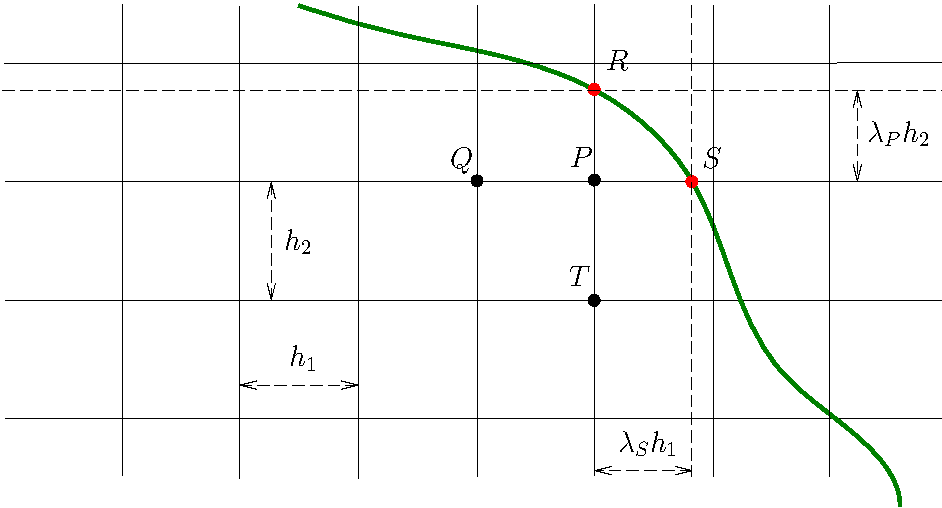
\includegraphics[width=11cm,height=8cm]{curved_bound_new.pdf}
\caption{}
\end{figure}

\vskip 0.3cm   Suppose that $P=(x,y)$ is an irregular grid
point, such that $S=(x+\lambda_{S}h_{1},y)$ and
$R=(x,y+\lambda_{R}h_{2})$ where $0<\lambda_{S,R}<1$ lie on the
boundary of ${\cal D}$ and the other two neighbouring grid points,
$Q=(x-h_{1},y)$ and $T=(x,y-h_{2})$, are inside ${\cal D}$ (see
Fig. 1). Then the derivatives of $u$ at point $P$ can be
approximated in the following manner. First, we expand
$u_{S}=u\vert_{S}$ and $u_{Q}=u\vert_{Q}$ in Taylor series at
point $P$:
\begin{eqnarray}
&&u_{S}=u_{P}+\lambda_{S}h_{1}\frac{\pr u}{\pr x}\biggm\vert_{P}+
\frac{(\lambda_{S}h_{1})^2}{2}\frac{\pr^2 u}{\pr x^2}\biggm\vert_{P}+O(h_{1}^3), \nonumber \\
&&u_{Q}=u_{P}-h_{1}\frac{\pr u}{\pr x}\biggm\vert_{P}+
\frac{h_{1}^2}{2}\frac{\pr^2 u}{\pr
x^2}\biggm\vert_{P}+O(h_{1}^3),  \nonumber
\end{eqnarray}
Multiplying the second equation by $\lambda_{S}^2$ and subtracting
the result from the first equation yields
\[
\frac{\pr u}{\pr
x}\biggm\vert_{P}=\frac{1}{h_{1}\lambda_{S}(1+\lambda_{S})} \left[
u_{S}-\lambda_{S}^2
u_{Q}-(1-\lambda_{S}^2)u_{P}\right]+O(h_{1}^2).
\]
Similarly, if we multiply the second equation by $\lambda_{S}$ and
add the result to the first equation yields, we can obtain the
formula for the second derivative with respect to $x$:
\[
\frac{\pr^2 u}{\pr
x^2}\biggm\vert_{P}=\frac{2}{h_{1}^2\lambda_{S}(1+\lambda_{S})}
\left[ u_{S}+\lambda_{S}
u_{Q}-(1+\lambda_{S})u_{P}\right]+O(h_{1}).
\]
Note that the truncation error of the formula for the second
derivative is $O(h_{1})$. To obtain a higher order accuracy, we
need to use one more grid point, e.g. point $(x-2h_1,y)$.

\vskip 0.3cm   Similarly, one can obtain the following
formulae for the derivatives with respect to $y$:
\begin{eqnarray}
&&\frac{\pr u}{\pr
y}\biggm\vert_{P}=\frac{1}{h_{2}\lambda_{R}(1+\lambda_{R})}
\left[ u_{R}-\lambda_{R}^2 u_{T}-(1-\lambda_{R}^2)u_{P}\right]+O(h_{2}^2), \nonumber \\
&&\frac{\pr^2 u}{\pr
y^2}\biggm\vert_{P}=\frac{2}{h_{2}^2\lambda_{R}(1+\lambda_{R})}
\left[ u_{R}+\lambda_{R}
u_{T}-(1+\lambda_{R})u_{P}\right]+O(h_{2}). \nonumber
\end{eqnarray}



%%%%%%%%%%%%%%%%%%%%%%%%%%%%%%%%%
%
% Lecture notes for Numerical Methods for Partial Differential Equations
%
% Chapter 4: Hyperbolic PDEs
%
%%%%%%%%%%%%%%%%%%%%%%%%%%%%%%%%%

% !TeX root = NumPDE_Lecture_notes.tex

\section{Hyperbolic partial differential equations}


\subsection{Wave equation}

 
We will illustrate the finite-difference
method for hyperbolic PDEs with the linear wave equation
\begin{equation}
\frac{\pr^{2} u}{\pr t^{2}}(x,t) - \alpha^{2}\frac{\pr^{2} u}{\pr
x^{2}}(x,t)=F(x,t), \quad a<x< b, \quad 0<t<T,   \label{1}
\end{equation}
subject to the boundary conditions
\begin{equation}
u(a, t) = u(b, t)=0 \quad \hbox{for} \quad t\in[0,T],   \label{2}
\end{equation}
and initial conditions
\begin{eqnarray}
&&u(x, 0) = f(x), \label{3} \\
&&\frac{\pr u}{\pr t}(x,0)=g(x)  \quad \hbox{for} \quad x\in[a,b],
\label{4}
\end{eqnarray}
where $f(x)$ and $g(x)$ are given functions.

   
First we choose integers $N$ and $M$ and
let $h=(b-a)/N$, $\tau=T/M$. Then we define the mesh points
$(x_{k}, t_{j})$:
\[
x_{k}=a+hk \quad(k=0,1,\dots,N), \quad t_{j}=\tau j
\quad(j=0,1,\dots,M).
\]


\subsubsection{Explicit method}
We approximate the second partial derivatives with respect to $t$
and $x$ at interior grid points using the central difference
formulas
\begin{eqnarray}
&&\frac{\pr^{2} u}{\pr t^{2}}(x_{k},t_{j})=
\frac{u(x_{k},t_{j+1})-2u(x_{k},t_{j})+u(x_{k},t_{j-1})}{\tau^{2}}-
\frac{\tau^{2}}{12}\frac{\pr^{4} u}{\pr t^{4}}(x_{k}, \mu_{j}), \nonumber \\
&&\frac{\pr^{2} u}{\pr x^{2}}(x_{k},t_{j})= \frac{u(x_{k+1},
t_{j})-2u(x_{k},t_{j})-u(x_{k-1}, t_{j})}{h^{2}}-
\frac{h^{2}}{12}\frac{\pr^{4} u}{\pr x^{4}}(\xi_{k}, t_{j}),
\nonumber
\end{eqnarray}
where $\mu_{j}\in(t_{j-1},t_{j+1})$ and
$\xi_{k}\in(x_{k-1},x_{k+1})$.

   
With these formulas, we approximate the
wave equation (\ref{1}) at the interior mesh points $(x_{k},
t_{j})$ for $k=1, 2, \dots, N-1$ and $j=1, 2, \dots$ by the
difference equation
\begin{equation}
\frac{w_{k,j+1}-2w_{kj}+w_{k,j-1}}{\tau^{2}}-\alpha^{2}
\frac{w_{k+1, j}-2w_{kj}+w_{k-1,j}}{h^{2}}=F_{kj}, \label{5}
\end{equation}
where $w_{kj}$ approximates $u(x_{k},t_{j})$ (i.e. $w_{kj}\approx
u(x_{k},t_{j})$).

    The local truncation error of the
difference equation (\ref{5}) is
\[
\tau_{ij}=\frac{\tau^{2}}{12}\frac{\pr^{4} u}{\pr t^{4}}(x_{k},
\mu_{j})-\alpha^2 \frac{h^{2}}{12}\frac{\pr^{4} u}{\pr
x^{4}}(\xi_{k}, t_{j})=O(\tau^{2}+h^{2}).
\]
Let
\[
\gamma\equiv\frac{\alpha\tau}{h}.
\]
Then equation (\ref{5}) can be written as
\begin{equation}
w_{k,j+1}=2\left(1-\gamma^{2}\right)w_{kj}+
\gamma^{2}\left(w_{k+1, j}+w_{k-1,j}\right)-w_{k,j-1}+\tau^2
F_{kj} , \label{6}
\end{equation}
for each $k=1, 2, \dots, N-1$ and $j=1, 2, \dots$. The boundary
conditions (\ref{2}) imply that
\begin{equation}
w_{0,j}=w_{N,j}=0 \quad \hbox{for each} \quad j=1, 2, \dots,
\label{7}
\end{equation}
and the initial condition (\ref{3}) yields
\begin{equation}
w_{k,0}=f(x_{k}) \quad \hbox{for each} \quad i=1, 2, \dots, N-1.
\label{8}
\end{equation}
Equation (\ref{5}) can be written in the matrix form
\begin{equation}
{\bf w}^{(j+1)}=A{\bf w}^{(j)}-{\bf w}^{(j-1)}+{\bf F}^{(j)},
\label{9}
\end{equation}
where
\begin{gather}
A=\left[
\begin{array}{cccccc}
2(1-\gamma^{2}) &\gamma^{2} &0      &\dots  &\dots &0 \\
\gamma^{2} &2(1-\gamma^{2}) &\gamma^{2} &\ddots  &     &\vdots \\
0      &\gamma^{2} &2(1-\gamma^{2}) &\gamma^{2} &\ddots &\vdots \\
\vdots &\ddots &\ddots &\ddots &\ddots &0 \\
\vdots &       &\ddots &\ddots &\ddots &\gamma^{2} \\
0      &\dots  &\dots  &0      &\gamma^{2} &2(1-\gamma^{2})
\end{array}\right], \\
{\bf w}^{(j)}=\left[
\begin{array}{c}
w_{1,j} \\
w_{2,j} \\
\vdots \\
\vdots \\
\vdots \\
w_{N-1,j}
\end{array}\right], \quad
{\bf F}^{(j)}=\left[
\begin{array}{c}
\tau^2 F_{1,j} \\
\tau^2 F_{2,j} \\
\vdots \\
\vdots \\
\vdots \\
\tau^2 F_{N-1,j}
\end{array}\right].
\label{77}
\end{gather}


\subsubsection{Initial conditions}
It is clear from Eq. (\ref{9}) that the $(j+1)$-st time step
requires the values from the $j$-th and $(j-1)$-st time steps. For
example, to compute $w_{k,2}$, we need values of $w_{k,0}$ and
$w_{k,1}$ for $k=1, 2, \dots, N-1$. The values of $w_{k,0}$ are
given by Eq. (\ref{8}), but values of $w_{k,1}$ must be obtained
from the other initial condition (\ref{4}).

The simplest way to approximate the initial
condition (\ref{4}) is to replace $\pr u/\pr t$ by the
forward-difference formula
\[
\frac{\pr u}{\pr
t}(x_{k},0)=\frac{u(x_{k},t_{1})-u(x_{k},0)}{\tau}-
\frac{\tau}{2}\frac{\pr^{2} u}{\pr t^{2}}(x_{k}, \mu), \quad 0<\mu
< \tau.
\]
It follows that
\[
u(x_{k},t_{1})=u(x_{k},0)+\tau \frac{\pr u}{\pr t}(x_{k},0)+
\frac{\tau^{2}}{2}\frac{\pr^{2} u}{\pr t^{2}}(x_{k}, \mu)=
f(x_{k})+\tau g(x_{k})+ \frac{\tau^{2}}{2}\frac{\pr^{2} u}{\pr
t^{2}}(x_{k}, \mu).
\]
Hence,
\begin{equation}
w_{k,1}=f(x_{k})+\tau g(x_{k}). \label{10}
\end{equation}
However, this equation has local truncation error of order
$O(\tau)$. A better approximation to $u(x_{k},t_{1})$ can be
obtained as follows. Expanding $u(x_{k},t_{1})$ in Taylor's series
in $t$ at $(x_{k},0)$, we obtain
\begin{equation}
\frac{u(x_{k},t_{1})-u(x_{k},0)}{\tau}=\frac{\pr u}{\pr
t}(x_{k},0)+ \frac{\tau}{2}\frac{\pr^{2} u}{\pr t^{2}}(x_{k},0)+
\frac{\tau^{2}}{6}\frac{\pr^{3} u}{\pr t^{3}}(x_{k}, \mu)
\label{11}
\end{equation}
for some $\mu\in(0,t_{1})$. Suppose that the wave equation also
holds on the initial line, i.e.
\[
\frac{\pr^{2} u}{\pr t^{2}}(x_{k},0) - \alpha^{2}\frac{\pr^{2}
u}{\pr x^{2}}(x_{k},0)=0 \quad \hbox{for} \quad k=0,1, \dots, N.
\]
Then
\[
\frac{\pr^{2} u}{\pr t^{2}}(x_{k},0) = \alpha^{2}\frac{\pr^{2}
u}{\pr x^{2}}(x_{k},0)+F((x_{k},0)=
\alpha^{2}f^{\prime\prime}(x_{k})+F(x_{k},0).
\]
This equation and Eq. (\ref{11}) yield
\[
u(x_{k},t_{1})=f(x_{k})+\tau g(x_{k})+
\frac{\tau^{2}}{2}\left[\alpha^{2}f^{\prime\prime}(x_{k})+F(x_{k},0)\right]+
\frac{\tau^{3}}{6}\frac{\pr^{3} u}{\pr t^{3}}(x_{k}, \mu).
\]
Hence,
\begin{equation}
w_{k,1}=f(x_{k})+\tau g(x_{k})+
\frac{\tau^{2}}{2}\left[\alpha^{2}f^{\prime\prime}(x_{k})+F(x_{k},0)\right].
\label{12}
\end{equation}
This is an approximation with local truncation error $O(\tau^{2})$
for each $k=1, 2, \dots, N-1$. If $f^{\prime\prime}(x_{k})$ is not
readily available, we can use the central difference formula to
approximate it.


\subsubsection{Stability}
The finite-difference method described
above is explicit and has local truncation error
$O(\tau^{2}+h^{2})$. Now we will investigate the stability of the
method. To do this, we employ the Fourier method. Since the
difference equation (\ref{5}) is linear, the perturbation $z_{kj}$
satisfies the equation
\[
\frac{z_{k,j+1}-2z_{kj}+z_{k,j-1}}{\tau^{2}}-\alpha^{2}
\frac{z_{k+1, j}-2z_{kj}-z_{k-1,j}}{h^{2}}=0, 
\]
for $k=1,2, \dots,N-1, j=1,2, \dots$,
which is a homogeneous version of Eq. (\ref{5}). Substituting
$z_{k,j}=\rho_{q}^{j}e^{iqx_{k}}$ into this equation, we obtain
\[
e^{iqx_{k}}\left(\rho_{q}^{j+1}-2\rho_{q}^{j}+\rho_{q}^{j-1}\right)-
\gamma^{2}\rho_{q}^{j}
\left(e^{iqx_{k+1}}-2e^{iqx_{k}}+e^{iqx_{k-1}}\right)=0
\]
or
\begin{multline*}
\rho_{q}^{2}-2\rho_{q}\left[1+
\frac{\gamma^{2}}{2}\left(e^{iqh}-2+e^{-iqh}\right)\right]+1=0\\
\Rightarrow \quad \rho_{q}^{2}-2\rho_{q}\left[1-
2\gamma^{2}\sin^{2} \frac{qh}{2}\right]+1=0.
\end{multline*}
Thus, $\rho_{q}$ is a root of the quadratic equation
\[
\rho_{q}^{2}-2a\rho_{q}+1=0, \quad a\equiv 1- 2\gamma^{2}\sin^{2}
\frac{qh}{2}.
\]
Its roots are $\rho^{\pm}_{q}=a\pm\sqrt{a^{2}-1}$, so that the
product of the roots is equal to 1 ($\rho_{q}^{+}\rho_{q}^{-}=1$).
It follows that the stability condition $\vert\rho_{q}\vert \leq
1$ can be satisfied only if $\vert\rho_{q}^{+}\vert
=\vert\rho_{q}^{-}\vert = 1$. This means that the roots must be
complex conjugate. Hence, we must have
\[
a^{2}-1\leq 0 \quad \hbox{or} \quad \left\vert 1-
2\gamma^{2}\sin^{2}\frac{qh}{2}\right\vert \leq 1  \quad
\Rightarrow \quad -1\leq 1- 2\gamma^{2}\sin^{2}\frac{qh}{2}.
\]
The last inequality is satisfied for all $q$ if $\gamma\leq 1$. It
can be shown that if $\gamma=1$, then for certain modes $q$ (e.g.
for $q$ such that $qh=\pi$), the above quadratic equation has a
double root $\rho_{q}$, which results in a week instability: in
the limit $\tau\to 0$, their amplitudes grow linearly in $j$.
Therefore, the stability condition is
\[
\gamma <1 \quad \hbox{or} \quad \alpha\tau < h.
\]
Thus, the above explicit finite-difference method is conditionally
stable.


\subsubsection{Implicit method}
To obtain an {\it unconditionally} stable
method, we consider the difference equation in which the second
derivative with respect to $x$ is approximated by the central
difference formula averaged over the three time steps: $j+1$, $j$
and $j-1$.

    Let
\[
\delta_{x}^2 w_{kj}=w_{k+1,j}-2w_{k,j}+w_{k-1,j}.
\]
Consider the difference equation
\begin{equation}
w_{k,j+1}-2w_{kj}+w_{k,j-1}-\gamma^{2} \left[\sigma \delta_{x}^2
w_{k,j+1}+(1-2\sigma)\delta_{x}^2 w_{k,j} +\sigma \delta_{x}^2
w_{k,j-1}\right]=\tau^2 F_{kj}, \label{15}
\end{equation}
where $\sigma$ is an arbitrary parameter. 
An alternative way of writing this is in terms of the second order central
difference operator $\delta_t^2$,
\begin{equation}
w_{k,j+1}-2w_{kj}+w_{k,j-1}-\gamma^{2} \delta_{x}^2 w_{k,j} 
-\sigma\gamma^2 \delta_t^2\delta_{x}^2w_{k,j}=\tau^2 F_{kj}.
\end{equation}
For $\sigma=0$ we have the 
explicit method discussed in the previous section. 
For $\sigma\neq 0$ there is an additional term
\begin{equation}
-\sigma \gamma^2\delta_t^2\delta_{x}^2w_{k,j}
=-\sigma\tau^4\frac{\partial^4}{\partial_t^2\partial_x^2}u_{k,j}
+O(\tau^6+\tau^4h^2).\label{est}
\end{equation}
This only gives an $O(\tau^2)$ contribution to the truncation error
and thus the truncation error of this method is still $O(\tau^2+h^2)$
for any value of $\sigma$.

For positive $\sigma$ this extra term \eqref{est} will have a stabilising
effect.
We investigate the stability of the
method by the Fourier method. The perturbation
$z_{kj}$ satisfies the equation
\[
z_{k,j+1}-2z_{kj}+z_{k,j-1}-\gamma^{2} \left[\sigma \delta_{x}^2
z_{k,j+1}+(1-2\sigma)\delta_{x}^2 z_{k,j} +\sigma \delta_{x}^2
z_{k,j-1}\right]=0, 
\]
for  $k=1,2, \dots, N-1, j=1,2, \dots$.
This is the homogeneous version of Eq. (\ref{15}). Substituting
$z_{k,j}=\rho_{q}^{j}e^{iqx_{k}}$ into this equation, we obtain
\begin{multline*}
e^{iqx_{k}}\left(\rho_{q}^{j+1}-2\rho_{q}^{j}+\rho_{q}^{j-1}\right)\\-
\gamma^{2}\left[\sigma\rho_{q}^{j+1}+(1-2\sigma)\rho_{q}^{j}+\sigma\rho_{q}^{j-1}\right]
\left(e^{iqx_{k+1}}-2e^{iqx_{k}}+e^{iqx_{k-1}}\right)=0
\end{multline*}
or
\[
\left(\rho_{q}^{2}-2\rho_{q}+1\right)+
4\gamma^{2}\sin^{2}\frac{qh}{2}\left[\sigma\rho_{q}^{2}+(1-2\sigma)\rho_{q}+\sigma\right]=0.
\]
Hence, $\rho_{q}$ satisfies the quadratic equation
\begin{equation}
\rho_{q}^{2}-2a\rho_{q}+1=0, \label{16}
\end{equation}
where
\[
a\equiv
\frac{1-2\gamma^{2}(1-2\sigma)\sin^{2}\frac{qh}{2}}{1+4\gamma^{2}\sigma\sin^{2}\frac{qh}{2}}.
\]
Again, the method can be stable only if Eq. (\ref{16}) has complex
conjugate roots. This implies that
\begin{multline*}
a^{2}-1<0 \quad \Rightarrow \quad \left\vert
\frac{1-2\gamma^{2}(1-2\sigma)\sin^{2}\frac{qh}{2}}{1+4\gamma^{2}\sigma\sin^{2}\frac{qh}{2}}
\right\vert \leq 1 \\ 
\Rightarrow \quad -1\leq
\frac{1-2\gamma^{2}(1-2\sigma)\sin^{2}\frac{qh}{2}}{1+4\gamma^{2}\sigma\sin^{2}\frac{qh}{2}}.
\end{multline*}
The last inequality is equivalent to
\[
2-2\gamma^{2}(1-2\sigma)\sin^{2}\frac{qh}{2}+4\gamma^{2}\sigma\sin^{2}\frac{qh}{2}\geq
0
\]
or
\[
1-\gamma^{2}(1-4\sigma)\sin^{2}\frac{qh}{2}\geq 0.
\]
Evidently, if $\sigma \geq 1/4$, this inequality is satisfied for
all $q$, irrespective of the value of $\gamma$. Thus, if
$\sigma\in[1/4,1/2]$, then the above implicit method is
unconditionally stable.



\subsection{Hyperbolic systems of first-order
partial differential equations}

\vskip 0.3cm
 
Since the equations of physics (e.g., fluid mechanics) are
based upon conservation laws, it convenient to use a form of the equations,
called the {\it divergence form} (or {\it flux-conservative} form, or
{\it conservation-law} form).
A system of equations
\begin{equation}
{\bf U}_{t} + \left[{\bf F}({\bf U})\right]_{x} =0, \label{p1}
\end{equation}
where ${\bf U}(x,t)$ is a vector function with $n$ components and ${\bf F}$ is a
(in general, nonlinear) vector function (with $n$ components) of the vector
${\bf U}$, is called a system of conservation laws.

\vskip 0.3cm
 
The wave equation
\begin{equation}
\frac{\pr^{2} u}{\pr t^{2}}(x,t) - \alpha^{2}\frac{\pr^{2} u}{\pr x^{2}}(x,t)=0  \label{p2}
\end{equation}
can be easily written in the conservative form (\ref{p1}). Indeed, if
\[
r=\alpha u_{x} \quad {\rm and} \quad s=u_{t},
\]
then Eq. (\ref{p2}) is equivalent to the system:
\begin{equation}
\frac{\pr}{\pr t}
\left(
\begin{array}{c}
r \\
s
\end{array}
\right) +
\frac{\pr}{\pr x}
\left(
\begin{array}{c}
-\alpha s \\
-\alpha r
\end{array}
\right)=0, \label{p3}
\end{equation}
which has the form of Eq. (\ref{p1}).

\vskip 0.3cm
 
In what follows we will discuss only the pure initial value problem
(putting aside problems with boundary conditions).

 
 
{\bf Methods with error $O(\tau +h^2)$.} First we consider the simplest case of Eq. (\ref{p1}) when ${\bf U}$ has only
one component. Namely, we start with the scalar equation
\begin{equation}
u_{t} + \alpha u_{x} =0, \label{p4}
\end{equation}
where $\alpha$ is a constant. Use the forward-difference formula
for $u_{t}$ and the central difference formula for $u_{x}$, we obtain
the following finite-difference approximation of Eq. (\ref{p4}):
\begin{equation}
\frac{w_{k,j+1}-w_{k,j}}{\tau} + \alpha \frac{w_{k+1,j}-w_{k-1,j}}{2h} =0, \label{p5}
\end{equation}
where $w_{k,j}$ denotes the discrete approximation to $u(x_{k},t_{j})$, $\tau$ and $h$
are the step sizes in $t$ and $x$, respectively. Equation (\ref{p5})
represent an explicit method whose local truncation error is $O(\tau+h^2)$.

 
 
To find out whether this method is stable, we use the Fourier method. The error
(perturbation) $z_{k,j}$ satisfies the same equation as Eq. (\ref{p5}). And we look
for a solution in the form $z_{k,j}=\rho^{j}_{q}e^{iqx_{k}}$ where $q\in{\mathbb R}$.
Substitution of $z_{k,j}$ in Eq. (\ref{p5}) yields
\[
\rho_{q}-1+\frac{\gamma}{2}\left(e^{iqh}-e^{-iqh}\right)=0
\]
or
\[
\rho_{q}=1-i\gamma\sin(qh),
\]
where $\gamma=\alpha\tau/h$. Evidently,
\[
\vert\rho_{q}\vert^2=1+\gamma^2\sin^2(qh) >1 .
\]
for all $q$ for which $\sin(qh)\neq 0$. Therefore,
the method is unconditionally unstable.



   
It turns out that a stable method can be obtained simply by replacing $u_{k,j}$ in the forward-difference formula for
the time derivative
\[
u_{t}\approx \frac{u_{k,j+1}-u_{k,j}}{\tau}
\]
by its average
\[
\frac{1}{2}\left(u_{k+1,j}+u_{k-1,j}\right).
\]
This transforms Eq. (\ref{p5}) to
\[
\frac{1}{\tau}\left(w_{k,j+1}-\frac{1}{2}[w_{k+1,j}+w_{k-1,j}]\right) + \alpha \frac{w_{k+1,j}-w_{k-1,j}}{2h} =0,
\]
or, equivalently,
\begin{equation}
w_{k,j+1}=\frac{1}{2}[w_{k+1,j}+w_{k-1,j}] - \frac{\gamma}{2}\left[w_{k+1,j}-w_{k-1,j}\right] . \label{p6}
\end{equation}
Equation (\ref{p6}) is called the {\it Lax} scheme.
Let us now investigate its stability. Substitution of $z_{k,j}=\rho^{j}_{q}e^{iqx_{k}}$ leads to
\[
\rho_{q}=\frac{1}{2}\left(e^{iqh}+e^{-iqh}\right)
-\frac{\gamma}{2}\left(e^{iqh}-e^{-iqh}\right) \quad \Rightarrow \quad
\rho_{q}=\cos(qh)-i\gamma\sin(qh).
\]
If follows that
\[
\vert\rho_{q}\vert^2=\cos^2(qh)+\gamma^2\sin^2(qh) \quad \Leftrightarrow \quad
\vert\rho_{q}\vert^2=1+(\gamma^2-1)\sin^2(qh).
\]
The stability condition $\vert \rho_{q}\vert\leq 1$ leads to the requirement
\begin{equation}
\gamma \leq 1 \quad {\rm or} \quad \tau \leq \frac{h}{\alpha}. \label{p7}
\end{equation}
This inequality is called the {\it Courant} stability criterion. The surprising result that the above simple modification
can stabilize an unconditionally stable method can be explained as follows. First, we can rewrite
Eq. (\ref{p6}) as
\begin{equation}
\frac{w_{k,j+1}-w_{k,j}}{\tau}+
 \alpha\frac{w_{k+1,j}-w_{k-1,j}}{2h}= \frac{h^2}{2\tau}\frac{w_{k+1,j}-2w_{k,j}+w_{k-1,j}}{h^2}. \label{p8}
\end{equation}
If the term on the right side of this equation was zero, we would have the unconditionally unstable
method (\ref{p5}). For small $\tau$ and $h$ the difference equation (\ref{p8}) approximates
the equation
\begin{equation}
u_{t}+\alpha u_{x}=\frac{h^2}{2\tau}u_{xx}. \label{p9}
\end{equation}
Thus, effectively we have added a diffusion (or dissipation) term
to the equation, and this made the new method stable. The Lax scheme is said to have
{\it numerical dissipation} or {\it numerical viscosity}.

 
 
When we have a system of equations rather than a scalar equation, the stability analysis becomes
slightly more complicated. As an example, consider the wave equation written in the form  (\ref{p3}).
The Lax scheme for Eq. (\ref{p3}) is
\begin{eqnarray}
&&r_{k,j+1}=\frac{1}{2}[r_{k+1,j}+r_{k-1,j}] + \frac{\gamma}{2}\left[s_{k+1,j}-s_{k-1,j}\right], \nonumber \\
&&s_{k,j+1}=\frac{1}{2}[s_{k+1,j}+s_{k-1,j}] +
\frac{\gamma}{2}\left[r_{k+1,j}-r_{k-1,j}\right], \label{p10}
\end{eqnarray}
where $r_{kj}$ and $s_{kj}$ denote approximations to $r(x_{k},t_{j})$ and $s(x_{k},t_{j})$, respectively.
To investigate the stability of (\ref{p10}), we assume that
\begin{equation}
\left(
\begin{array}{c}
r_{kj} \\
s_{kj}
\end{array}
\right)=\rho_{q}^{j}e^{iqx_{k}}
\left(
\begin{array}{c}
r^{(0)} \\
s^{(0)}
\end{array}
\right), \label{p11}
\end{equation}
where $r^{(0)}$ and $s^{(0)}$ are constants.
Substituting this in Eq. (\ref{p10}), we obtain
\begin{equation}
\left(
\begin{array}{cc}
\cos(qh)-\rho_{q} &i\gamma\sin(qh) \\
i\gamma\sin(qh)   &\cos(qh)-\rho_{q}
\end{array}
\right)
\left(
\begin{array}{c}
r^{(0)} \\
s^{(0)}
\end{array}
\right)=0. \nonumber
\end{equation}
This system has a nonzero solution only if the determinant of the matrix on the left side
is zero. This gives us
\[
(\cos(qh)-\rho_{q})^2+\gamma^2\sin^2(qh)=0 \quad \Rightarrow \quad
\rho_{q}=\cos(qh)\pm i\gamma\sin(qh).
\]
The stability condition is that both roots satisfy the inequality $\vert\rho_{q}\vert\leq 1$, which again
leads us to the Courant condition (\ref{p7}).


 
 
For the system of conservation laws (\ref{p1}), the Lax
method is given by
\begin{equation}
{\bf U}_{k,j+1}=\frac{1}{2}\left({\bf U}_{k+1,j}+{\bf U}_{k-1,j}\right) -\frac{\tau}{2h}
\left[{\bf F}({\bf U}_{k+1,j})-{\bf F}({\bf U}_{k-1,j})\right]. \label{ppp1}
\end{equation}
Here ${\bf U}_{k,j}\approx {\bf U}(x_{k},t_{j})$.



 
 
\textbf{Methods with error $O(\tau^2 +h^2$).} All the schemes
discussed above have local truncation error $O(\tau+h^2)$. It is
desirable to have a method whose truncation error is quadratic both
in space and time. We will discuss two such methods. First of them
is called the `leapfrog' method in which we use the
central-difference formula for derivatives in both $x$ and $t$. For
Eq. (\ref{p4}), this method is given by
\begin{equation}
\frac{w_{k,j+1}-w_{k,j-1}}{2\tau} + \alpha\frac{w_{k+1,j}-w_{k-1,j}}{2h}=0 . \label{p12}
\end{equation}
The standard stability analysis yields the following equation for $\rho_{q}$:
\[
\rho^2_{q}+2i\gamma\sin(qh)\rho_{q}-1=0.
\]
It follows that
\[
\rho_{q}=-i\gamma\sin(qh)\pm\sqrt{1-\gamma^2\sin^2(qh)}.
\]
If the Courant condition (\ref{p7}) is satisfied, i.e. $\gamma\leq 1$, then
$\vert \rho_{q}\vert=1$, and the method is stable. If $\gamma > 1$, then
for $q$ such that $\sin(qh)=1$, we have
\[
\rho_{q}=-i\gamma\pm i \sqrt{\gamma^2-1}.
\]
For the second root (with `minus' sign), we obtain
\[
\vert\rho_{q}\vert=\gamma+\sqrt{\gamma^2-1} > 1.
\]
Therefore, the Courant condition is the necessary and sufficient condition for stability of the
`leapfrog' method.


 
 
For the system of conservation laws (\ref{p1}), the `leapfrog' method is given by
\begin{equation}
\frac{{\bf U}_{k,j+1}-{\bf U}_{k,j-1}}{2\tau} +
\frac{{\bf F}({\bf U}_{k+1,j})-{\bf F}({\bf U}_{k-1,j})}{2h} =0. \label{p13}
\end{equation}
Here ${\bf U}_{k,j}\approx {\bf U}(x_{k},t_{j})$.
Note that in order to use Eq. (\ref{p12}) or Eq. (\ref{p13}), one needs to know
$w_{k,0}$ and $w_{k,1}$ (or ${\bf U}_{k,0}$ and ${\bf U}_{k,1}$).

 
 
The other method is called the two-step Lax-Wendroff scheme. First, we compute
intermediate values $w_{k+\frac{1}{2},j+\frac{1}{2}}$ at the half timesteps
$t_{j+\frac{1}{2}}$ and the half mesh point $x_{k+\frac{1}{2}}$ using the Lax method:
\begin{equation}
w_{k+\frac{1}{2},j+\frac{1}{2}}=\frac{1}{2}\left[w_{k+1,j}+w_{k,j}\right] -
\frac{\gamma}{2}\left[w_{k+1,j}-w_{k,j}\right]. \label{p14}
\end{equation}
Then, we compute the updated values using the equation:
\begin{equation}
w_{k,j+1}=w_{k,j}-
\gamma\left[w_{k+\frac{1}{2},j+\frac{1}{2}}-w_{k-\frac{1}{2},j+\frac{1}{2}}\right]. \label{p15}
\end{equation}
Substituting (\ref{p14}) in (\ref{p15}), we can rewrite the method in the form:
\[\begin{split}
w_{k,j+1}=w_{k,j}-
\gamma&\left[
\frac{1}{2}  \left(w_{k+1,j}+w_{k,j}\right)-
\frac{\gamma}{2}\left(w_{k+1,j}-w_{k,j}\right)
\right.\\
&\left.-\frac{1}{2}\left(w_{k,j}+w_{k-1,j}\right)+
\frac{\gamma}{2}\left(w_{k,j}-w_{k-1,j}\right)\right].
\end{split}\]
or, equivalently,
\begin{equation}
w_{k,j+1}=w_{k,j}-
\gamma\left[\frac{1}{2}\left(w_{k+1,j}-w_{k-1,j}\right)-
\frac{\gamma}{2}\left(w_{k+1,j}-2w_{k,j}+w_{k-1,j}\right)\right]. \label{p16}
\end{equation}
One can show that the local truncation error of Eq. (\ref{p16}) is $O(\tau^2+h^2)$ (prove it!). The stability
analysis leads to
\[
\rho_{q}=1-i\gamma\sin(qh)-\gamma^2[1-\cos(qh)].
\]
It follows that
\[
\vert\rho_{q}\vert^2=1-\gamma^2(1-\gamma^2)[1-\cos(qh)]^2.
\]
Again, the stability condition is satisfied provided that $\gamma\leq 1$, i.e.
if the Courant condition (\ref{p7}) holds.

 
 
For the system of conservation laws (\ref{p1}), the Lax-Wendroff scheme has the form
\begin{eqnarray}
&&{\bf U}_{k+\frac{1}{2},j+\frac{1}{2}}=\frac{1}{2}\left[{\bf U}_{k+1,j}+{\bf U}_{k,j}\right] -
\frac{\tau}{2h}\left[{\bf F}({\bf U}_{k+1,j})-{\bf F}({\bf U}_{k,j})\right], \nonumber \\
&&{\bf U}_{k,j+1}={\bf U}_{k,j}-
\frac{\tau}{h}\left[{\bf F}({\bf U}_{k+\frac{1}{2},j+\frac{1}{2}})-
{\bf F}({\bf U}_{k-\frac{1}{2},j+\frac{1}{2}})\right]. \label{p17}
\end{eqnarray}






%%%%%%%%%%%%%%%%%%%%%%%%%%%%%%%%%%%%%%%%%%%%%%%%%%%%%%%%%%%%%%%%%%%%%%%%%%%%%%%%%%%%%%%%%%%%%%%%%%%%%%%%%%%%%%%%%


\setcounter{equation}{0}
\renewcommand{\theequation}{A.\arabic{equation}}

\section{Appendix A}

 
We want to show that if $u\in C^{4}(D)$ (where $D=\{(x,y)\, \vert \ 0<x<1, \ 0<y<1 \, \}$)
is the exact solution of the boundary-value
problem (\ref{gg1}), (\ref{gg2}) and $w_{ij}$ ($i,j=1,2, \dots,N-1$) satisfy Eq. (\ref{gg5}), then
\[
\left\vert w_{ij}-u(x_{i}, y_{j})\right\vert \leq Ah^{2},
\]
where $A$ is independent of $h$.

\vskip 0.3cm
 
{\bf Solution.} To solve this problem, we need first to prove 2 auxiliary propositions.

\vskip 0.3cm
 
{\bf Proposition 1.} {\it Let $v_{ij}$ for $i,j=0,1\dots, N$ be a set of real numbers satisfying
the inequality}
\begin{equation}
v_{i+1,j}+v_{i-1,j}+v_{i,j+1}+v_{i,j-1}-4v_{i,j}\geq 0, \label{21}
\end{equation}
for all
$i,j=1,2,\dots,N-1$ {\it (i.e at all internal mesh points). Then
the maximum of $v_{ij}$ is attained at least at one of the boundary points.}

 
 
{\bf Proof.} Assume that the above statement is not true, i.e. that the maximum is attained at
an internal point (there may be several such points). Let $(m,n)$ be a point at which the maximum is attained and
which corresponds to the maximum value of $m$, i.e.
\[
v_{m,n}=\max_{0\leq i,j\leq N}v_{ij} \quad \hbox{and} \quad
v_{m,n}>v_{m+1,n}.
\]
Then,
\begin{equation}
v_{m+1,n}-v_{m,n}+(v_{m-1,n}-v_{m,n})+(v_{m,n+1}-v_{m,n})
+(v_{m,n-1}-v_{m,n})\leq v_{m+1,n}-v_{m,n}<0. \label{22}
\end{equation}
Evidently, (\ref{22}) is in contradiction with (\ref{21}). Thus, our assumption is wrong, which proves
the proposition.

 
 
{\bf Proposition 2.} {\it Let $v_{ij}$ for $i,j=0,1\dots, N$ be a set of real numbers satisfying
the inequality}
\begin{equation}
v_{i+1,j}+v_{i-1,j}+v_{i,j+1}+v_{i,j-1}-4v_{i,j}\leq 0, \label{23}
\end{equation}
for all
$i,j=1,2,\dots,N-1$ {\it (i.e at all internal mesh points). Then
the minimum of $v_{ij}$ is attained at least at one of the boundary points.}

    {\bf Proof.} Assume that the above
statement is not true, i.e. that the minimum is attained at an
internal point (there may be several such points). Let $(m,n)$ be
a point at which the minimum is attained and which corresponds to
the minimum value of $m$, i.e.
\[
v_{m,n}=\min_{0\leq i,j\leq N}v_{ij} \quad \hbox{and} \quad
v_{m,n}<v_{m-1,n}.
\]
Then we have
\begin{equation}
v_{m+1,n}-v_{m,n}+(v_{m-1,n}-v_{m,n})+(v_{m,n+1}-v_{m,n})
+(v_{m,n-1}-v_{m,n})\geq v_{m-1,n}-v_{m,n}>0. \label{24}
\end{equation}
Evidently, (\ref{24}) contradicts inequality (\ref{23}). So, our assumption is wrong, which proves
the proposition.

 
 
Now we are ready to prove the original statement. If $z_{ij}=w_{ij}-u_{ij}$, then, it follows from Eq. (\ref{g5}) that
\[
z_{i+1,j}+z_{i-1,j}+z_{i,j+1}+z_{i,j-1}-4z_{i,j}=h^{2}f(x_{j},y_{j})
-u_{i+1,j}-u_{i-1,j}-u_{i,j+1}-u_{i,j-1}+4u_{i,j},
\]
where $u_{ij}\equiv u(x_{i}, y_{j})$. Comparing the right hand side of this equation
with the definition of local truncation error $\tau_{ij}(h)$, we find that
\begin{equation}
z_{i+1,j}+z_{i-1,j}+z_{i,j+1}+z_{i,j-1}-4z_{i,j}=-h^{2}\tau_{ij}(h). \label{29}
\end{equation}
Let $R={\rm diam}\, {\cal D}/2=\sqrt{2}/2$. We define the auxiliary function $Q(x, y)$ by the formula
\[
Q(x, y)=\frac{1}{4}\left[R^{2}-\left(x-\frac{1}{2}\right)^{2}
-\left(y-\frac{1}{2}\right)^{2}\right]E,
\]
where
\[
E\equiv \max_{1\leq i,j\leq N-1}\vert\tau_{ij}(h)\vert
\]
is the maximum truncation error. $Q$ is a quadratic polynomial in $x$ and $y$, and therefore
\begin{equation}
Q_{i+1,j}+Q_{i-1,j}+Q_{i,j+1}+Q_{i,j-1}-4Q_{i,j}=
h^{2}\left(\frac{\pr^{2}Q}{\pr x^{2}}+\frac{\pr^{2}Q}{\pr x^{2}}\right)\Biggm\vert_{x=x_{i}, y=y_{j}}=
-h^{2}E, \label{30}
\end{equation}
where $Q_{ij}\equiv Q(x_{i}, y_{j})$.

 
 
Let $v_{ij}=z_{ij}-Q_{ij}$. Then, according to (\ref{29}) and (\ref{30})
\[
v_{i+1,j}+v_{i-1,j}+v_{i,j+1}+v_{i,j-1}-4v_{i,j}=h^{2}(E-\tau_{ij})\geq 0. \label{31}
\]
By Proposition 1, maximum of $v_{ij}$ is attained on the boundary. But on the boundary, we have
\[
v_{ij}=z_{ij}-Q_{ij}=-Q_{ij}\leq 0.
\]
Thus,
\[
z_{ij}\leq Q_{ij} \quad \hbox{for} \quad i,j=0,1,\dots, N.
\]


 
 
Similarly, if $v_{ij}=z_{ij}+Q_{ij}$, then, according to (\ref{29}) and (\ref{30})
\[
v_{i+1,j}+v_{i-1,j}+v_{i,j+1}+v_{i,j-1}-4v_{i,j}=h^{2}(-E-\tau_{ij})\leq 0.
\]
By Proposition 2, minimum of $v_{ij}$ is attained on the boundary. But on the boundary, we have
\[
v_{ij}=z_{ij}+Q_{ij}=Q_{ij}\geq 0.
\]
Hence,
\[
-Q_{ij}\leq z_{ij} \quad \hbox{for} \quad i,j=0,1,\dots, N.
\]
Thus,
\[
-Q_{ij}\leq z_{ij}\leq Q_{ij} \quad \Rightarrow \quad \vert z_{ij}\vert \leq \vert Q_{ij}\vert
\quad \Rightarrow \quad \max_{0\leq i,j\leq N}\vert z_{ij}\vert \leq
\max_{0\leq i,j\leq N}\vert Q_{ij}\vert=\frac{R^{2}}{4}E
\]
It can be shown that
\[
\tau_{ij}(h)=\frac{h^{2}}{24}\left[\frac{\pr^{4} u}{\pr x^{4}}(\xi^{+}_{i},y_{j})+
\frac{\pr^{4} u}{\pr x^{4}}(\xi^{-}_{i},y_{j})
+\frac{\pr^{4} u}{\pr y^{4}}(x_{i},\mu^{+}_{j})+
\frac{\pr^{4} u}{\pr y^{4}}(x_{i},\mu^{-}_{j})\right].
\]
Let $M=\max\{M_{1}, M_{2}\}$ where
\[
M_{1}=\max_{(x,y)\in{\cal D}} \left\vert \frac{\pr^{4}u}{\pr x^{4}}\right\vert, \quad
M_{2}=\max_{(x,y)\in{\cal D}} \left\vert \frac{\pr^{4}u}{\pr y^{4}}\right\vert.
\]
Then
\[
E=\max_{0\leq i,j\leq N}\vert \tau_{ij}(h)\vert\leq \frac{Mh^{2}}{6}.
\]
Finally, we obtain
\[
\max_{0\leq i,j\leq N}\vert z_{ij}\vert \leq \frac{R^{2}M}{24}h^{2}.
\]








\end{document}
